\documentclass[11pt]{extarticle}
\usepackage{fullpage,subfigure,fancyhdr}
\usepackage{color}
\usepackage{textcomp}
\usepackage{verbatim}
\usepackage{times}
\usepackage{amsfonts,amsmath,amssymb,amsthm}
\usepackage{textcomp}
\usepackage{url}
\usepackage{mdwlist}
\usepackage{wrapfig,caption,subfigure,sidecap}
\usepackage{xspace}
\usepackage{algorithm}
\usepackage{algpseudocode}
\usepackage{graphicx}
\usepackage[colorlinks=true,pagebackref,linkcolor=magenta]{hyperref}
\usepackage[sort&compress,comma,square,numbers]{natbib}
\usepackage{pict2e}
\usepackage[nottoc,numbib]{tocbibind}
\usepackage{paralist}
\usepackage{multicol}
\usepackage{lettrine}
\usepackage{helvet}
\usepackage{authblk}
\usepackage[linecolor=dark_blue, linewidth=1.5pt, skipabove=4pt, nobreak=true]{mdframed}
\usepackage{tikz}
\usepackage{graphicx}
\usepackage{neurodata}
% \usepackage{trackchanges}
% \usepackage{mcode}

\renewcommand{\familydefault}{\sfdefault}
\definecolor{MyGray}{rgb}{0.7,0.7,0.7}

% \numberwithin{figure}{section}
% \numberwithin{table}{section}
% \numberwithin{algorithm}{section}

% \pagestyle{fancy}
% \oddsidemargin=-0.5in 
% \evensidemargin=-0.5in
\textwidth=6.5in 
\headwidth=6.5in
\textheight=9.0in 
\headheight=0.0pt
\topmargin=0.0in
\headsep=0.0in
\renewcommand{\headrulewidth}{0pt}

\setlength{\parindent}{0em}
\setlength{\parskip}{0.5em}

%%%%% COLOR STUFF %%%%%%%%%%
\newcommand{\db}[1]{{\color{dark_blue}{#1}}}
\newcommand{\bb}[1]{{\textbf{\db{#1}}}}
\newcommand{\cb}[1]{\centering{{\textbf{\db{#1}}}}}

\definecolor{MyPlum}{rgb}{0.3,0,0.3}
\definecolor{MyOrange}{rgb}{1,0.5,0}
\definecolor{deep_blue}{rgb}{0,.2,.5}
\definecolor{dark_blue}{rgb}{0,.15,.5}

\newcommand{\marta}[1]{{\color{red}{\it marta: #1}}}
\newcommand{\youngser}[1]{{\color{green}{\it youngser: #1}}}
\newcommand{\brett}[1]{{\color{blue}{\it brett says: #1}}}
\newcommand{\jovo}[1]{{\color{magenta}{\it JoVo: #1}}}
\newcommand{\rb}[1]{{\color{red}{\it rb: #1}}}
\newcommand{\bro}[1]{{\color{blue}{\it youngser: #1}}}
\newcommand{\agastya}[1]{{\color{red}{\it agastya: #1}}}
\providecommand{\tg}[1]{\textcolor{green}{#1}}
\providecommand{\tb}[1]{\textcolor{blue}{#1}}
\providecommand{\tr}[1]{\textcolor{red}{#1}}
\providecommand{\tk}[1]{\textcolor{black}{#1}}
\providecommand{\twhite}[1]{\textcolor{white}{#1}}

\newcommand{\Linefor}[2]{%
    \State \algorithmicfor\ {#1}\ \algorithmicdo\ {#2} \algorithmicend\ \algorithmicfor%
}
\newcommand{\Lineif}[2]{%
    \State \algorithmicif\ {#1}\ \algorithmicdo\ {#2} \algorithmicend\ \algorithmicif%
}


%%%%%%%%% MATH OPERATORS %%%%%%%%%%%%
\providecommand{\ve}[1]{\boldsymbol{#1}}
\providecommand{\ma}[1]{\boldsymbol{#1}}
\providecommand{\norm}[1]{\left \lVert#1 \right  \rVert}
\providecommand{\deter}[1]{\lvert #1 \rvert}
\providecommand{\abs}[1]{\left \lvert #1 \right \rvert}
\providecommand{\mat}[1]{\left[ #1 \right]}
\newcommand{\trans}[1]{{#1}^{\ensuremath{\mathsf{T}}}}           % transpose
\newcommand{\transpose}[1]{{#1}^{\ensuremath{\mathsf{T}}}}           % transpose
\newcommand{\argmax}{\operatornamewithlimits{argmax}}
\newcommand{\argmin}{\operatornamewithlimits{argmin}}
\newcommand{\T}{^{\ensuremath{\mathsf{T}}}}           % transpose
\newcommand{\from}{{\ensuremath{\colon}}}           % :
\newcommand{\trace}[1]{{\ensuremath{\operatorname{tr}\!\left(#1\right)}}}           % :

\providecommand{\ms}[1]{\mathsf{#1}}
\providecommand{\mc}[1]{\mathcal{#1}}
\providecommand{\mt}[1]{\widetilde{#1}}
\providecommand{\mb}[1]{\boldsymbol{#1}}
\providecommand{\mbb}[1]{\mathbb{#1}}
\providecommand{\mv}[1]{\vec{#1}}
\providecommand{\mh}[1]{\hat{#1}}
\providecommand{\wh}[1]{\widehat{#1}}
\providecommand{\mhv}[1]{\mh{\mv{#1}}}
\providecommand{\mvh}[1]{\mv{\mh{#1}}}
\providecommand{\mhc}[1]{\hat{\mathcal{#1}}}
\providecommand{\mbc}[1]{\mb{\mathcal{#1}}}
\providecommand{\mvc}[1]{\mv{\mathcal{#1}}}
\providecommand{\mtc}[1]{\widetilde{\mathcal{#1}}}
\providecommand{\mth}[1]{\mt{\mh{#1}}}
\providecommand{\mht}[1]{\mh{\mt{#1}}}
\providecommand{\mhb}[1]{\hat{\boldsymbol{#1}}}
\providecommand{\whb}[1]{\widehat{\boldsymbol{#1}}}
\providecommand{\mvb}[1]{\vec{\boldsymbol{#1}}}
\providecommand{\mtb}[1]{\widetilde{\boldsymbol{#1}}}
\providecommand{\mbt}[1]{\widetilde{\boldsymbol{#1}}}
\providecommand{\mvc}[1]{\vec{\mathcal{#1}}}
% \newcommand{\D}[2]{\frac{\partial #1}{\partial #2}}
\newcommand{\dd}[2]{\frac{\partial ^2 #1}{\partial #2 ^2}}
\newcommand{\DDD}[3]{\frac{\partial ^2 #1}{\partial #2 \partial #3}}
\newcommand{\Di}[2]{\frac{\partial ^i #1}{\partial #2 ^i}}



%%%%%%%%%% ENVIRONMENTS %%%%%%%%%%%%%

\newtheorem{Rem}{Remark}%[section]
\newtheorem{Alg}{Algorithm}%[section]
\newtheorem{thm}{Theorem}
\newtheorem{Thm}{Theorem}[section]
\newtheorem{lem}{Lemma}
\newtheorem{Lem}{Lemma}%[section]
\newtheorem{defi}{Definition}
\newtheorem{Def}{Definition}[section]
\newtheorem{prop}{Proposition}
\newtheorem{coro}[thm]{Corollary}
\newtheorem{claim}{Claim}
\newtheorem{conj}{Conjecture}
\newtheorem{question}{Question}
\newtheorem{answer}{Answer}
\newtheorem{rem}{Remark}%[section]
\newtheorem{cor}[lem]{Corollary}
\newtheorem{model}{Model}
\newtheorem{remark}{Remark}

\newcommand{\bla}{\begin{block}}
\newcommand{\blb}{\end{block}}

\newcommand{\defa}{\begin{defi}}
\newcommand{\defb}{\end{defi}}
\newcommand{\theHalgorithm}{\arabic{algorithm}}

\newcommand{\thma}{\begin{thm}}
\newcommand{\thmb}{\end{thm}}

\newcommand{\mata}{\begin{bmatrix}}
\newcommand{\matb}{\end{bmatrix}}

\floatname{algorithm}{Procedure}
\renewcommand{\algorithmicrequire}{\textbf{Input:}}
\renewcommand{\algorithmicensure}{\textbf{Output:}}
\floatname{algorithm}{Pseudocode}



%%%%%%%%%% SECTIONS & STUFF %%%%%%%%%%%%%


\renewcommand{\thesection}{\Roman{section}}   % set the section counter to Alpha
\renewcommand{\thesubsection}{\Roman{section}.\Alph{subsection}}   % set the subsection counter to alpha
\renewcommand{\thesubsubsection}{\Roman{section}.\Alph{subsection}(\arabic{subsubsection})}   % set the subsection counter to alpha
% 
% 
\makeatletter
% \def\subsize{\@setsize\subsize{8pt}\xipt\@xipt}
 \def\section{\@startsection {section}{1}{\z@}{5pt}{9pt}{\Large\bf\db}}
 \def\subsection{\@startsection {subsection}{2}{\z@}{10pt}{4pt}{\large\bf\db}}
 \def\subsubsection{\@startsection {subsubsection}{2}{\z@}{10pt}{4pt}{\bf\db}}
% \def\subs{\@startsection {subsubsection}{2}{0pt}{5pt}{0pt}{ \subsize\bf\db}}
\def\paragraph{\@startsection {paragraph}{2}{\z@}{10pt}{4pt}{\bf\db}}
% \def\subparagraph{\@startsection 


\newcommand{\para}[1]{\vspace{3pt}\noindent{{\fontsize{10pt}{0pt}\bf\db{#1}}}}
\newcommand{\subpara}[1]{\vspace{3pt}\noindent{{\fontsize{10pt}{4pt} \bf \emph{#1}}}}
\newcommand{\subsubpara}[1]{\vspace{3pt}\noindent{{\fontsize{10pt}{4pt} \emph{#1}}}}

\setlength{\parindent}{0pt}



%%%%%% SHORT HAND %%%%%%%%%%
\renewcommand{\refname}{References and Notes}

\newcommand{\jv}{Joshua Vogelstein}

\newcommand{\Vr}{V_{reset}}
\newcommand{\Vl}{V_{leat}}
\newcommand{\eqdef}{\overset{\triangle}{=}}
\newcommand{\grad}{\nabla}
\newcommand{\Hess}{\nabla\nabla}
\newcommand{\defn}{\overset{\triangle}{=}}

\newcommand{\rto}{\leftarrow}
\newcommand{\iid}{\overset{iid}{\sim}}
\newcommand{\knn}{$k$NN}

\newcommand{\elegans}{\emph{C. elegans} }

\newcommand{\Lik}{\mathcal{L}}
\newcommand{\Cae}{[\widehat{\text{Ca}}^{2+}]}
\newcommand{\Cav}{\ve{C}}%[\ve{\text{Ca}}^{2+}]}
\newcommand{\sml}{\sqrt{\ma{\lambda}}}
\newcommand{\ml}{\ma{\lambda}}
\newcommand{\nw}{\widehat{n}}
\newcommand{\nv}{\vec{n}}
\newcommand{\Ae}{\widehat{A}}
\newcommand{\te}{\widehat{\tau}}
\newcommand{\maxn}{\max_{\ve{n}: n_t \geq 0}}
% \newcommand{\V}{\text{Var}}

\newcommand{\PmcP}{P \in \mc{P}}
\newcommand{\mP}{\mathbb{P}}

% \newcommand{\dvs}{\dot{\bs}_t}
% \newcommand{\dvw}{\dot{\bw}_t}
% \newcommand{\dvx}{\dot{\bx}_t}
% \newcommand{\dvy}{\dot{\by}_t}

\newcommand{\ft}{f_{\ve{\thet}}}
\newcommand{\gt}{g_{\ve{\thet}}}
\newcommand{\hht}{h_{\thetn}}

\newcommand{\Real}{\mathbb{R}}

\newcommand{\wconv}{\overset{i.p.}{\rightarrow}}
\newcommand{\sconv}{\overset{i.p.}{\rightarrow}}
\newcommand{\conv}{\rightarrow}
\newcommand{\pconv}{\overset{p}{\conv}}
\newcommand{\mcE}{\mathcal{E}}
\newcommand{\mcT}{\mathcal{T}}
\newcommand{\mcG}{\mathcal{G}}
\newcommand{\mcM}{\mathcal{M}}
\newcommand{\mcL}{\mathcal{L}}
\newcommand{\hatmcE}{\widehat{\mcE}}
\newcommand{\hatp}{\widehat{p}}
\newcommand{\hatP}{\widehat{P}}
\newcommand{\hatQ}{\widehat{Q}}
\newcommand{\hatL}{\widehat{L}}
\newcommand{\mhP}{\widehat{\PP}}
\newcommand{\tildeA}{\widetilde{A}}
\newcommand{\defeq}{\overset{\triangle}{=}}


\DeclareMathOperator{\Pmat}{\mathbf{P}}
\DeclareMathOperator{\veta}{\mathbf{\mb{v}}}
\DeclareMathOperator*{\minimize}{\mathrm{minimize}}
\DeclareMathOperator*{\maximize}{\mathrm{maximize}}
% \DeclareMathOperator*{\mb{v}mod}{\mathbf{\mb{v}}}


%%%%%%% LATIN LETTERS


\newcommand{\bA}{\mb{A}}
\newcommand{\bB}{\mb{B}}
\newcommand{\bD}{\mb{D}}
\newcommand{\bE}{\mb{E}}
\newcommand{\bI}{\mb{I}}
\newcommand{\bP}{\mb{P}}
\newcommand{\bS}{\mb{S}}
\newcommand{\bU}{\mb{U}}
\newcommand{\bV}{\mb{V}}
\newcommand{\bW}{\mb{W}}
\newcommand{\bX}{\mb{X}}
\newcommand{\bY}{\mb{Y}}
\newcommand{\bZ}{\mb{Z}}

\newcommand{\ba}{\mb{a}}
\renewcommand{\ba}{\mb{b}}
\newcommand{\bd}{\mb{d}}
\newcommand{\be}{\mb{e}}
\newcommand{\bp}{\mb{p}}
\newcommand{\bs}{\mb{s}}
\newcommand{\bu}{\mb{u}}
\newcommand{\bv}{\mb{v}}
\newcommand{\bw}{\mb{w}}
\newcommand{\bx}{\mb{x}}
\newcommand{\by}{\mb{y}}
\newcommand{\bz}{\mb{z}}


\newcommand{\Aa}{\mathbb{A}}
\newcommand{\BB}{\mathbb{B}}
\newcommand{\CC}{\mathbb{C}}         
\newcommand{\DD}{\mathbb{D}}         
\newcommand{\EE}{\mathbb{E}}           % expected value
\newcommand{\FF}{\mathbb{F}}         
\newcommand{\GG}{c}
\newcommand{\HH}{\mathbb{H}}         
\newcommand{\II}{\mathbb{I}}           % indicator function
\newcommand{\LL}{\mathbb{L}}
\newcommand{\MM}{\mathbb{M}}
\newcommand{\NN}{\mathbb{N}}
\newcommand{\PP}{\mathbb{P}}         
\newcommand{\QQ}{\mathbb{Q}}           
\newcommand{\SSS}{\mathbb{S}}           
\newcommand{\VV}{\mathbb{V}}
\newcommand{\WW}{\mathbb{W}}         
\newcommand{\XX}{\mathbb{X}}         
\newcommand{\YY}{\mathbb{Y}}
\newcommand{\ZZ}{\mathbb{Z}}         




\newcommand{\Qs}{Q}
\newcommand{\mcS}{\mc{S}}
\newcommand{\mcU}{\mc{U}}

\newcommand{\mbd}{\ensuremath{\mb{d}}}
\newcommand{\mbD}{\ensuremath{\mb{D}}}
\newcommand{\mbx}{\ensuremath{\mb{x}}}
\newcommand{\mbX}{\ensuremath{\mb{X}}}
\newcommand{\mby}{\ensuremath{\mb{y}}}
\newcommand{\mbY}{\ensuremath{\mb{Y}}}

\newcommand{\mtbd}{\mtb{d}}
\newcommand{\mtbD}{\mtb{D}}
\newcommand{\mtbx}{\mtb{x}}
\newcommand{\mtbX}{\mtb{X}}
\newcommand{\mtby}{\mtb{y}}
\newcommand{\mtbY}{\mtb{Y}}



\DeclareMathOperator{\Ri}{\mathbf{\R}^{-1}}
\DeclareMathOperator{\A}{A}
\DeclareMathOperator{\W}{\mathbf{W}}
\DeclareMathOperator{\V}{\mathbf{V}}
%\DeclareMathOperator{\U}{\mathbf{U}}
%\DeclareMathOperator{\C}{\mathbf{C}}
\DeclareMathOperator{\uvec}{\mathbf{u}}
\DeclareMathOperator{\D}{\mathbf{D}}
\DeclareMathOperator{\Q}{\mathbf{Q}}
\DeclareMathOperator{\R}{R} %\mathbf{P}}
\DeclareMathOperator{\Y}{\mathbf{Y}}
\DeclareMathOperator{\B}{\mathbf{B}}
\DeclareMathOperator{\Hmat}{\mathbf{H}}
\DeclareMathOperator{\Gmat}{\mathbf{G}}
\DeclareMathOperator{\X}{\mathbf{X}}
\DeclareMathOperator{\Cmat}{C} %\mathbf{L}}\providecommand{\ms}[1]{\mathsf{#1}}

\DeclareMathOperator*{\Ymod}{\mathbf{\Y}}
\DeclareMathOperator*{\Bmod}{\mathbf{B}}
\DeclareMathOperator*{\Hmod}{\mathbf{H}}
\DeclareMathOperator*{\Lmod}{\mathbf{L}}
\DeclareMathOperator*{\Xmod}{\mathbf{\X}}


%%% THETA %%%%

\newcommand{\bth}{\ve{\theta}}
\newcommand{\hth}{\mh{\theta}}
\newcommand{\htth}{\mh{\theta}}
\newcommand{\bhth}{\mh{\ve{\theta}}}
\newcommand{\thetn}{\ve{\theta}}
\newcommand{\thet}{\thetn}
\newcommand{\theth}{\widehat{\ve{\theta}}}
\newcommand{\theto}{\ve{\theta}'}
\newcommand{\wht}{\widehat{\thet}}
\newcommand{\wtt}{\widetilde{\thet}}
\newcommand{\vth}{\ve{\thet}}
\newcommand{\vTh}{\ve{\Theta}}
\newcommand{\hvth}{\widehat{\ve{\thet}}}
\newcommand{\bTh}{\ve{\Theta}}
\newcommand{\hbth}{\widehat{\thet}}
\newcommand{\tbth}{\tilde{\bth}}



% \newcommand{\p}{P_{\bth}}
\newcommand{\pold}{P_{\bth'}}
\newcommand{\pk}{P_{\widehat{\ve{\theta}}^{(k)}}}
\newcommand{\pT}{P_{\thetn_{Tr}}} %\thetn_T
\newcommand{\pO}{P_{\thetn_o}} %\thetn_o
% \newcommand{\Q}{Q(\thetn,\theto)}
% \newcommand{\m}{m^{\ast}}
% \newcommand{\q}{q(\ve{H}_t)}
\newcommand{\Ca}{[\text{Ca}^{2+}]}


%%%%%% GREEK LETTERS

\newcommand{\del}{\delta}
\newcommand{\sig}{\sigma}
\newcommand{\lam}{\lambda}
\newcommand{\gam}{\gamma}
\newcommand{\eps}{\varepsilon}

\newcommand{\Del}{\Delta}
\newcommand{\Sig}{\Sigma}
\newcommand{\Lam}{\Lambda}
\newcommand{\Gam}{\Gamma}

\newcommand{\bSig}{\ve{\Sigma}}
\newcommand{\bOm}{\ve{\Omega}}
\newcommand{\bLam}{\ve{\Lambda}}
\newcommand{\bPhi}{\ve{\Phi}}
\newcommand{\bPsi}{\ve{\Psi}}

\newcommand{\bmu}{\ve{\mu}}
\newcommand{\bal}{\ve{\alpha}}
\newcommand{\bpi}{\ve{\pi}}
\newcommand{\bkap}{\ve{\kappa}}
\newcommand{\bdel}{\ve{\delta}}
\newcommand{\bphi}{\ve{\phi}}
\newcommand{\bpsi}{\ve{\psi}}



\DeclareMathOperator{\Delti}{\mathbf{\Delta}^{-1}}
\DeclareMathOperator{\Delt}{Q} %\mathbf{\Delta}}
% \DeclareMathOperator{\Gam}{\mathbf{\Gamma}}
\DeclareMathOperator{\Gami}{\mathbf{\Gamma}^{-1}}
\DeclareMathOperator{\Sigb}{\mathbf{\Sigma}}






%%%%%%%%%%% ALGORITHM NAMES %%%%%%%%%%%%%


%\providecommand{\sct}[1]{{\sc \texttt{#1}}}

\providecommand{\sct}[1]{{\normalfont\textsc{#1}}}

\newcommand{\Idt}{\sct{Idt}}
\newcommand{\Svd}{\sct{Svd}}
\newcommand{\Pca}{\sct{Pca}}
\newcommand{\Fld}{\sct{Fld}}
\newcommand{\Lda}{\sct{Lda}}
\newcommand{\eig}{\sct{eig}}
\newcommand{\Lol}{\sct{Lol}}
\newcommand{\Lal}{\sct{Lal}}
\newcommand{\Qoq}{\sct{Qoq}}
\newcommand{\Lrl}{\sct{Lrl}}
\newcommand{\Lfl}{\sct{Lfl}}
\newcommand{\Faq}{\sct{Faq}}
\newcommand{\qr}{\sct{qr}}




%\newcommand{\note}[2][]{\added[#1,remark={#2}]{}}
%\definecolor{green}{rgb}{0,1,0}
%

\usetikzlibrary{calc,shapes, arrows,positioning}
\tikzstyle{node} = [rectangle, rounded corners, minimum width=1cm, minimum height=1cm]
\tikzstyle{node2}=[rectangle split,rectangle split parts=2,rounded corners]
\tikzstyle{arrow} = [thick,->,>=stealth]

\newcommand{\Mm}{\sct{MM}}
\newcommand{\Migraine}{\sct{Migraine}}
\newcommand{\mtg}{\sct{m2g}}

\newcommand{\website}{\url{https://github.com/neurodata/MGC/}}
\newcommand{\jhu}{Johns Hopkins University}
\newcommand{\email}{jovo@jhu.edu}


\begin{document}

\def\spacingset#1{\renewcommand{\baselinestretch}%
{#1}\small\normalsize} \spacingset{1}
\title{\vspace{-2em}\headingfont \db{Discovering Relationships and their Structures Across Disparate Data Modalities}}

\author[1,2]{Cencheng Shen} %,2 \thanks{cshen6@jhu.edu}}
\author[1]{Carey E. Priebe}%,3 \thanks{cep@jhu.edu}}
\author[1]{Mauro Maggioni}%3,4,6\thanks{mauro.maggioni@jhu.edu}}
\author[1]{Qing Wang} %7,8
\author[1,3]{Joshua T. Vogelstein\thanks{jovo@jhu.edu}} %,5,6,9
\affil[1]{Johns Hopkins University} %Center for Imaging Science,
 \affil[2]{Temple University}
% \affil[3]{Department of Applied Mathematics and Statistics, JHU}
% \affil[4]{Department of Mathematics, JHU}
% \affil[5]{Department of Biomedical Engineering and Institute for Computational Medicine, JHU}
% \affil[6]{Institute for Data-Intensive Engineering \& Science, JHU}
% \affil[7]{Ludwig Center for Cancer Genetics and Therapeutics, School of Medicine, JHU}
% \affil[8]{Sidney Kimmel Comprehensive Cancer Center, School of Medicine, JHU}
\affil[3]{Center for the Developing Brain, Child Mind Institute, New York}
\maketitle
\thispagestyle{empty}
\date{}
% \bigskip
\vspace{-15pt}
\begin{abstract}
% \vspace{-5pt}
Determining how certain properties are related to other properties is fundamental to scientific discovery. As data collection rates accelerate, it is becoming increasingly difficult yet ever more important to determine whether one property of data (e.g., cloud density) is related to another (e.g., grass wetness). Only if two properties are related are further investigations into the geometry of the relationship warranted. While existing approaches can test whether two properties are related, they may require unfeasibly large sample sizes in real data scenarios, and do not
address how they are related.
% provide insight into the geometry underlying the structure of the relationship. 
We juxtapose hypothesis testing, manifold learning, and harmonic analysis to obtain Multiscale Generalized Correlation (\Mgc). Our key insight is that one can \emph{adaptively} restrict the analysis to the  ``jointly local'' observations---that is, one can estimate the scale with the most informative neighbors for determining the existence and geometry of a relationship. We prove that to achieve a given true positive rate, \Mgc~typically requires far fewer samples than existing methods for all investigated dependence structures and dimensionalities, while maintaining computational efficiency. Moreover, \Mgc~uniquely provides a simple and elegant characterization of the potentially complex latent geometry underlying the relationship. We used \Mgc~to detect the presence and reveal the geometry of the relationships between mental and brain properties, to perform a proteomics screening, and to develop an imaging biomarker for disease, while avoiding the false positive inflation problems that have plagued conventional parametric approaches. Our open source implementation of \Mgc~is easy to use, parameter-free, and applicable to previously vexing statistical questions that are ubiquitous in science, government, finance, and other disciplines.
\end{abstract}

\noindent%
{\it Keywords: testing independence, distance correlation, k-nearest-neighbor, kernel test, permutation test}

\clearpage
\setcounter{tocdepth}{2}

Identifying the existence of a relationship is the critical initial step in the investigation of any property within a dataset. Only if there is a statistically significant relationship does it make sense to further investigate; such questions arise in high-throughput screening \cite{Zhang1999-js}, developing imaging biomarkers for diseases \cite{Prescott2013}, causal analyses \cite{Pearl2000}, and machine learning tasks \cite{HastieTibshiraniBook}.
One of the first approaches for determining whether two properties are related to---or statistically dependent on---each other is Pearson's Product-Moment Correlation (published in 1895 \cite{Pearson1895}). This seminal paper prompted the development of  entirely new ways of thinking about and quantifying relationships (see \cite{Reimherr2013,JosseHolmes2013} for recent reviews and discussion).
Modern datasets, however, present  challenges for dependence-testing that were not addressed in Pearson's era.
First, we now desire methods that can correctly detect any kind of dependence between all kinds of data, including high-dimensional data (such as 'omics), structured data (such as images or networks), and nonlinear relationships (such as nonlinear oscillators), even with very small sample sizes as is common in modern science.  Second, we desire methods that provide  insight into the geometry of the underlying relationship, rather than merely its existence, to help guide further experimentation and analysis.

While many statistical and machine learning approaches have been developed over the last 120 years to combat the first issue---detecting dependence for any kind of data and relationship---no approach satisfactorily addressed the challenges across all data types, relationships, and dimensionalities.
%
Hoeffding and Renyi proposed non-parametric tests to address nonlinear but univariate relationships \cite{Hoeffding1948,Renyi1959}.  In the 1970s and 1980s, nearest neighbor style approaches were popularized \cite{Friedman1983,Schilling1986}, but they were sensitive to {algorithm parameters} resulting in poor empirical performance.
The distance correlation test (\Dcorr) was recently shown to be able to detect any dependency with sufficient observations \cite{SzekelyRizzo2009}, at arbitrary dimensions \cite{SzekelyRizzo2013a}, and structured data \cite{Lyons2013}.
Empirically, with a relatively small sample size, \Dcorr~performs well on high-dimensional linear data, whereas another test (Heller, Heller, and Gorfine's test: \Hhg~\cite{HellerGorfine2013}) performs well on low-dimensional nonlinear data,
but neither performs particularly well in high-dimensional nonlinear data, which characterizes a large fraction of real data challenges in the current big data era.

We surmised that the reason none of the existing methods performed well with small sample sizes and high-dimensional nonlinear data was
because none were sufficiently \emph{adaptive} to the data \cite{zhang2012adaptive}.  Specifically, they each relied on a fixed \emph{a priori} selection of an algorithmic parameter, such as the comparison or kernel function \cite{gretton2006kernel}, intrinsic dimension \cite{Allard2012}, and/or local scale \cite{Friedman1983,Schilling1986}. Indeed, the Achilles Heel of manifold learning has been the requirement to manually choose these parameters \cite{levina2004maximum}. Making these methods adaptive, for example, through post-hoc cross-validation, often adds an unacceptable computational burden, and may weaken or destroy any statistical guarantee.
There is therefore a need for an adaptive method that does not suffer from such problems; moreover, adaptivity not only provides better performance, but also can provide insight into the geometry of the data, thereby addressing the second issue mentioned above.

To illustrate the importance of adapting to different kinds of relationships, imagine investigating whether there is a relationship between cloud density and grass wetness. If this relationship was approximately linear, the data might look like those in Figure \ref{f:newschem} (left column).
On the other hand, if the relationship was nonlinear---such as a  spiral---it might look like those in Figure \ref{f:newschem} (right column).
Although the relationship between clouds and grass is unlikely to be spiral, spiral relationships are prevalent in nature and mathematics, and are canonical in evaluations of manifold learning techniques \cite{Lee07a}, thereby motivating its use here.
%
% For example, consider observations  1, 2, and 3 (highlighted in black).
Under the linear relationship, when a pair of observations are close to each other in cloud density, they  also tend to be close to each other in grass wetness (for example, observations 1 and 2 highlighted in black, in the left scatterplot above Figure \ref{f:newschem}{\color{magenta}A}).
Similarly,
when a pair of observations are far from each other in cloud density, they also tend to be far from each other in grass wetness (for example, observations 2 and 3 highlighted in the same panel).
On the other hand, consider the nonlinear (spiral) relationship in the right scatterplot above Figure \ref{f:newschem}{\color{magenta}A}.  Here, when a pair of observations are close to each other in cloud density, they also tend to be close to each other in grass wetness (see points 1 and 2 again).
However,  the same is not true for large distances  (see points 2 and 3).
%
Thus, as shown in Figure \ref{f:newschem}{\color{magenta}A}, in the linear relationship (left plot), every pair of distances is informative with respect to the relationship, while under the nonlinear relationship (right plot), only a subset of the distances are---in particular,  the ``jointly local'' distances. By characterizing the strength of dependence at all scales, one can obtain both an understanding of the geometry underlying the relationship, and determine which distances are sufficiently close to warrant inclusion for assessing overall dependence, thereby improving sensitivity and specificity of the test.

\begin{SCfigure}
%  trim={<left> <lower> <right> <upper>}
%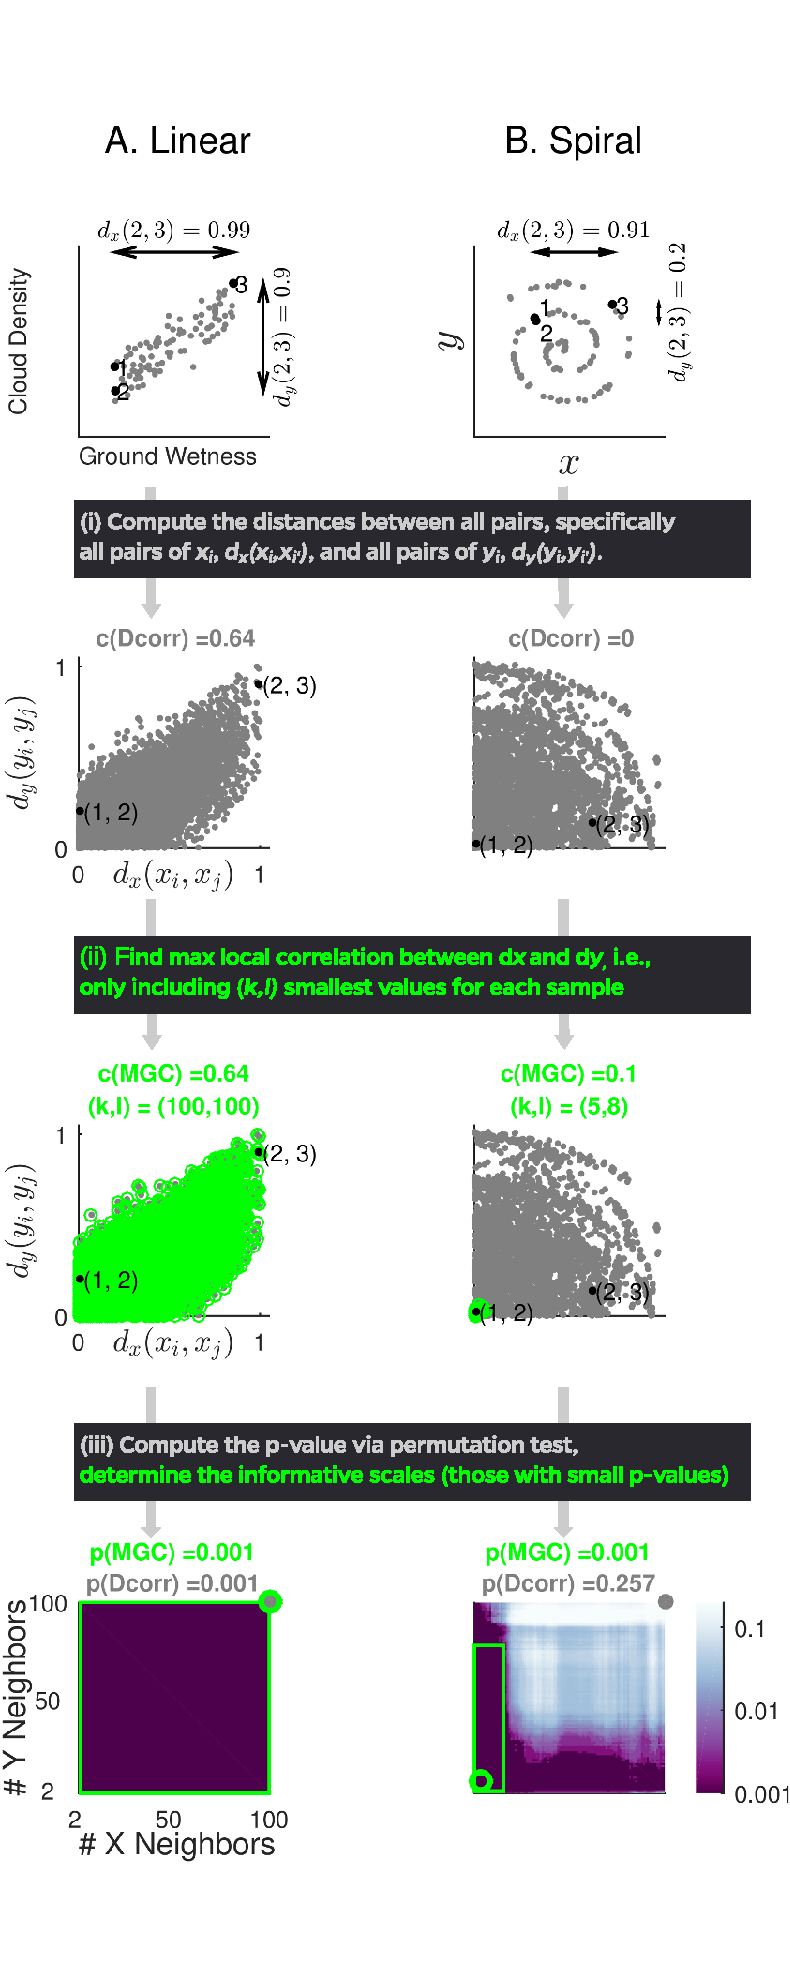
\includegraphics[height=0.9\textheight,trim={0cm 1.8cm 0 2cm},clip]{Figures/Fig1Allb.pdf}
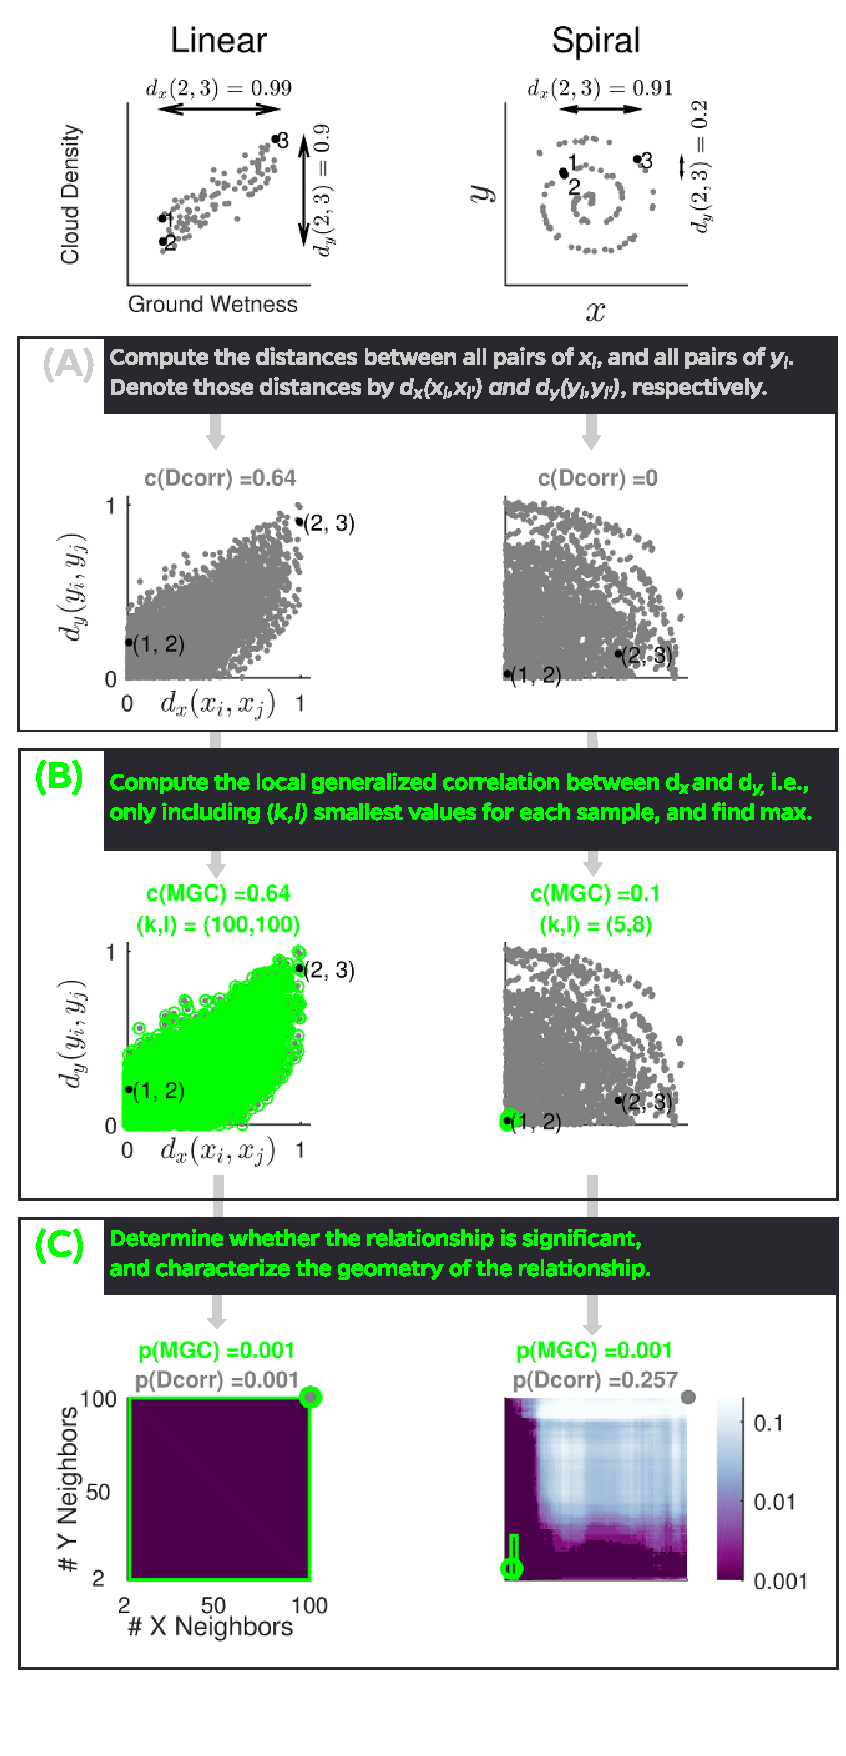
\includegraphics[width=0.5\linewidth]{Figures/Fig1All}
\caption{
Illustration of the three steps of Multiscale Generalized Correlation (\Mgc)  using  $50$ pairs of cloud density ($x_i$) and grass wetness ($y_i$).
We present two different relationships:  linear (left column) and nonlinear spiral  (right column; see Appendix \ref{appen:function} for simulation details).
Insights into the data available only from running \Mgc~are highlighted in {\color{green}green.} Results using \Dcorr~\cite{SzekelyRizzo2009}, a state-of-the-art dependence test that \Mgc~extends, are shown for comparative purposes.
%
Samples $1$, $2$, and $3$ (black) indicate how \Mgc~is able to discover nonlinear relationships (arrows in the scatterplots above section A show $x$ distances and $y$ distances between points 2 and 3).
The three steps of \Mgc~are:
%
\textbf{(A)} Compute all distance pairs. Distances are linearly correlated in the linear relationship, whereas they are not in the spiral relationship, as indicated by \Dcorr's test statistic, $c(\Dcorr)$ (in the title of each plot).  \Dcorr~uses all distances (gray dots) to compute its test statistic and p-value, whereas \Mgc~uses only the local distances (green dots) whose scale is chosen in the next step.
%
\textbf{(B)} Compute all local generalized correlations $c^{kl}$ between $x$ distances and $y$ distances, and find the maximum (after smoothing).
The scale with maximum local generalized correlation (after smoothing) is the global scale for the linear relationship, whereas the maximum is a very local scale for the spiral relationship. The heatmaps show the joint distance matrix $\{c_{ij}\}$ at the optimal scale (titles state the maximum local generalized correlation $\GG(\Mgc)$, and the scales that achieve it).
\textbf{(C)}
Determine whether the relationship is significantly dependent, and characterize the geometry of the relationship.
The heatmap shows the local  significance values for all scales (computed via a permutation test). The green circle indicates the scale with maximum local generalized correlation (from step (B));  the estimated optimal scales are all scales within the green rectangle, which is the largest rectangle whose elements all have large local statistics with small significance values. The global scale (gray dot) is always in the top right corner, regardless of the data.
Titles state the p-values,  $p(\Mgc)$~and $p(\Dcorr)$.
Thus, only \Mgc~infers that local scales are important in the spiral relationship, indicating strong nonlinearities in the relationship,
 and also demonstrating that global scales are important in the linear relationship,  thereby uniquely detecting dependence and characterizing the geometry in both relationships.
}
\label{f:newschem}
\end{SCfigure}

The key, therefore, to successfully determining the presence and geometry of a relationship is to adaptively estimate the number of neighbors that are particularly informative.
This is especially important in high-dimensional data, where simple visualizations do not reveal the relationships to the unaided human eye.
Our methodology---called ``Multiscale Generalized Correlation'' (\Mgc)---extends essentially all previously proposed pairwise comparison-based approaches to enable estimation of the  optimal scales.
Crucially, \Mgc~adaptively estimates the informative scales for any relationship---linear or nonlinear, low-dimensional or high-dimensional, unstructured or structured---in a computationally efficient and statistically consistent fashion, therefore guaranteeing equally good or better  statistical performance compared to existing global methods in any setting.
Moreover, the estimated scales are informative about the geometry of the dependence structure, therefore providing further guidance for subsequent experimental or analytical steps. \Mgc~is thus a hypothesis-testing and geometry-characterizing methodology that builds on recent developments in manifold learning (operating on pairwise comparisons) by combining them with complementary developments in harmonic (multiscale) analysis.
It is this union of three disparate disciplines spanning data science that enables improved theoretical and empirical performance.

The first step of \Mgc~is the same as essentially all other nonparametric dependency tests:
compute the Euclidean distances between all pairs of one property {(e.g., $a_{ij}=|x_i-x_j|$ for cloud densities)} and the corresponding Euclidean distances between all pairs of the other property {(e.g., $b_{ij}=|y_i - y_j|$ for grass wetnesses;} see Figure \ref{f:newschem}{\color{magenta}A}.
The ``joint distance'' for any pair across both properties is the product of the centered distances for each property $c_{ij}=(a_{ij}-\bar{a}) \times (b_{ij}-\bar{b})$.
% , and $C$ is the $n \times n$ matrix of joint distances.}
Global methods, such as \Dcorr, then compute the ``generalized correlation'', which is simply the normalized sum of the joint distances, $\mh{c}= \frac{1}{z}\sum_{i,j} c_{ij}$, where $z$ normalizes $\mh{c}$ to be between $-1$ and $1$ (see Appendix \ref{appen:global} for details on the global methods and different centering schemes).
\Mgc~instead computes the set of  ``local generalized correlations''.
% for all scales, to find the best one.
A local generalized correlation is the generalized correlation that only includes the $k$ smallest distances for each $x_i$, and the $l$ smallest distances for each  $y_i$.
\Mgc~computes these local generalized correlations for all possible scales $k$ and $l$, incrementally increasing the number of neighbors $k$ for each $x_i$, and separately increasing the number of neighbors $l$ for each $y_i$.
The \Mgc~\emph{test statistic} is the local generalized correlation with the best scale, that is, the scales $(k,l)$  whose local generalized correlation is largest after smoothing (\Mgc~smooths to address noisy samples; see  Appendix  \ref{appen:mgc} for details on \Mgc).
Figure \ref{f:newschem}{\color{magenta}B} shows the joint local distances  for the $(k,l)$ pair chosen by \Mgc~for these simulations (that is, only keeping the $k$ and $l$ closest distances for each sample).
The green circles in Figure \ref{f:newschem}{\color{magenta}A} show the set of distances amongst the $(k,l)$ nearest neighbors that \Mgc~selected for these particular simulations.
For the linear case, all the neighbors are used, whereas for the nonlinear case, only the relatively local pairs are used.
These two examples  illustrate that \Mgc~is adapting to the differing geometries of the two cases.

The third and final step is to determine whether the relationship is significantly dependent, and characterize the geometry of that relationship (Figure \ref{f:newschem}{\color{magenta}C}).
\Mgc~determines the significance of the relationship via a permutation test.
Specifically, \Mgc~permutes the labels of either the $x_i$'s or the $y_i$'s, and computes the maximum local generalized correlation and its scales.
By repeating this process many times, \Mgc~estimates the null distribution of the test statistic, which it then uses to compute the p-value.
This procedure sidesteps the multiple hypothesis testing problem  by only computing the p-value for the scale with the maximum local generalized correlation (after smoothing), ensuring that \Mgc~is a valid and unbiased test (meaning that false positive rate is properly controlled at the specified type I error rate; see Appendix \ref{appen:algorithms} for details).
The procedure also computes ``local significance values''  for each $(k,l)$ scale.  The multiscale significance map is the set of all of these significances, and provides a principled yet pictorial representation of the geometry of the relationship.
% \todo{but here, by “geometry”, do you mean like spiral vs. linear, or instead “the range of spatial scales at which there is signal/structure”.  it sounds like you are implying the former, whereas the latter seems like what i think you are really saying.}
The estimated optimal scales (green boxes) are all the scales within the largest rectangle that includes local significance values that are all no larger than the p-value of \Mgc.
For the linear example, the global scale (\Dcorr's) yields low significance values, implying a nearly linear relationship.
On the other hand, for the nonlinear relationship, only a set of small local scales yields low significance values, implying a strong nonlinear relationship that is undetected by \Dcorr~but revealed by \Mgc.
These illustrations  demonstrate that \Mgc~detects dependence in both linear and spiral relationships, and characterizes the geometry underlying each by providing multiscale significance maps that indicate which scales encode dependence for the given dataset.

Running \Mgc~is straightforward---it requires inputting $n$ samples of two measured properties.
Our open source implementation\footnotemark\footnotetext{In both MATLAB and R from our website, \website.} requires about the same running  time complexity as conventional methods, situating it to be useful in a wide variety of contexts.
The following sections document \Mgc's empirical, computational, and theoretical properties; \Mgc~pseudocode are provided in Appendix~\ref{appen:algorithms}.
% Mathematical details of prior global methods are provided in Appendix \ref{appen:global},
% details for \Mgc~are provided in Appendix \ref{appen:mgc}, and \Mgc~pseudocodes are provided in Appendix~\ref{appen:algorithms}.

\begin{figure}[!ht]
\centering
% \subfigure{
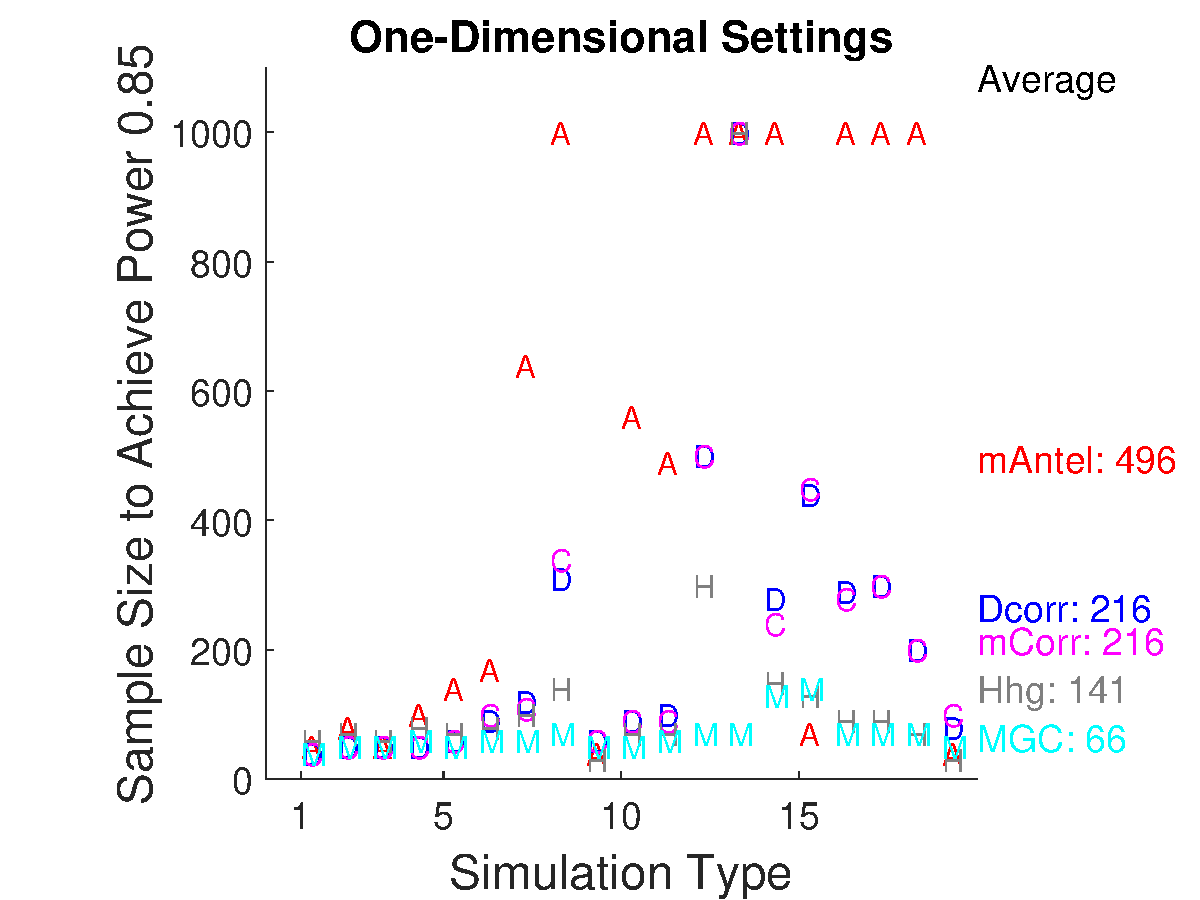
\includegraphics[width=0.48\textwidth,trim={1.5cm 0 0cm 0cm},clip]{Figures/Fig1DPowerSummarySize}
% }
% \subfigure{
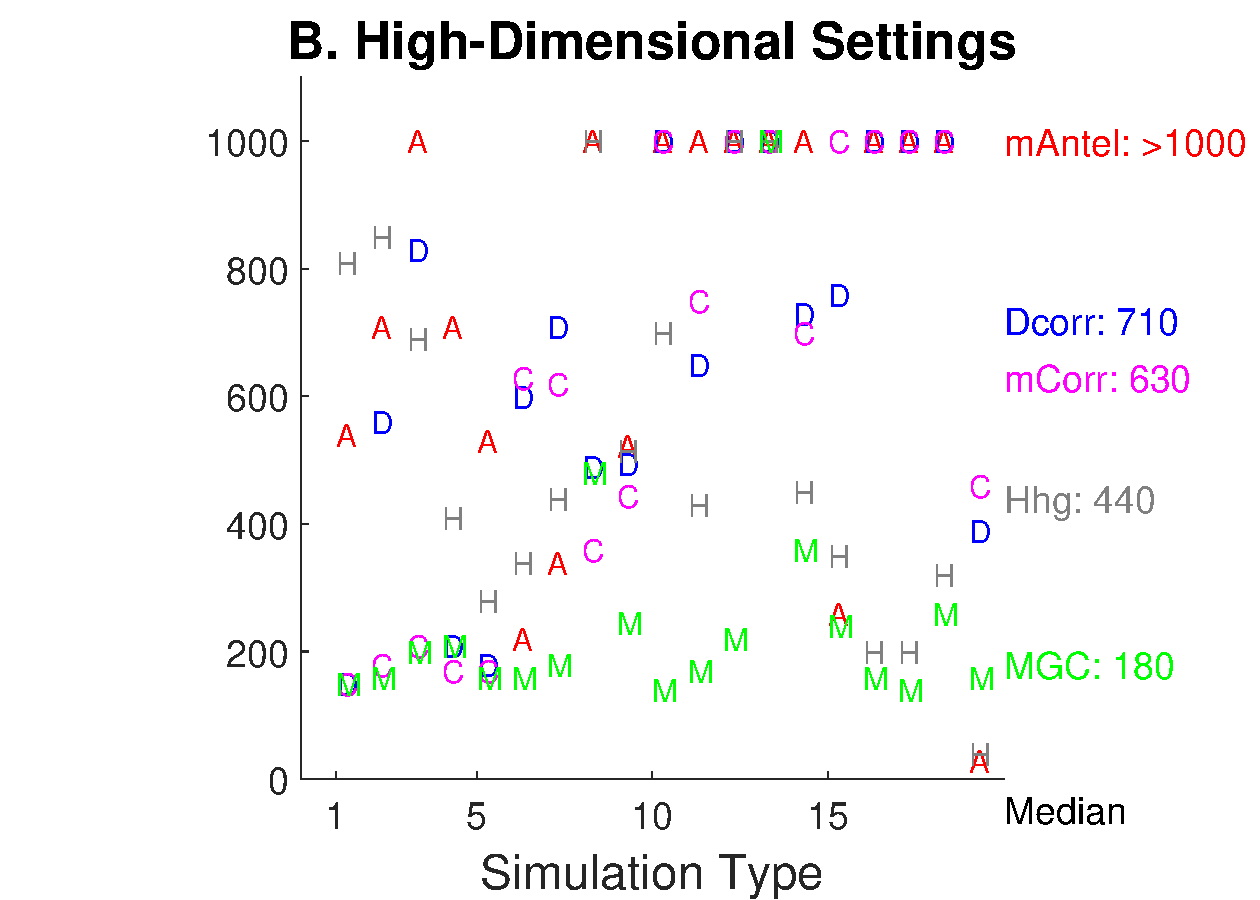
\includegraphics[width=0.48\textwidth,trim={1.5cm 0 0cm 0cm},clip]{Figures/FigHDPowerSummarySize}
% }
  \caption{
Sample size of different methods to achieve a power of $85\%$ at type 1 error level $0.05$, for the $20$ different relationships including both one-dimensional \textbf{(A)} and high-dimensional \textbf{(B)} relationships.
The x-axis is the simulation type, and the y-axis shows the minimal sample size of each method to achieve $85\%$ testing power, the smaller the better.
For panel (A), the dimension is fixed at $1$ for each relationship,
% and the minimal size to achieve the required testing power is estimated.
and for panel (B), the dimension for each relationship is chosen on the basis of the experiments in Supplementary Figure~\ref{f:nDAll}.
% https://www.ncbi.nlm.nih.gov/pmc/articles/PMC3826013/.
The sample size always increments by $10$ and is bounded by $1000$ in the experiment, with the median sample size for each method reported in the far right column. The results indicate that \Mgc~is a superior choice for finite-sample dependency testing; for example,  the second best method (\Hhg) requires nearly two and a half times the sample size of \Mgc~to achieve the same median power across high-dimensional settings.}
\label{f:Summary}
\end{figure}

\subsection*{\Mgc~Requires Substantially Fewer Samples to Achieve the Same Power Across Essentially All Dependencies and Dimensions}

When, and to what extent, does \Mgc~outperform other approaches, and when does it not?
To address this question, we formally pose the following hypothesis test (see Appendix \ref{appen:global} for details):
\begin{align*}
H_0\!:& \; x \text{ and } y \text{ are independent} \\
H_A\!:& \; x \text{ and } y \text{ are \emph{not} independent}.
\end{align*}
The standard criterion for evaluating statistical tests is to compute the probability that it correctly rejects a false null hypothesis, i.e. the testing power at a given type 1 error level.
We compare \Mgc~with four state-of-the-art tests:
(i) \Mantel, which is widely and successfully used in biology and ecology \cite{Mantel1967},
(ii) \Dcorr, as discussed above,
(iii) \Mcorr, a modified version of \Dcorr~designed to be unbiased for sample data \cite{SzekelyRizzo2013a}, and
(iv) \Hhg, a distance-based test that is very powerful for detecting low-dimensional nonlinear relationships \cite{HellerGorfine2013}.
The latter three have theoretical support guaranteeing that they will detect any dependence with enough samples, whereas \Mantel~has no such theoretical guarantee indicating when it should not work.
We consider $20$ different noisy dependence relationships, most taken from the existing literature, including  ``monotonic'' %nearly linear
($1-5$), strongly nonlinear ($6-19$), and independent ($20$) relationships \cite{SzekelyRizzoBakirov2007, SimonTibshirani2012, GorfineHellerHeller2012, HellerGorfine2013, SzekelyRizzo2013a}.
Function details are in Appendix~\ref{appen:function}, with additional supporting figures in Appendix~\ref{appen:figs}.
 The visualization of one-dimensional noise-free (black) and noisy (gray) samples is shown in Supplementary Figure~\ref{f:dependencies}
(note that the ``monotonic'' functions are only monotonic in one-dimension).

For each relationship, we compute the sample size required to achieve $85\%$ power for both a one-dimensional scenario and a high-dimensional scenario. The high-dimensional relationships are more difficult because each dimension is designed to have less and less signal, 	so there are many noisy dimensions, and they cannot easily be visualized.
Figure~\ref{f:Summary} demonstrates that for essentially all relationships in both low and high dimensions, \Mgc~requires far fewer samples to achieve high power.  The far right of each panel indicates the median sample size required over all $20$ relationships.
For the one-dimensional cases, \Mgc~only requires a median 60 samples, whereas the next best approach requires a median of 80 samples, 33\% more than \Mgc.
For the high-dimensional cases, \Mgc~only requires a median of 180 samples, whereas the next best approach requires a median of 440 samples, nearly 250\% more samples.
Supplementary Figures \ref{f:nDAll} and \ref{f:1DAll} further explore the relationship between power, sample size, and dimensionality for the different tests, including several  variants of \Mgc.
For nearly every relationship {and dimensionality}, \Mgc~requires substantially fewer samples than competing methods to achieve the same or higher power.
Stated another way, at a fixed sample size of $100$, compared to \Mgc, other methods only achieve between $15\%$ and $81\%$ average power in the one-dimensional relationships, and between $26\%$ and $58\%$ power in the high-dimensional relationships (see Supplementary Figure \ref{f:Summary2} for details).

\subsection*{\Mgc~Characterizes the Geometry of Dependence}
\label{main3}

\begin{figure}[!ht]
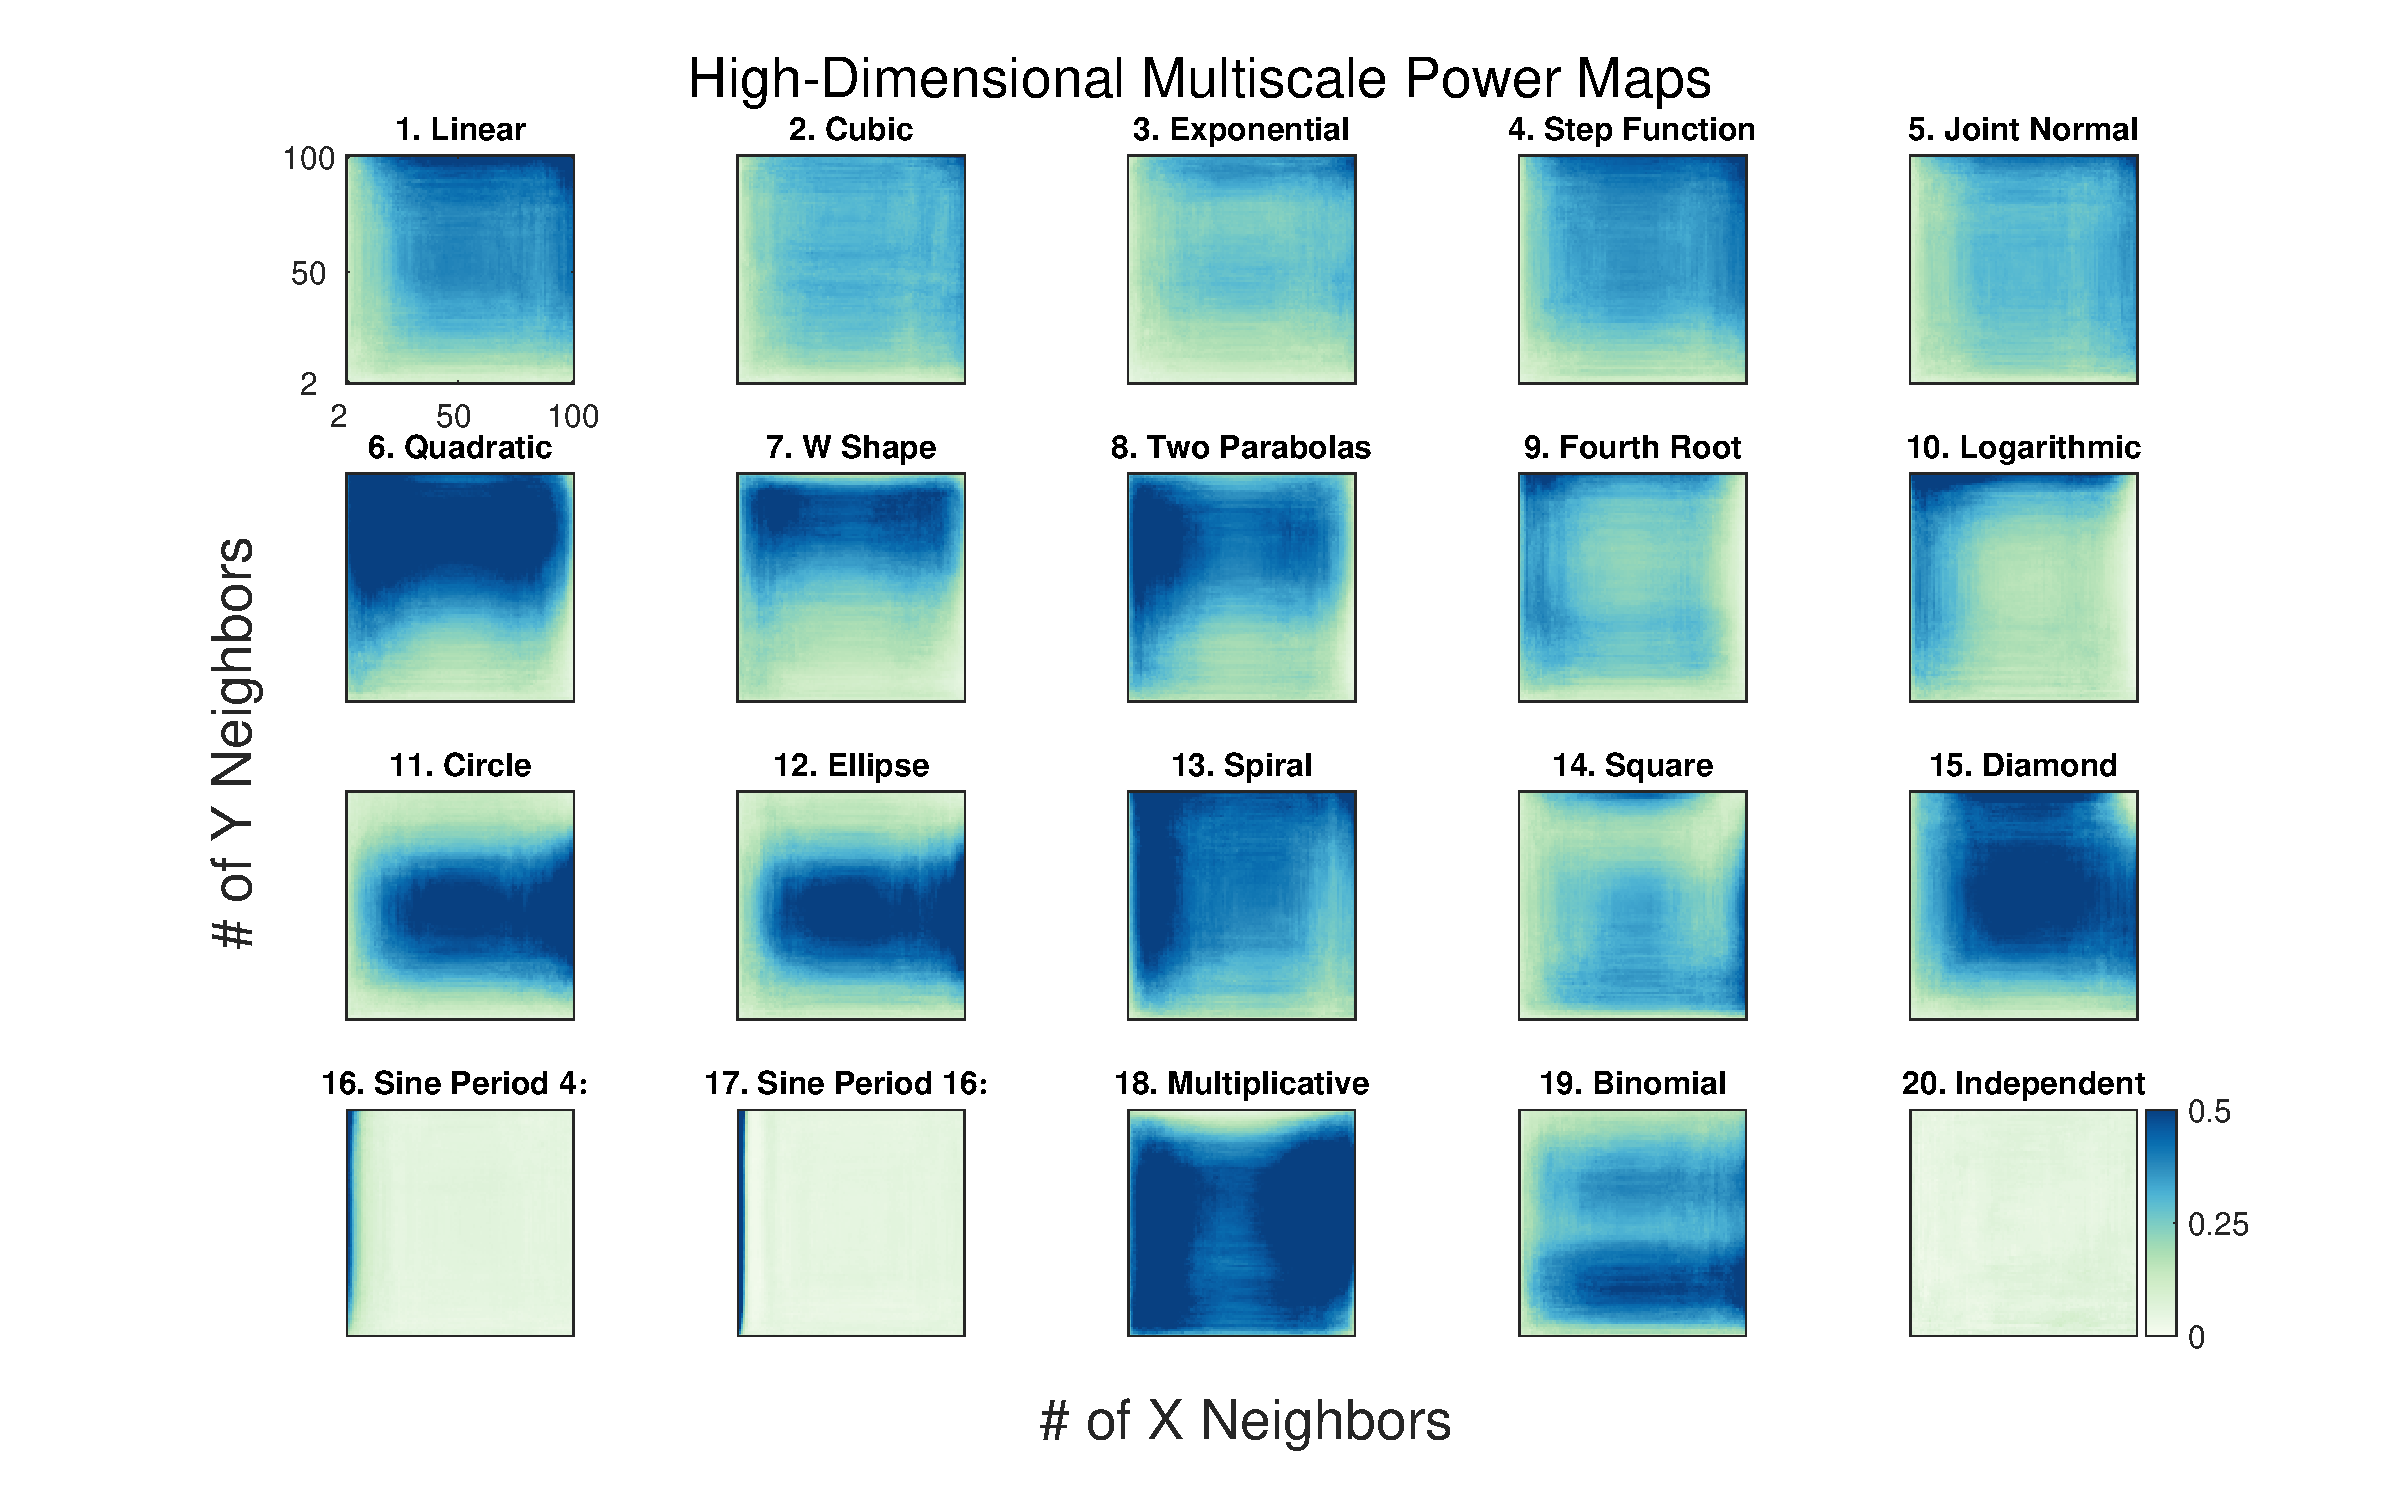
\includegraphics[width=1.0\textwidth,trim={3cm 0.5cm 1.8cm 0.5cm},clip]{Figures/FigHDHeat}
\caption{Multiscale Power Maps allow \Mgc~to determine the geometry of the dependence function.
For each of the 20 panels, the abscissa and ordinate denote the number of neighbors for $X$ and  $Y$, respectively, and the color denotes the power at that scale. For each simulation, the sample size is $100$,  and the dimension is determined by the largest dimension for \Mgc~to have power exceeding $0.5$ at significance level $0.05$. Each simulation yields a different multiscale power map characterizing the geometry of dependence.
For example, the global scale (not shown because it  is always in the top right corner) is optimal only for nearly linear dependencies, i.e. the plots in the top row.
For each panel, the green dot and rectangle show the scale with the maximum test statistic,  and the estimated optimal scales, estimated from a single trial. Note that the estimated optimal scales tend to be near the most powerful scales.
}
\label{f:powermaps}
\end{figure}

Often, investigators desire to understand more than whether a relationship exists, but also the geometry of that relationship, to provide insight or guide further experimentation.
A single scalar quantity (such as effect size) is inadequate given the vastness and complexities of possible geometries, while \Mgc~provides a simple, intuitive, and nonparametric (and therefore infinitely flexible) description of the geometry of any relationship.

The \emph{multiscale power map} is an image that shows, for a given dependence relationship, the power as a function of the scales of $x$ and $y$.
Figure~\ref{f:powermaps} provides the multiscale power maps for all 20 different high-dimensional relationships, illustrating how the power of local generalized correlations changes with  neighborhood size.
For the ``monotonic'' dependencies (1-5), the best neighborhood choice always includes the largest scale, i.e., the global one.
Moreover, the multiscale power maps for monotonic cases are all qualitatively similar.  This suggests that the signature of a monotonic relationship is a multiscale power map whose power is increasing as we increase both scales, regardless of its details or dimensionality.
For all nonlinear/non-monotonic dependencies (6-19),  \Mgc~chooses smaller scales for $x$ or $y$. Thus, a global optimal scale implies a ``monotonic'' dependency, otherwise the dependency is strongly non-monotonic.
Furthermore, similar dependencies have similar local generalized correlation structures, and thus, similar multiscale power maps. For example, logarithmic (10) and fourth root (11), though very different functions analytically, are geometrically similar, and yield very similar power maps.
Similarly,  (12) and (13) are trigonometric functions, and they share a narrow range of significant local generalized correlations.
Both circle (16) and ellipse (17), as well as square (14) and diamond (18), are closely related geometrically, and have similar power maps.
These maps therefore characterize the geometry of these relationships, differentiating different dependence structures, which can have important implications for and assist subsequent analysis steps.


Power map generation requires knowledge of the true distribution of the data, which is unavailable for real data.
Thus, for real data, \Mgc~computes (i) a multiscale correlation map  (akin to a multiscale power map), from which it estimates the (ii) maximum local generalized correlation, and (iii) the optimal scales.  The maps are noisy because they utilize noisy samples, rather than the true distribution, to obtain their values.  Nonetheless, they provide estimates of the  the maximum local generalized correlation  and optimal scales, thereby improving power and providing information about the geometry of the relationship.
In Figure \ref{f:powermaps} we superimposed the estimated maximum local generalized correlation (green dots) and optimal scales (green boxes) from a single trial onto the power maps that were constructed from averaging 100 trials.
 % The green dots in Figure \ref{f:powermaps} indicate the scale of maximum local generalized correlation for a single trial, and the green boxes indicate the estimated optimal scales from that trial.  These have been superimposed on the power map for comparison.
 In every case the estimated optimal scales are either very close to or exactly the same as the true optimal scales, indicating that \Mgc~can often correctly estimate the true optimal scales in practice.

\subsection*{\Mgc~Theoretically Dominates its Global Counterparts {by Always Achieving a Given Power with Fewer (or the same number of) Samples}}
\label{s:theory}

``Oracle \Mgc'' is a version of \Mgc~that uses the true distribution of the data to accurately select the optimal local generalized correlation, rather than estimating it from the data (see Appendix~\ref{appen:mgc2} for details). More specifically, Oracle \Mgc~selects the scale that maximizes power, whereas ``Sample \Mgc'' selects the scale that maximizes the smoothed test statistic.
In either case,  \Mgc~can generalize any distance-based dependence test by restricting it to only consider local distances.  Any global test that \Mgc~generalizes is called \Mgc's ``global counterpart''.  The main theoretical result we obtain is as follows:
%
\begin{thm} \label{t:dominate}
Oracle \Mgc~statistically dominates its global counterpart.
% Thus, no matter which dependence function, dimensionality, and sample size, Oracle \Mgc~achieves equal or higher power than its global counterparts for any global correlation.
Thus, no matter which dependence function, dimensionality, and type I error level, Oracle \Mgc~requires fewer (or an equal number of) samples to achieve a given power, compared to its global counterpart.
%
More precisely, in \emph{linear} relationships, Oracle \Mgc~requires the same number of samples to achieve power of the global test, and in various nonlinear and non-monotonic relationships, Oracle \Mgc~requires far fewer samples to achieve the same power of the global counterpart.
%
\end{thm}

The above result follows immediately from Theorems \ref{t:thm1}, \ref{t:linear}, and \ref{t:non}, which are described in Appendix \ref{appen:theory}. In short, the dominance theorem follows from demonstrating that \Mgc~achieves higher power for even a simple quadratic function, suggesting that \Mgc~dominates for higher order polynomial dependence functions (and therefore potentially many nonlinear functions).
Empirically, Sample \Mgc~performs very closely to Oracle \Mgc~in most simulated relationships (see Supplementary Figures \ref{f:nDAll} and \ref{f:1DAll}), suggesting that Sample \Mgc~may also dominate global methods with high probability.

Finally, though a na\"ive implementation of \Mgc~requires $\mc{O}(n^4)$ operations, we have devised a serial implementation that requires only $\mc{O}(n^2 \log n)$.  Assuming access to parallel computation, for example on modern multi-core architecture such as on laptops, mobile phones, and workstations, \Mgc~requires only $\mc{O}(n^2 \log n / T)$ operations, where $T$ is the number of parallel threads (see Algorithm \ref{alg:all_scales} for details).  Since $T$ is often larger than $\log n$, in practice, \Mgc~is actually $\mc{O}(n^2)$, and a constant factor slower than its global counterpart.  For example, when $n=5000$, \Mcorr~requires $0.5$ seconds to compute the test statistic, whereas its \Mgc~requires $5$ seconds. Obviously, the cost and time to obtain $2.5 \times$ more data far exceeds a few seconds.


% Moreover, Algorithm \ref{alg:all_scales} achieves this dominance with merely an additional multiplicative computational cost of $\log n$, rather than an additional $n^2$ that would result from a na\"ive implementation.
% \new{Finally, though \Mgc~is minimally more computationally expensive than global methods, the cost of collecting $2.5 \times$ more data typically \emph{far} outweighs the cost of waiting a few more minutes for the results.}

\subsection*{\Mgc~Discovers {the Geometry and} Relationships in Real Data Examples}
\label{numer3}



\begin{figure}[!ht]
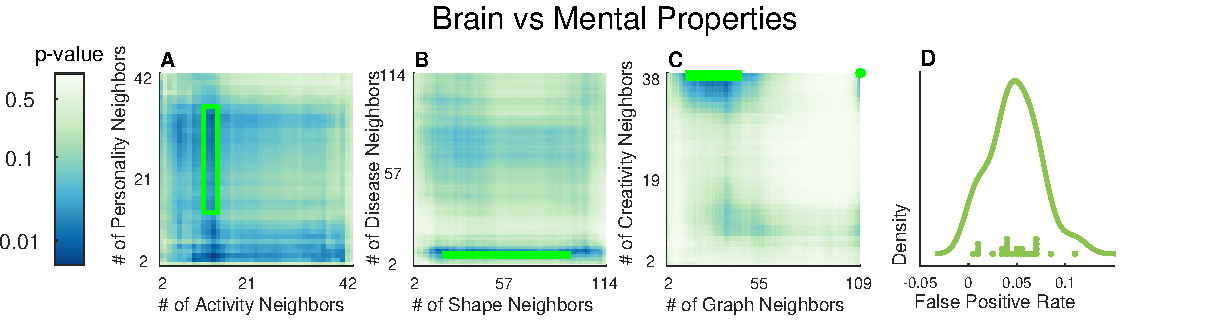
\includegraphics[width=1.0\textwidth,trim={2cm 0 1cm 0},clip]{Figures/FigReal}
\caption{In real data, \Mgc~discovers the geometry and dependence when they exist, and does not detect dependence when it does not exist.  \textbf{(A)} Multiscale significance maps and the estimated optimal scales for two different experiments between brain and mental properties: in \textbf{(Ai)}, only local scales are significant for testing brain activity vs the five-factor personality model (42 subjects), suggesting that the relationship is strongly nonlinear, whereas in \textbf{(Aii)} the global scale is optimal for testing brain networks vs creativity (114 subjects), suggesting a linear relationship.
%
\textbf{(B)} \Mgc~provides new insights for discovering imaging biomarkers between brain shape and depression (109 subjects): \textbf{(Bi)} Joint distance matrix that \Mgc~uses to quantify the structure of dependence; only a local test reveals a significant dependence.
\textbf{(Bii)} The distributions of within-class and between-class distances for high-risk people (class two), demonstrating that within-class differences are sometimes \emph{larger} than between-class distances for the high-risk population, a counterintuitive insight into the geometry of the dependence only gleaned by \Mgc.
\textbf{(C)} Screening performance of \Mgc~for two different contexts: \textbf{(Ci)} Cancer biomarker discovery \cite{Wang2017} and \textbf{(Cii)} Neuroimaging false postive rate confirmation \cite{Eklund2015}.
\textbf{(Ci)}  compares the p-values for screening peptides to identify potential biomarkers for pancreatic cancer. The horizontal-axis corresponds to the p-values of testing each biomarker between pancreatic cancer patients versus normal people, and the vertical-axis is for the p-values of testing between pancreatic cancer patients versus all other subjects (including normal people and patients with three other cancer types). \Mgc~succesfully and uniquely identifies a potentially useful biomarker for pancreatic cancer, out of $318$ proteins from $98$ subjects.
\textbf{(Cii)} demonstrates that \Mgc~is a valid test that does not inflate the false positives in screening and variable selection. It plots the density estimate for the false positive rates of applying \Mgc~to screening / select the ``falsely significant" brain regions versus  independent noise experiments; dots indicate the false positive rate of each experiment. The mean $\pm$ standard deviation is $0.0538 \pm 0.0394$.}
\label{f:real}
\end{figure}

% \Mgc~can be applied to real data scenarios with complex structures, provided appropriate distance measures are available. We apply \Mgc~to three different scenarios: (i) brain activity versus personality, (ii) brain shape versus depression, and (iii) brain networks versus creativity.  For each comparison, we chose appropriate distances for both kinds of data (see Appendix \ref{appen:real} for details), and ran \Mgc~to obtain both a p-value and a multiscale significance map, akin to the multiscale power maps shown above.

The above theory and simulated experiments motivated us to test \Mgc~on five different applications: two relating brain properties and mental properties, one discovering imaging biomarkers for cognitive decline, one discovering proteomics biomarkers for cancer diagnostics, and another demonstrating that \Mgc~does not suffer from false positive inflation.

\begin{table*}[!ht]
\centering
\caption{The p-values for the first three real data experiments. \Mgc~is the only method that \emph{always} uncovers the existence of significant relationships and the only method that \emph{ever} discovers the underlying optimal scales. Bold indicates lowest p-value per dataset.}
\label{t:real}%
\begin{tabular}{|c||c|c|c|c|c|}
\hline
Testing Pairs / Methods & Sample \Mgc & \Mantel & \Dcorr & \Mcorr & \Hhg \\
\hline
Activity vs Personality & $\textbf{0.049}$  & $0.990$ & $0.663$ & $0.447$ & $0.056$ \\
\hline
Network vs Creativity & $\textbf{0.013}$  & ${0.010}$ & $\textbf{0.010}$ & $\textbf{0.013}$ & ${0.029}$ \\
\hline
Shape vs Disease & $\textbf{0.029}$  & $0.080$ & $0.108$ & $0.112$ & $0.161$ \\
\hline
\end{tabular}
\end{table*}



\subsubsection*{\Mgc~Reveals the Latent Geometry between Brain and Mental Properties}

% The study of the relationship between our physical and psychological properties dates back at least to the Greeks, if not further.  Neuroscientists, neurologists, psychiatrists, cognitive scientists, and even machine learning professionals seek to understand how the brain gives rise to the richness of the human experience.
Here we investigate two particularly interesting properties of the human psyche: personality and creativity.  Both have been extensively studied, yielding quantitative metrics for evaluating them using structured interviews \cite{Costa1992,Jung2009}.  We utilized two previously published datasets, to determine whether \Mgc~could yield insight into the relationship between our brains and these mental properties.

First, we investigated the relationship between resting-state functional  magnetic resonance activity (rs-fMRI) activity and personality \cite{AdelsteinEtAl2011} (see Appendix \ref{app:personality} for details).
Figure \ref{f:real}{\color{magenta}Ai} shows that many local scales yield significant p-values ($< 0.05$), whereas the global scale fails to detect this significant dependence. In fact, all previously proposed global dependence tests under consideration (\Mantel, \Dcorr, \Mcorr, or \Hhg) fail to detect dependence at a significance level of $0.05$ (see Table \ref{t:real}), and only \Mgc~characterizes the geometry of the dependence.
Interestingly, the multiscale significance map does not look like any of the 20 maps from the simulated data, suggesting that the nonlinearity characterizing this dependency is more complex or otherwise different from those we have considered so far.

Second, we investigated the relationship between diffusion MRI derived connectivity and creativity \cite{Jung2009}  (see Appendix \ref{app:creativity} for details).
Figure \ref{f:real}{\color{magenta}Aii} and Table \ref{t:real} show that \Mgc~at the global scale can ascertain the dependency between the whole brain network and the subject's creativity (so are other global methods),
and further suggest a linear relationship and relatively little to gain by pursuing nonlinear regression techniques.
We therefore investigated the prediction of creativity using linear methods, but determined that the sample size was too low to obtain significant results (not shown).
This experiment demonstrates that for high-dimensional structured data with low sample sizes, only \Mgc~can  reveal a  linear dependence without having to resort to parametric techniques or  estimating a regression function, which requires a larger sample size.

\subsubsection*{\Mgc~for Discovering Imaging Biomarkers}

Imaging biomarkers are one of the most important tools in modern medicine, for prognostics, diagnostics, surgery planning, and more \cite{Prescott2013}. The more sensitive a test, the better.  Given \Mgc's superior power over other global tests, we investigated whether \Mgc~could detect a dependence between brain shape and disease status: non-affected, high-risk, or clinically depressed (see Appendix \ref{app:depression}) \cite{ParkEtAl2008,PosenerEtAl2003}.
Only \Mgc~was able to detect a dependence between brain shape and disease status, suggesting a local signal and a nonlinear geometry (Table \ref{t:real}).  Investigating further, we analyzed the matrix of local distances that \Mgc~utilizes to compute its p-value (Figure \ref{f:real}{\color{magenta}Bi}).  It seems from this matrix that the within-class distances can be \emph{larger} than the between-class distances.  Figure \ref{f:real}{\color{magenta}Bii} confirms that this is indeed the case for the high-risk individuals.  This counter-intuitive result indicates that high-risk individuals can have highly variable brain shapes that are more different from one another than they are from either non-affected or clinically depressed individuals.  This geometric characterization of the relationship between brain shape and disease was only discovered due to \Mgc.
% Figure \ref{f:real}{\color{magenta}C} shows the matrix of distances between all pairs of observations
% provides the significance map for testing whether the shape of the hippocampus in the right hemisphere is independent of disease status using \Mgc. Again, many local scales yield significant p-values indicating both the existence and geometry of a dependence, whereas none of the global methods even detect a significant dependence  (see Table \ref{t:real}).

\subsubsection*{\Mgc~for Proteomics Screening}

Screening proteomics data for biomarkers often involves the analysis of tens of thousands of proteins, peptides, or transcripts in multiple samples representing a variety of disease types. Determining whether there is a relationship between one or more of these markers and a particular disease state can be challenging, but is a necessary first step for subsequent analysis. We sought to discover new useful protein biomarkers from a quantitative proteomics technique that measures protein and peptide abundance called Selected Reaction Monitoring (SRM) \cite{PMID21248225} (see Appendix \ref{app:cancer} for detailed processing and full results).
Specifically, we were interested in finding biomarkers that were unique to pancreatic cancer, because it is lethal and no clinically useful biomarkers are currently available.

We obtained a dataset consisting  proteolytic peptides derived from the blood samples of  $98$ individuals harboring pancreatic ($n=12$), ovarian ($n=24$), colorectal cancer ($n=29$), and healthy controls  ($n=33$).
The processed data included $318$ peptides derived from $121$ proteins.
Previously, we used these data and other techniques to find ovarian cancer biomarkers (a much easier task because the dataset has twice as many ovarian patients) and validated them with subsequent experiments \cite{Wang2017}. Therefore, our first step was to check whether \Mgc~could correctly identify ovarian biomarkers. Indeed, the pepetides that have been validated previously are also identified by \Mgc (see Appendix \ref{app:cancer}).
Emboldened, using the same dataset,
we applied \Mgc~to screen for biomarkers unique to pancreatic cancer.  To do so, we first screened  for a difference between pancreatic cancer and healthy controls, identifying several potential biomarkers.  Then, we screened for a difference between pancreatic cancer and all other conditions, to find peptides that differentiate pancreatic cancer from all other subjects.
Among all methods, \Mgc~uniquely revealed one particular protein, neurogranin, that exhibited a strong nonlinear dependency with pancreatic cancer (Figure~\ref{f:real}{\color{magenta}Ci}).
Subsequent literature searches reveal that neurogranin is a potentially valuable biomarker for pancreatic cancer because it is exclusively expressed in brain tissue among normal tissues and has not been linked with any other cancer type.
\Hhg~identified neurogranin as well, but it also identified another gene that is likely to be a false positive based on literature evaluation. The rest of the global methods did not identify any new potential markers. Thus, \Mgc~alone identified the most likely biomarker for a debilitating disease without any false positives.
% Results such as this inspire more confidence (versus those that are suspect) and open a window for new experimental analysis.

\subsubsection*{\Mgc~Does Not Inflate False Positive Rates in Screening}

In the previous screening experiment, \Mgc~effectively selects the true positives in a cancer proteomics screening. In this final experiment, we empirically determine that \Mgc~does not inflate false positive rates via a neuroimaging screening.
% demonstrate that \Mgc~does not have high false negative rates, in the final experiment we empirically test whether \Mgc~inflates false positive rates.
To do so, we extend the work of Eklund et al. \cite{EklundKnutsson2012,Eklund2015},
where a number of parametric methods are shown to largely inflate the false positives. Specifically, we applied \Mgc~to test whether there is any dependency between brain voxel activities and random numbers (see Appendix \ref{app:noise} for details).
For each brain region, \Mgc~attempts to test the following hypothesis: Is activity of a  brain region independent of the time-varying stimuli?
Any region that is selected as significant is a false positive by definition in the screening process.  By testing each brain region separately, \Mgc~provides a distribution of false positive rates.  If \Mgc~is valid, the resulting distribution should be centered around the significance level, which is set at $0.05$ for these experiments.
%
We considered $25$ resting state fMRI experiments from the $1$,$000$ Functional Connectomes Project  consisting of a total of $1$,$583$ subjects \cite{biswal2010toward}.
Figure~\ref{f:real}{\color{magenta}Cii} shows the false positive rates of  \Mgc~for each dataset, which are centered around the critical level $0.05$, as it should be.
In contrast, many standard parametric methods for fMRI analysis, such as generalized linear models, can significantly increase the false positive rates, depending on the data and pre-processing details \cite{EklundKnutsson2012,Eklund2015}. Moreover, even the proposed solutions to those issues make linearity assumptions, thereby limiting detection to only a small subset of possible dependence functions.

\subsection*{Discussion}
\label{conclu}

We propose multiscale generalized correlation (\Mgc) to discover the presence and geometry of dependence across disparate types of data.
We proved that Oracle \Mgc~dominates global approaches in finite samples.  Specifically, comparing the number of samples required to achieve a given power for a fixed significance value, \Mgc~requires the same number as  global approaches on linear relationships, but far fewer than global approaches for strongly nonlinear relationships. We further empirically demonstrate via simulations that \Mgc~nearly always outperforms (requires fewer samples) global methods regardless of the dimension, sample size, and geometry.  Moreover, \Mgc~provides a map indicating which scales are maximally informative about the dependence structure.
In real data experiments, \Mgc~revealed dependency where global methods fail, as well as the geometry of those dependencies, and did not falsely detect signals when there were none.

\Mgc~also addresses a particularly vexing statistical problem that arises from the fact that methods for two subsequent statistical tasks are dissociated from one another: methods for determining whether two properties are related, and methods for determining how they are related.
The reason this dissociation creates a problem is that the statistical assumptions underlying the ``how related'' methods become compromised in the process of determining ``whether related'': this is the so-called ``post-selection inference'' problem \cite{berk2013valid}.
The most straightforward way to address this issue is to collect new data, which is costly and time-consuming. Therefore, researchers typically ignore this fact and make statistically invalid claims.
\Mgc~begins to get around this dilemma by carefully constructing its permutation test to estimate the scale in the process of determining a p-value, rather than after.
To our knowledge, \Mgc~is the first dependence test to take a step towards valid post-selection inference.

The fact that \Mgc~provides an estimate of the informative scales suggests several  theoretical steps to extend this work.
First, we could provide theoretical guidance for choosing the optimal scale in \emph{finite} samples, which could possibly further improve performance.  Second, because the multiscale significance maps provide insight into the geometry of dependence, we could theoretically determine a mapping from these maps to the set of all nonlinear functions to provide a formal characterization of the geometry of the dependency.

As a separate next theoretical extension, we could reduce the computational space and time required by \Mgc. \Mgc~currently requires space and time that are quadratic with respect to the number of samples, which can be costly for very large data.  Recent advances in related work suggest that we could reduce computational time to close to linear \cite{Huo2016}, although with some weakening of the theoretical guarantees \cite{zhang2017large}. Alternately, semi-external memory implementations would allow the running of \Mgc~on any data as long as the interpoint comparison matrix fits on disk rather than main memory \cite{Zheng2015,Zheng2016,Zheng2016c,Zheng2016b}. Another approach would be to derive an approximation to the asymptotic null distribution for \Mgc, obviating the need for the permutation test, but at the cost of potential finite-sample bias. %The fact that others have done so for kernel-based independence tests
%\cite{GrettonEtAl2005, GrettonGyorfi2010, GrettonEtAl2012}, which are equivalent to ``energy statistics'' (such as \Dcorr~and \Mcorr) \cite{SejdinovicEtAl2013, RamdasEtAl2015}, suggests that we could do so as well.

There are also a number of connections between \Mgc~and other prominent statistical procedures that may worth further exploration. First,  \Mgc~can be thought of as a regularized or sparsified variant of generalized correlation coefficients.  Regularization is central to high-dimensional and ill-posed problems, where dimensionality is larger than sample size. The connection made here between regularization and dependence testing opens the door towards considering other regularization techniques for correlation-based dependence testing, including \Hhg~and the approach described in Reshef et al. \cite{Reshef2011}. Second, \Mgc~can be thought of informally as  learning a metric.  We could therefore capitalize on the sub-specialty within machine learning and statistics called metric learning \cite{xing2003distance}.  In particular, deep learning  can be thought of as metric learning \cite{giryes2015deep}, and generative adversarial networks \cite{goodfellow2014generative} are implicitly testing for equality which is closely related to dependence.
While \Mgc~searches over a two-dimensional parameter space to optimize the metric, deep learning searches over a much larger parameter space, sometimes including millions of dimensions.  Probably neither is optimal, and somewhere between the two would be useful in many tasks.
Third, energy statistics provides state of the art approaches to other problems, including goodness-of-fit \cite{Szekely2005}, analysis of variance \cite{Rizzo2010}, conditional dependence  \cite{Szekely2014,Wang2015}, and feature selection \cite{LiZhongZhu2012,Zhong2015}, so \Mgc~can be adapted for them as well.
In fact, \Mgc~can also implement a two-sample (or generally the $K$-sample) test \cite{Szekely2004, heller2016consistent}; so further comparisons of \Mgc~to standard methods for two-sample testing will be interesting. Finally, although energy statistics have not yet been used for classification, regression, or dimensionality reduction, \Mgc~opens the door to these applications by providing guidance as to how to proceed.
Specifically, it is well documented in machine learning literature that the choice of kernel, metric, or scale often has an undesirably strong effect on the performance of different machine learning algorithms \cite{levina2004maximum}. \Mgc~provides a mechanism to estimate scale that is both theoretically justified and computationally efficient, by optimizing a metric for a task wherein the previous methods lacked a notion of optimization.  Nonlinear dimensionality reduction procedures, such as  Isomap \cite{TenenbaumSilvaLangford2000} and local linear embedding \cite{SaulRoweis2000} for example, must also choose a scale, but have no valid criteria for doing so.  \Mgc~could therefore be used to provide insight into multimodal dimensionality reduction as well.

Finally, \Mgc~is easy to use: it merely requires pairs of samples to run, and all the code is available in both R and MATLAB from \url{https://neurodata.io/tools/MGC/}, as well as the code to fully reproduce all the figures in this manuscript.  That \Mgc~is open source and reproducible, coupled with its empirical and theoretical dominance, situates \Mgc~to be useful in a wide range of applications.  We showed its value in  diverse applications spanning neuroscience  which motivated this work, and an 'omics example. Applications in other domains, extending beyond science even, to include finance, pharmaceuticals, commerce, and security, face similar questions of dependence and thus could likewise benefit from the methodology proposed here.

\clearpage
\pagestyle{empty}
\bibliographystyle{nature}
\bibliography{MGCbib}


\section*{Acknowledgment}
% \addcontentsline{toc}{section}{Acknowledgment}
This work was partially supported by
the Child Mind Institute Endeavor Scientist Program,
%
the National Science Foundation Division of Mathematical Sciences award DMS-1712947,
%
the National Security Science and Engineering Faculty Fellowship (NSSEFF),
%
the Johns Hopkins University Human Language Technology Center of Excellence (JHU HLT COE),
%
the Defense Advanced Research Projects Agency's (DARPA) SIMPLEX program through SPAWAR contract N66001-15-C-4041,
%
the XDATA program of DARPA administered through Air Force Research Laboratory contract FA8750-12-2-0303,
%
the Office of Naval Research contract N00014-12-1-0601,
%
the Air Force Office of Scientific Research contract FA9550-14-1-0033.
%
The authors thank Dr. Brett Mensh of Optimize Science for acting as our intellectual consigliere, and Dr.~Ruth Heller, Dr.~Bert Vogelstein,  and Dr.~Yakir Reshef for insightful suggestions.

\clearpage
\appendix
\setcounter{figure}{0}
\renewcommand{\thealgorithm}{C\arabic{algorithm}}
\renewcommand{\thefigure}{E\arabic{figure}}
\renewcommand{\thesubsection}{\thesection.\Roman{subsection}}
\renewcommand{\thesubsubsection}{\thesubsection.\arabic{subsubsection}}

\section{Global Methods for Testing Dependence}
\label{appen:global}
To better understand the multiscale generalized correlation, in this section we first formally state the testing scenario, followed by formalizing the notion of the generalized correlation coefficient and reviewing four existing dependence tests: the \Mantel~test, distance correlation (\Dcorr), modified distance correlation (\Mcorr), and \Hhg. They are arguably the most popular and well-known statistical tests for dependence, and serve as the benchmarks in this paper. Note that the first three are conventional correlation measures, which can be used for building up local generalized correlations and thus \Mgc.

\subsection{Testing Independence}

A theoretical investigation of the performance of any dependence test requires formalizing the statistical hypotheses.
 Given pairs of observations $(\mb{x}_{i},\mb{y}_{i}) \in \Real^{D} \times \Real^{D_y}$ for $i=1,\ldots,n$, assume they are independently identically distributed as $(\mbx,\mby) \iid f_{xy}$. If the two random variables \mbx~and \mby~are independent, the joint distribution equals the product of the marginals, i.e., $f_{xy}=f_x f_y$.  The statistical hypotheses for testing independence is as follows:
\begin{align*}
& H_{0}: f_{xy}=f_{x}f_{y},\\
& H_{A}: f_{xy} \neq f_{x}f_{y}.
\end{align*}
Given a test statistic, the testing power equals the probability of rejecting the independence hypothesis (i.e. the null hypothesis) when it is false. A test statistic is consistent if and only if the testing power increases to $1$ as sample size increases to infinity. We would like a test to be consistent against most (if not all) dependencies. \Dcorr, \Mcorr, and \Hhg~are consistent against all dependencies with finite first moment and finite dimension.

Note that $D$ is the dimension for $\mb{x}$'s, $D_y$ is the dimensionality for $\mb{y}$'s. For \Mgc~and all benchmark methods, there is no restriction on the dimensions, i.e., the dimensions can be arbitrarily large, and $D$ is not required to equal $D_y$. The ability to handle data of arbitrary dimension is crucial for modern big data. There also exist some special methods that only operate on one-dimensional data, such as \cite{Reshef2011,heller2016consistent,Huo2016}, which are not yet generalizable to multidimensional data and thus not further considered in this paper.

\subsection{Generalized Correlation}
Instead of relying on the sample observations directly, most state-of-the-art dependence tests operate on pairwise comparisons, either similarities (such as kernels) or dissimilarities (such as distances).

Let $X=\{\mb{x}_{1},\cdots, \mb{x}_{n}\} \in \Real^{D \times n}$ and $Y=\{\mb{y}_{1},\cdots, \mb{y}_{n}\} \in \Real^{D_y \times n}$ denote the matrices of sample observations, and $\delta_x$ be the distance function for $\mb{x}$'s and $\delta_y$ for $\mb{y}$'s.
One can then compute two $n \times n$ distance matrices $\tilde{A}=\{\tilde{a}_{ij}\}$ and $\tilde{B}=\{\tilde{b}_{ij}\}$, where $\tilde{a}_{ij}=\delta_x(\mb{x}_i,\mb{x}_j)$ and $\tilde{b}_{ij}=\delta_y(\mb{y}_i,\mb{y}_j)$. A common example of the distance function is the Euclidean metric ($L^{2}$ norm), which serves as the starting point for all methods in this manuscript. Note that we will use slightly different notations in the appendix: in the main paper $a_{ij}$ and $b_{ij}$ denote the Euclidean distance, while in the appendix they denote the centered distance with $\tilde{a}_{ij}$ and $\tilde{b}_{ij}$ denoting the Euclidean distance.

Let $A$ and $B$ be the transformed (e.g., centered) versions of the distance matrices $\tilde{A}$ and $\tilde{B}$, respectively. Any ``generalized correlation coefficient''  \cite{Spearman1904,KendallBook} can be written as:
\begin{equation}
\label{generalCoef}
\GG(X,Y)= \tfrac{1}{z} {\textstyle \sum_{i=1}^n \sum_{j=1}^n a_{ij} b_{ij}},
\end{equation}
where $z$ is proportional to the standard deviations of $A$ and $B$, that is $z=n^2\sigma_a \sigma_b$.
In words, $\GG$ is the global sample correlation across \emph{pairwise comparison matrices} $A$ and $B$, rather than the individual data samples.
A generalized correlation always has the range $[-1,1]$, has expectation $0$ under independence, and implies a stronger dependency when the correlation is further away from $0$.

A generalized correlation coefficient therefore must make two choices. First, how to obtain the matrices $A$ and $B$.  Traditional correlations such as the Pearson's correlation and the rank correlation can be written as generalized correlation coefficients, where $A$ and $B$ are derived from sample observations rather than distances. For the methods analyzed here, $A$ and $B$ are always distance matrices, thus the choice simplifies to  which metrics to use for $\delta_x$ and $\delta_y$.  The selection may be chosen on the basis of domain knowledge, or use a default such as Euclidean distance.  The \Mantel~coefficient, \Dcorr, and \Mcorr~all choose Euclidean distance in their original publication and typical uses.
The next choice is how to transform the resulting distance matrices, $\tilde{A}$ and $\tilde{B}$.
The \Mantel~coefficient, \Dcorr, and \Mcorr~differ merely by different choices of how to transform $\tilde{A}$ and $\tilde{B}$.

To carry out the hypothesis testing on sample data via a nonparametric test statistic, e.g., a generalized correlation, the permutation test is often an effective choice \cite{GoodPermutationBook}, because a p-value can be computed by comparing the correlation of the sample data to the correlation of the permuted sample data. The independence hypothesis is rejected if the p-value is lower than a pre-determined type $1$ error level, say $0.05$. Then the power of the test statistic equals the probability of a correct rejection at a specific type $1$ error level.

Note that while \Hhg~cannot easily be cast as a generalized correlation coefficient, permutation testing is similarly effective for the \Hhg~test statistic.

\subsubsection{The \Mantel~Coefficient}
\label{appen:mantel}

Define the overall mean of $\tilde{A}$ by $\bar{a}=\tfrac{1}{n^2}\sum_{i,j=1}^{n}(\tilde{a}_{ij})$ and similarly for $\tilde{B}$.
The \Mantel~test defines
\[a_{ij} = \left\{
  \begin{array}{lr}
    \tilde{a}_{ij}-\bar{a}, & \mbox{ if } i \neq j, \\
    0, &\mbox{ if } i = j,
  \end{array}
\right.
\]
and similarly for $b_{ij}$.
Unlike \Dcorr, \Mcorr, and \Hhg, the \Mantel~test does not yet have a consistency proof against all dependent alternatives,
but it has been a very popular method in biology and ecology, possibly due to its simplicity and effectiveness. Figures~\ref{f:nDAll} and ~\ref{f:1DAll} indeed show that global \Mantel~is sub-optimal relative to much more recently proposed tests, and appears to be inconsistent for many dependencies.

\subsubsection{Distance Correlation (\Dcorr)}
\label{appen:dcorr}

Define the row and column means of $\tilde{A}$ by $\bar{a}_{\cdot j}=\frac{1}{n} \sum_{i=1}^n \tilde{a}_{ij}$ and $\bar{a}_{i \cdot}=\frac{1}{n} \sum_{j=1}^n \tilde{a}_{ij} $.
\Dcorr~defines
\[a_{ij} = \left\{
  \begin{array}{lr}
    \tilde{a}_{ij}-\bar{a}_{i\cdot} - \bar{a}_{\cdot j} + \bar{a}, & \mbox{ if } i \neq j, \\
    0, &\mbox{ if } i = j,
  \end{array}
\right.
\]
and similarly for $b_{ij}$.
For distance correlation, the numerator of Equation~\ref{generalCoef} is named the distance covariance (\Dcov), while $\sigma_a$ and $\sigma_b$ in the denominator are named the distance variances.

Let $c(\mb{x},\mb{y})$ be the population distance correlation, that is, the distance correlation between the underlying random variables $\mb{x}$ and $\mb{y}$. Szekely et al. (2007)  define the population distance correlation  via the characteristic functions of $f_{\mb{x}}$ and $f_{\mb{y}}$, and show that the population distance correlation equals zero if and only if $\mb{x}$ and $\mb{y}$ are independent, whenever they have finite first moment and finite dimensionality.
They also show that  as $n \rightarrow \infty$, the sample distance correlation converges to the population distance correlation, that is, $\GG(X,Y) \rightarrow c(\mb{x},\mb{y})$. Thus the sample distance correlation is consistent against all dependencies with finite moment and dimension.
Of note, the distance covariance, distance variance, and distance correlation are always non-negative.  Moreover,  the consistency result holds for a much larger family of metrics, those of strong negative type  \cite{Lyons2013}.
Note that the \Dcorr~here equals the square of distance correlation in \cite{SzekelyRizzoBakirov2007}, but for ease of presentation the square naming is dropped here.

In matrix notation, define the centering matrix $H=I_{n}-\frac{J_{n}}{n}$, where $I_n$ is the $n \times n$ identity matrix (ones on the diagonal, zeros elsewhere), and $J_n$ is the $n \times n$ matrix of all ones. Then, we can write  $A=H\tilde{A}H$ and $B=H\tilde{B}H$.
%
Alternatively, calculating the distance covariance by $A=H\tilde{A}$ and $B=\tilde{B}H$ gives the same statistic for distance covariance, i.e., instead of using doubly centered distance matrices, it is equivalent to singly center one distance matrix by row and the other distance matrix by column, as shown in the next lemma.

\begin{lem}
\label{lem1}
The distance covariance is the same under single centering (i.e., $A=H\tilde{A}$ and $B=\tilde{B}H$) and double centering (i.e., $A=H\tilde{A}H$ and $B=H\tilde{B}H$), where $\tilde{A}$ and $\tilde{B}$ are the Euclidean distance matrices of $X$ and $Y$, and $H$ is the centering matrix.

Moreover, the p-value (via the permutation test) of global \Dcorr~is the same under single centering and double centering, and so is the testing power.
\end{lem}
\begin{proof}
Let $\Dcov(X,Y)$ denote the numerator of Equation~\ref{generalCoef}, and $\cdot\TT$ denote the matrix transpose. Then $\Dcov(X,Y)$ can be re-written by matrix traces as follows
\begin{align*}
\Dcov(X,Y) &= \sum_{i,j=1}^{n}a_{ij}b_{ij} \\
 &= tr(A\TT \times B) \\
 &= tr(H\tilde{A}\TT HH\tilde{B}H) \\
 &= tr(H\tilde{A}\TT \tilde{B}H) \\
 &= tr((H\tilde{A})\TT \times (\tilde{B}H))
\end{align*}
where the derivation follows by using the circular property of traces and noting that $H$ is symmetric and idempotent. Therefore, single centering and double centering yield the same distance covariance.

In the permutation test, the distance variances are normalization constants that do not affect the p-value and power, i.e., the test using distance covariance is the same as the test using distance correlation in the permutation test. Therefore the p-value and power of \Dcorr~are also the same under single centering and double centering.
\end{proof}

\subsubsection{Modified Distance Correlation (\Mcorr)}
\label{appen:mcorr}
It turns out that the sample distance correlation has a finite-sample bias, especially as the dimension $D$ or $D_y$ increases \cite{SzekelyRizzo2013a}. For example, for independent Gaussian distributions, the sample distance correlation converges to $1$ as $D, D_y \rightarrow \infty$, which not only makes the interpretation of distance correlation more difficult, but also impairs the testing power of \Dcorr~for high-dimensional data with finite sample size.

Szekely and Rizzo \cite{SzekelyRizzo2013a, SzekelyRizzo2014, RizzoSzekely2016} therefore proposed the modified distance correlation to eliminate the bias of \Dcorr. We use the following definition for \Mcorr: first let $A'=H\tilde{A}H$ and $B'=H\tilde{B}H$ (i.e., the transformations by \Dcorr), then let
\[a_{ij} = \left\{
  \begin{array}{lr}
    a'_{ij}-\frac{\tilde{a}_{ij}}{n}, & \mbox{ if } i \neq j, \\
    0, &\mbox{ if } i = j,
  \end{array}
\right.
\]
and similarly define $B$.

Szekely and Rizzo (2013) \cite{SzekelyRizzo2013a} show that
\Mcorr~is an unbiased estimator of the population distance correlation $c(\mb{x},\mb{y})$ for all $D, D_y, n$; and \Mcorr~is approximately normal even if $D,D_y \rightarrow \infty$. Thus it always has zero mean under independence, enjoys the same theoretical consistency as \Dcorr, and may work better than \Dcorr~for high-dimensional dependencies and finite samples. Note that the \Mcorr~here is slightly different from the \Mcorr~in \cite{SzekelyRizzo2013a} because we define the diagonals of $A$ and $B$ differently, but the test statistic has only negligible difference and almost always the same testing performance.

Similar to the alternative formulation of \Dcorr, singly centered distance matrices can also be used in $A'$ and $B'$ when defining \Mcorr, without altering the theoretical advantages of the original \Mcorr.
Therefore, for computational expediency and simplicity, the single-centered \Mcorr~with zero diagonals are used in the \Mgc~implementation.

\subsubsection{Heller, Heller, \& Gorfine (\Hhg)}
\label{appen:hhg}

The \Hhg~statistic applies Pearson's chi-square test to ranks of distances within each column, and is shown to be better than many global tests including \Dcorr~under common nonlinear dependencies in \cite{GorfineHellerHeller2012, HellerGorfine2013}. Like \Dcorr~and \Mcorr, \Hhg~is distance-based and consistent, but not in the form of the generalized correlation coefficient;
like \Mgc, it makes use of the rank information, but in a different manner.

Given the Euclidean distance matrices $\tilde{A}=\{\tilde{a}_{ij}\}$ and $\tilde{B}=\{\tilde{b}_{ij}\}$, let $\Ind(\cdot)=0$ if and only if its argument is true (the indicator function), and denote
\begin{align*}
H_{11}(i,j) &= \sum_{q=1,q\neq i,j}^{n}\Ind(\tilde{a}_{iq} \leq \tilde{a}_{ij})\Ind(\tilde{b}_{iq} \leq \tilde{b}_{ij}) \\
H_{12}(i,j) &= \sum_{q=1,q\neq i,j}^{n}\Ind(\tilde{a}_{iq} \leq \tilde{a}_{ij})\Ind(\tilde{b}_{iq} > \tilde{b}_{ij}) \\
H_{21}(i,j) &= \sum_{q=1,q\neq i,j}^{n}\Ind(\tilde{a}_{iq} > \tilde{a}_{ij})\Ind(\tilde{b}_{iq} \leq \tilde{b}_{ij}) \\
H_{22}(i,j) &= \sum_{q=1,q\neq i,j}^{n}\Ind(\tilde{a}_{iq} > \tilde{a}_{ij})\Ind(\tilde{b}_{iq} > \tilde{b}_{ij}).
\end{align*}
Then the \Hhg~statistic is defined as
\begin{align*}
\Hhg(X,Y) &= \sum_{i=1,j\neq i}^{n} \frac{(n-2)(H_{12}(i,j)H_{21}(i,j)-H_{11}(i,j)H_{22}(i,j))^2}{H_{1 \cdot}(i,j)H_{2 \cdot}(i,j)-H_{\cdot 1}(i,j)H_{\cdot 2}(i,j)},
\end{align*}
where $H_{1 \cdot}=H_{11}+H_{12}$, $H_{2 \cdot}=H_{21}+H_{22}$, $H_{\cdot 1}=H_{11}+H_{21}$, and $H_{\cdot 2}=H_{12}+H_{22}$. \Hhg~is structurally distinct from all previous distance-based correlations, and therefore cannot easily be expressed by Equation~\ref{generalCoef}.

The \Hhg~statistic is consistent when using the permutation test. In our numerical simulations, \Hhg~has relatively low power when testing against high-dimensional and noisy linear dependencies, but  otherwise yields higher power than all global correlations under many nonlinear dependencies, which makes it a strong competitor.
%Interestingly, $\Hhg$ is invariant not only with respect to rescaling of the distances $\delta_x$ and $\delta_y$, but to any monotone transformations of $\tilde{a}$ and $\tilde{b}$.

\section{Multiscale Generalized Correlation (\Mgc)}
\label{appen:mgc}

\subsection{Local Generalized Correlations}
\label{appen:localCorr}

Local generalized correlations can be thought of as further generalizations of generalized correlation coefficients. In particular, given any matrices $A$ and $B$, we can define a set of local variants of them as follows.

Let $R(A_{\cdot j},i)$ be the ``rank'' of $\mb{x}_i$ relative to $\mb{x}_j$, that is, $R(A_{\cdot j},i)=k$ if $\mb{x}_i$ is the $k^{th}$ closest point (or ``neighbor'') to $\mb{x}_j$, as determined by ranking the $n-1$ distances to $x_j$.
Define $R(B_{i \cdot},j)$ equivalently for the \mby's, but ranking relative to the rows rather than the columns (see below for explanation).
For any neighborhood size $k$ around each $\mb{x}_i$~and any neighborhood size $l$ around each $\mb{y}_j$, we define the local pairwise comparisons:
\begin{equation}
\label{localCoef2}
    \mt{a}_{ij}^k=
    \begin{cases}
      a_{ij}, & \text{if } R(A_{\cdot j},i) \leq k, \\
      0, & \text{otherwise};
    \end{cases} \qquad \qquad
    \mt{b}_{ij}^l=
    \begin{cases}
      b_{ij}, & \text{if } R(B_{i \cdot},j) \leq l, \\
      0, & \text{otherwise};
    \end{cases}
\end{equation}
and then let $a^k_{ij}=\mt{a}^k_{ij} - \bar{a}^k$,
where $\bar{a}^k$ is the mean of $\{\mt{a}_{ij}^{k}\}$, and similarly for $b^l_{ij}$.

The \emph{local} variant of any global generalized correlation coefficient is defined to effectively excludes large distances:
\begin{equation}
\label{localCoef}
\GG^{kl}(X,Y)=\dfrac{1}{z_{kl}} {\textstyle \sum_{i,j=1}^n a_{ij}^k b_{ij}^l},
\end{equation}
where $z_{kl}=n^2 \sigma_a^k \sigma_b^l$,  with $\sigma_a^k$ and $\sigma_b^{l}$ being the standard deviations for the truncated pairwise comparisons. Thus, $c^{kl}$ is the local sample generalized correlation at a given scale. The multiscale correlation map can be constructed by computing all local generalized correlations, which allows the discovery of the optimal correlation.

Let $r_x=\max_{ij} (R(A_{\cdot j},i))$ denote the total number of different rankings for $X$, which is $n-1$ when there are no repeating values in any row of $A$, and let $r_y$ be defined similarly.
When ties occur, we sort using minimal ranks, which guarantees that all local generalized correlations are indexed consecutively
Thus, there are a total of $r_x \times r_y$ different local generalized correlations.
Alternatively, one may add a very small amount of white noise to break all ties.% as we did in one of the real data experiments.

For any aforementioned generalized correlation coefficient, its local generalized correlations can be directly defined by Equation~\ref{localCoef}, by plugging in the respective $a_{ij}$ and $b_{ij}$ from Equation~\ref{generalCoef}. Note that we defined the rank-truncated comparisons differently for $\mt{a}_{ij}^k$ and $\mt{b}_{ij}^l$: $\mt{a}_{ij}^k$ is defined based on ranks within each column, while $\mt{b}_{ij}^l$ is defined based on ranks within each row. The next lemma justifies the ranking and centering choice, and holds for both the population and sample statistic, so we do not write the subscript $n$ for brevity.

\begin{lem}
\label{lem2}
Each local generalized correlation $\GG^{kl}$ is always symmetric regardless of the symmetry of $A$ or $B$. Namely for any $kl$ pair,
\begin{align*}
\GG^{kl}(X,Y)=\GG^{lk}(Y,X).
\end{align*}
Furthermore, the column ranks of $\tilde{A}$ are preserved in $A$ under single centering but not double centering; similarly, the row ranks of $\tilde{B}$ are preserved in $B$ under single centering.
\end{lem}
\begin{proof}
For fixed $k,l$, denote the $k$-nearest neighbor graph of $A$ by $\mathcal{E}_{A}$,
such that $\mathcal{E}_{A}(i,j)=1$ if $R(A_{\cdot j},i) \leq k$,
$\mathcal{E}_{A}(i,j)=0$ otherwise. Define $\mathcal{E}_{B}$ similarly. Then the rank-truncated pairwise comparisons $\mt{a}_{ij}^k$ and $\mt{b}_{ij}^l$ in Equation~\ref{localCoef2} are the entries of $A \circ \mathcal{E}_{A}$ and $B \circ \mathcal{E}_{B}\TT$ respectively, where $\circ$ denotes the entry-wise product.

By the properties of matrix trace, it follows that the local covariance can be rewritten as
\begin{align*}
z_{kl} \GG^{kl}(X,Y) &= \textstyle \sum_{i,j=1}^n a_{ij}^k b_{ij}^l \\
 &= tr((A \circ \mathcal{E}_{A})\TT \times (B \circ \mathcal{E}_{B}\TT)) \\
 &= tr((B \circ \mathcal{E}_{B}\TT) \times (A \circ \mathcal{E}_{A})\TT) \\
 &= tr((B\TT \circ \mathcal{E}_{B})\TT \times (A\TT \circ \mathcal{E}_{A}\TT)).
\end{align*}

When both $A$ and $B$ are symmetric (for example, by double centering $\tilde{A}$ and $\tilde{B}$), it follows that
\begin{align*}
z_{kl} \GG^{kl}(X,Y) &= tr((B\TT \circ \mathcal{E}_{B})\TT \times (A\TT \circ \mathcal{E}_{A}\TT)) \\
 &= tr((B \circ \mathcal{E}_{B})\TT \times (A \circ \mathcal{E}_{A}\TT)) \\
 &= z_{lk} \GG^{lk}(Y,X),
\end{align*}
such that $\GG^{kl}(X,Y)=\GG^{lk}(Y,X)$.
%
Alas, under single centering $A=H \tilde{A}$ and $B=\tilde{B}H$ are no longer symmetric. Nevertheless, the distance matrices $\tilde{A}$ and $\tilde{B}$ are symmetric, so inserting $A\TT=\tilde{A}H$ and $B\TT=H\tilde{B}$ into the second and sixth equalities above yields
\begin{align*}
z_{kl} \GG^{kl}(X,Y) &= tr(((H \tilde{A}) \circ \mathcal{E}_{A})\TT \times ((\tilde{B}H) \circ \mathcal{E}_{B}\TT)) \\
 &= tr(((H \tilde{B}) \circ \mathcal{E}_{B})\TT \times ((\tilde{A}H) \circ \mathcal{E}_{A}\TT)) \\
 &= z_{lk} \GG^{lk}(Y,X),
\end{align*}
so that $\GG^{kl}(X,Y)=\GG^{lk}(Y,X)$ under single centering. Therefore each local generalized correlation $\GG^{kl}$ is always symmetric for \Mantel, \Dcorr~and \Mcorr,~also using single centering.

As for the rank preservation, the column ranks of the Euclidean distance matrix $\tilde{A}$ are the same as the column ranks of $A=H \tilde{A}$, because $H \tilde{A}$ centers each entry of $\tilde{A}$ by column means, while double centering $H \tilde{A} H$ does not always preserve the original column ranks. Similarly, the row ranks of $\tilde{B}$ are preserved in $B=\tilde{B}H$ but not in $H \tilde{B} H$.
\end{proof}


\subsection{Oracle and Sample \Mgc}
\label{appen:mgc2}

We define the multiscale generalized correlation statistic as the optimal local generalized correlation.
\Mgc~can be thought of as a sparse or regularized variant of a global correlation test, and therefore it faces the same dilemma as all regularized algorithms (including sparse methods, feature selection, and dimension reduction): how to efficiently choose the parameters, i.e., the neighborhood scale. By choosing the optimal scale in a principled fashion, \Mgc~both yields a consistent test and reveals the scales of dependence.  We consider two cases: (i) when the true underlying joint distribution is known, and (ii) when it is not (which is the case for real data).

When we have access to the true distribution of the data, \emph{Oracle} \Mgc~yields the best performance. It selects the scale that maximizes power (the probability of correctly rejecting a false null hypothesis, denoted as $\beta$), which depends on the distribution, sample size, and the type $1$ error level:
\begin{align} \label{eq:popc}
\GG^{*} =  c^{(kl)^*}   \text{ where } (kl)^* \in \mathcal{KL}^* =\{(k,l)=\argmax_{(k,l)}\beta(\GG^{kl})\}, % \nonumber \\
\end{align}
and it suffices to select $(kl)^*$ randomly from the set of optimal scales $\mathcal{KL}^*$ when it is not a singleton.

The optimal scales always exist, are distribution dependent, and are often non-unique. Note that elements like $(1,l)$ or $(k,1)$ will never be in $\mathcal{KL}^*$: Since $\GG^{1l}=\GG^{k1}=\GG^{11}$, they do not include any neighbor, merely count the diagonal terms in the distance matrices, and therefore will never have highest power because $\GG^{11}$ will have the same distribution for the null and alternative.

Therefore, Oracle \Mgc~chooses the optimal scales by simulating from a known or assumed or estimated distribution at a given sample size, and selects the scales that maximize power. In the process, Oracle \Mgc~also yields the multiscale power map that reveals the scales of dependency (Algorithm \ref{alg:power}). Alternatively, if there exists multiple sets of training data, the optimal scales can be selected via the training data. Then the Oracle \Mgc~statistic is the optimal local generalized correlation computed on the testing data, and the p-value is obtained by the permutation test.

However, in real data testing, often the true distribution is unavailable and hard to estimate, and training data are not available.
So the power map cannot be utilized to calculate the optimal scales or the optimal test statistic.
Instead, \emph{Sample} \Mgc~estimates Oracle \Mgc~using the data, by taking the largest correlation that spans sufficiently many adjacent local generalized correlations.
If no such correlation exists, Sample \Mgc~defaults the test statistic to the global correlation (Algorithm \ref{alg:sample_mgc}).
Thus, we can write:
\begin{equation} \label{eq:sampc}
\hat{\GG}^{*} =  c^{\widehat{(kl)}}, \text{ where } \widehat{(kl)} \in \widehat{\mathcal{KL}}^*  =\{(k,l)=\argmax_{k,l}\{S(\GG^{kl})\}\},
\end{equation}
where $S(\cdot)$ is the smoothing function that requires $\widehat{(kl)}$ to be in a neighborhood of large correlations. We use the $\hat{\cdot}$ notation to emphasize that the quantities in Eq.~\ref{eq:sampc} are sample quantities, whereas those from Eq.~\ref{eq:popc} are population/Oracle quantities. Note that if $\widehat{\mathcal{KL}}^*$ is not a singleton, it also suffices to use any element in the set.

Sample \Mgc~uses a permutation test to obtain the multiscale significance map and the p-value.
%
Once all local significance values are computed, the optimal scales are estimated by the tightest bounding box in the local scales with significance p-values no larger than the p-value and local statistics no smaller than the test statistic (see Algorithm \ref{alg:pval} for details), which serves as an estimation of all potential optimal scales. This is useful because the Sample \Mgc~statistic is computed from one local scale, but the multiscale power maps in Figure~\ref{f:powermaps}  shows many scales are close to optimal.

Neither Oracle \Mgc~nor Sample \Mgc~ suffers from the multiple hypothesis testing problem \cite{Benjamini1995}, and the resulting test is always valid, i.e.,
when null equals the alternative, the test statistic distributes the same under the permutation test such that the p-value is uniformly distributed in $[0,1]$, which means that the false positive rate is never inflated. All simulations and real data experiments in the main paper use Sample \Mgc, while Oracle \Mgc~is used for comparison in simulations and theory. Figure \ref{f:schematic} provides a further illustration of the relationship between \Mantel, \Mcorr, local generalized correlation, and both Oracle and Sample \Mgc.

\subsection{Computational Complexity}

Assume $D$ is the maximum feature dimension of the two modalities, then distance computation takes $\mc{O}(n^2 D)$, and the ranking process takes $\mc{O}(n^2 \log n)$. Once the distance and ranking are complete, computing one local generalized correlation requires $\mc{O}(n^2)$ (see Algorithm \ref{alg:1scale}). Thus a naive approach to compute all local generalized correlations requires at least $\mc{O}(n^2 \max\{n^2, D\})$ by going through all possible scales, meaning possibly $\mc{O}(n^4)$ which would be computationally prohibitive. However, given the distance and ranking information, we devised an algorithm that computes the multiscale correlation map in $\mc{O}(n^2)$ by re-using adjacent smaller local generalized correlations (see Algorithm \ref{alg:all_scales}).
Therefore, when including the distance computation and ranking overheads, the MGC statistic is computed in $\mc{O}(n^2 \max\{\log n,D\})$), which has the same running time as the \Hhg~statistic, and the same running time up to a factor of $\log n$ as  global correlations like \Dcorr~and \Mcorr, which require  $\mc{O}(n^2D)$ time.

By utilizing a multi-core architecture, \Mgc~can be computed in $\mc{O}(n^2 \max\{\log n,D\}/T)$ instead. As $T=\log(n)$ is often a small number, e.g., $T$ is no more than $30$ at $1$ billion samples, \Mgc~can be effectively computed in $\mc{O}(n^2 D)$ and thus the same complexity as \Dcorr.

\subsection{Sample \Mgc~for Biased Correlations}

Sample \Mgc~algorithm can be thought of as taking the largest correlation after smoothing, where the smoothing step identifies adjacent correlations in the multiscale correlation map that are significantly larger than $0$. This algorithm is tailored for \Mgc~for \Mcorr, because \Dcorr~and its local generalized correlations are biased (i.e., the expectations may not be $0$ under independence). The impact of the bias of \Dcorr~is that significant correlations cannot be easily determined by the the magnitude of each local statistic. Therefore, the unbiasedness of \Mcorr~is extremely useful for easily comparing its local generalized correlations and screening out insignificant local generalized correlations very close to $0$, which in turns allows a fast and valid Sample \Mgc~statistic to be designed for \Mcorr.

A general estimation technique can be designed for Sample \Mgc~of \Dcorr~and \Mantel~as well: instead of estimating an optimal correlation by smoothing the local generalized correlation map, one may instead estimate the optimal p-value by smoothing the significance map (e.g., choose the smallest significance value that spans sufficiently many adjacency scales), then treat the estimated optimal p-value as a test statistic and run the permutation test again to compute the true p-value. This general estimation technique is immune to the bias of local generalized correlations, and can be designed without additional running time as suggested by Heller et al. (2016) \cite{heller2016consistent}. However, taking the p-value as the test statistic often can be less desirable and interpret-able than a correlation measure, thus in this paper we stick to the Sample \Mgc~method for \Mcorr~only.

\subsection{Theorems and Proofs for \Mgc}
\label{appen:theory}

Without loss of generality, all theorems in this section are conditioned on a chosen global test yielding test statistic $\GG$.
Recall from the work of Szekely et al. that \Dcorr~and \Mcorr~are both consistent tests, whenever $f_{xy}$ has finite dimension and bounded variance. We further denote the set of distributions satisfying consistency for the given test by $\mc{F}$.
\begin{thm}
\label{t:thm1}
$\beta_n(\GG^*) \rightarrow 1$ as $n \to \infty$ whenever $\beta_n(c) \rightarrow 1$.
In words, Oracle \Mgc~is consistent against all dependent alternatives for which its global counterpart is consistent.
\end{thm}
\begin{proof}
Since $\beta_n(c^*)=\underset{kl}{\max}\{\beta_n(\GG^{kl})\}$, for any $f_{xy}$ the power of the \Mgc~statistic satisfies
\begin{equation*}
\beta_n(\GG^*) \geq \beta_n(\GG)
\end{equation*}
at any type $1$ error level $\alpha$. So $\beta_n(c^*) \rightarrow 1$ if $\beta_n(\GG) \rightarrow 1$.
In particular, \Mgc~using either \Dcorr~or \Mcorr~are consistent with all alternatives satisfying certain regularity conditions, because \Dcorr~and \Mcorr~are consistent by \cite{SzekelyRizzoBakirov2007, SzekelyRizzo2013a}.
\end{proof}

For finite samples, the distinction between linear or nonlinear dependencies is important for testing and prediction purposes.
For linear dependencies,  the optimal \Mgc~scale was empirically always the global one (recall Figures~\ref{f:powermaps} and \ref{f:powermaps1}). We therefore conjectured and proved the following:
\begin{thm}
\label{t:linear}
If $\mb{x}$ is linearly dependent on $\mb{y}$, then for any $n$ it always holds that
\begin{equation}
\beta_n(\GG^*) = \beta_n(\GG).
\end{equation}
In words, the global scale is the optimal scale for Oracle \Mgc~for linearly dependent data.
\end{thm}
\begin{proof}
To show that the \Mgc~statistic is equivalent to the global correlation coefficient under linear dependence, it suffices to show the p-value of $\GG^{kl}$ is always no less than the p-value of $\GG$ for all $k,l$ and any $n$ under linear dependence. In the permutation test, the p-value equals the percentage of permutations such that the permuted test statistic is no less than the observed test statistic, so it suffices to compare the number of ``significant'' permutations for $\GG$ and $\GG^{kl}$.

Without loss of generality, all of $a_{ij}$, $b_{ij}$, $a_{ij}^{k}$, and $b_{ij}^{l}$ are assumed to have zero mean, because simple centering or not does not affect the p-value. We assume \Dcorr~with double centering is used, as Lemma~\ref{lem1} shows that double centering and simple centering yield the same testing power and p-value.

Denote $Y_{\pi}$ as the permuted data of $Y$ by a random permutation $\pi$. Then under linear dependency, by Cauchy-Schwarz inequality, the  sample distance correlation satisfies
\begin{align*}
& \Dcov(X,Y) = \sqrt{dvar(X) \cdot dvar(Y)} \quad\Rightarrow\quad 1=\GG(X, Y) \geq \GG(X, Y_{\pi})
\end{align*}
for any permutation $\pi$, where the equality holds if and only if $X$ is a scalar multiple of $Y_{\pi}$, e.g., $a_{ij}=b_{\pi^{-1}(i) \pi^{-1}(j)}$ for all $i,j$, where $\pi^{-1}(\cdot)$ denotes the inverse permutation.

Thus for the global correlation, there only exist permutations such that the permuted test statistic is no more than the observed test statistic. However, for all those ``significant'' permutations for $\GG$, they are also ``significant'' for each $\GG^{kl}$, e.g., when $a_{ij}=b_{\pi^{-1}(i) \pi^{-1}(j)}$, either $a_{ij}^{k}=b_{\pi^{-1}(i) \pi^{-1}(j)}^{l}$ or one of them is zero, such that $\GG^{kl}(X, Y)=\GG^{kl}(X, Y_{\pi})$; and there may exist other ``significant'' permutations such that $\GG^{kl}(X, Y) \leq \GG^{kl}(X, Y_{\pi})$.

Therefore the number of ``significant'' permutations for $\GG^{kl}$ is no less than those for $\GG$ under linear dependency, and the p-value of $\GG^{kl}$ is also no less than the p-value of $\GG$, in which case the global correlation is optimal for \Mgc.
\end{proof}

Under nonlinear dependencies and finite sample sizes, empirically \Mgc~achieves better power than its corresponding global correlation.
We therefore conjectured and proved the following:
\begin{thm}
\label{t:non}
There exists $f_{xy}$ and $n$ such that
\begin{equation}
\beta_n(\GG^*) \geq \beta_n(\GG^{kl}) > \beta_n(\GG).
\end{equation}
In words, for finite samples, Oracle \Mgc~and ever other local generalized correlations can have higher power than global statistics under certain nonlinear dependencies and sample sizes.
\end{thm}
\begin{proof}
We give a simple discrete example of $f_{xy}$ at $n=7$, such that the p-value of \Mgc~is strictly lower than the p-value of \Mcorr.

Suppose under the alternative, each pair of observations $(\mb{x},\mb{y})$ is sampled as follows:
\begin{align*}
\mb{x} &\in \left\{-1,-\frac{2}{3},-\frac{1}{3},0,\frac{1}{3},\frac{2}{3},1\right\} \mbox{ without replacement}, \\
\mb{y} &= \mb{x}^2,
\end{align*}
which is a discrete quadratic relationship, arguably the simplest nonlinear relationship.

At $n=7$, $\GG^{kl}(X, Y)$ and $\{\GG^{kl}(X, Y_{\pi})\}$ for all possible permutation $\pi$ can be directly calculated.
It follows that the p-value of \Mcorr~is $\frac{151}{210} \approx 0.72$, while $\GG^{kl}(X, Y)=\frac{29}{126} \approx 0.23$ at $(k,l)=(2,4)$. Note that in this case, $k$ is bounded above by $n=7$ while $l$ is bounded above by $4$ due to the repeating points in $Y$.
By choosing $\alpha = 0.24$, \Mgc~has power $1$ while global \Mcorr~has power $0$, i.e., \Mgc~successfully identifies the dependency in this example while global \Mcorr~fails.

Note that we can always consider sample points in $[-1,1]$ for $X$, increase $n$, and reach the same conclusion with more significant p-values (that is, the argument holds for a bounded continuous quadratic function).
However, the computation of all possible permuted test statistics becomes more time-consuming as $n$ increases. The same conclusion also holds for the \Mgc~variants of \Dcorr~and \Mantel~using the same example.
\end{proof}

Because any function can be approximated by a polynomial expansion \cite{RudinBook}, the proof of Theorem~\ref{t:non} suggests that \Mgc~is able to outperform its corresponding global correlation on a wide variety of nonlinear functions, which is indeed the case throughout the numerical simulations. Taken together, the three theorems above lead to Theorem~\ref{t:dominate} in the main paper.

On an additional note, \Mgc~is invariant to translation, scaling, and rotation, because the distance matrix is always invariant to the above operation up-to the scaling constant. Although it is not affine invariant, it can be easily made so via the same strategy used for affine invariant \Dcorr~as defined in \cite{SzekelyRizzoBakirov2007, Dueck2014}. %In terms of testing performance, there is little advantage for using a affine-invariant \Mgc, thus not considered here.


\clearpage

\section{\Mgc~Algorithms and Testing Procedures}
\label{appen:algorithms}

Six algorithms are presented in order:
\begin{enumerate}
\item Algorithm~\ref{alg:mgc} describes Sample \Mgc~in its entirety (which calls most of the other algorithms as functions).
\item Algorithm~\ref{alg:power} computes the testing powers for both Sample and Oracle \Mgc~assuming a known model, and also outputs  the multiscale power map, i.e., the power for each local generalized correlation.
\item Algorithm~\ref{alg:sample_mgc} computes the Sample \Mgc~test statistic, which equals the estimated optimal local generalized correlation.
\item Algorithm~\ref{alg:pval} computes the p-value of Sample \Mgc~by the permutation test, and also outputs (i) the estimated optimal scales and (ii) the multiscale significance map.
\item Algorithm~\ref{alg:1scale} computes the local generalized correlation coefficient at a given scale $(k,l)$, for a given choice of the global correlation coefficient.
\item Algorithm~\ref{alg:all_scales} efficiently computes all local generalized correlations, in nearly the same running time complexity as computing one local generalized correlation.
\end{enumerate}
For ease of presentation, we assume there are no repeating observations of \mbx~or \mby, and assume \Mcorr~is the global correlation to implement \Mgc.

\clearpage
\begin{algorithm}
\caption{Multiscale Generalized Correlation (\Mgc);  requires  $\mc{O}(n^2 \times \max(r\log{n}, D)/T)$ time, where $r$ is the number of permutations and $T$ is the number of cores available for parallelization.}
\label{alg:mgc}
\begin{algorithmic}%[1]
\Require $n$ samples of $(x_i,y_i)$ pairs, an integer $r$ for the number of random permutations.
\Ensure (i) estimated MGC statistic $\hat{\GG}^*$, (ii) its scale $(\hat{k},\hat{l})$,
(iii) the p-value $p(\hat{\GG}^*)$,
(iv) the multiscale correlation $\mathcal{C}$ and significance $\mathcal{P}$ maps, and (v) the estimated optimal scales $\widehat{\mathcal{KL}}^{*}$.
\Function{MGC}{$(x_i,y_i)$, for $i \in [n]$}
\Statex{\textbf{(1)} Calculate all pairwise distances:}
\For{$i,j:=1,\ldots,n$}
\State  $a_{ij} = \delta_x(x_i,x_j)$
\Comment{$\delta_x$ is the distance between pairs of $x$ samples}
\State  $b_{ij} = \delta_y(y_i,y_j)$
\Comment{$\delta_y$ is the distance between pairs of $y$ samples}
\EndFor
\State Let $A=\{ a_{ij}\}$ and $B=\{ b_{ij}\}$.
%
\Statex{\textbf{(2)} Calculate Multiscale Correlation Map \& Sample \Mgc~Test Statistic:}
\State  $\mathcal{C}=\textsc{MGCAllLocal}(A,B)$  \Comment{local  correlation for all scales using Algorithm \ref{alg:all_scales}}
\State  $\hat{\GG}^*=\textsc{MGCSampleStat}(\mathcal{C})$
\Comment{estimate optimal statistic using Algorithm \ref{alg:sample_mgc}}
\Statex{\textbf{(3)} Calculate the p-value $p(\hat{\GG}^*)$ and the set of estimated optimal scales $\widehat{\mathcal{KL}}^{*}$ from Sample \Mgc, as well as the multiscale significance map $\mathcal{P}$:}
\State $[p(\hat{\GG}^*),\widehat{\mathcal{KL}}^{*},\mathcal{P}]=\textsc{MGCSampleTest}(A,B,r,\mathcal{C},\hat{\GG}^*)$
\Comment{use Algorithm~\ref{alg:pval}}
\EndFunction
\end{algorithmic}
\end{algorithm}

\clearpage

\begin{algorithm}
\caption{Power computation of \Mgc~given a known distribution. This algorithm computes the power for both Sample and Oracle \Mgc, as well as the multiscale power map (i.e., testing powers of all local generalized correlations). By repeatedly sampling from the joint distribution $f_{xy}$, sample data of size $n$ under the null and the alternative are generated for $r$ Monte-Carlo replicates. Then all local generalized correlations under the null and the alternative hypotheses are computed by Algorithm~\ref{alg:all_scales}. The power of Sample \Mgc~follows by computing the test statistic under the null and the alternative using Algorithm~\ref{alg:sample_mgc}; Oracle \Mgc~directly maximizes the power map, obtainable by computing the testing power at each local generalized correlation. The running time is $\mc{O}(rn^2 \log n/T)$. In the simulations we use $r=10$,$000$ MC replicates.
This algorithm can be similarly adapted to training data, for which the alternative statistic can be computed from the training data while the null statistic can be computed by permutation. Note that power computation for other benchmarks follows from the same algorithm, by plugging in the respective test statistic in the first loop without the optimal scale computation. }
\label{alg:power}
\begin{algorithmic}[1]
\Require A joint distribution $f_{xy}$, the sample size $n$, the number of MC replicates $r$, and the type $1$ error level $\alpha$.
\Ensure The power of Sample \Mgc~$\beta(\hat{\GG}^{*})$, the power of Oracle \Mgc~$\beta(\GG^{*})$, the Oracle power map $\{\beta_{kl}\} \in [0,1]^{n \times n}$, and the set of true optimal scales $\mathcal{KL}^{*}$.
\Function{MGCPower}{$f_{xy}$, $n$, $r$, $\alpha$}
\For{$t:=1,\ldots,r$}
\For{$i:=[n]$}
\State $x^{0}_{i} \stackrel{iid}{\sim} f_{x}$, $x^{0}_{i} \stackrel{iid}{\sim} f_{y}$  \Comment{sample from null}
\State	$(x^{1}_{i},x^{1}_{i}) \stackrel{iid}{\sim} f_{xy}$, \Comment{sample from alternative}
\EndFor
\For{$i,j:=1,\ldots,n$}
\State $a^{0}_{ij} = \delta_x(x^{0}_i,x^{0}_j)$, $b^{0}_{ij} = \delta_y(y^{1}_i,y^{0}_j)$ \Comment{pairwise distances under the null}
\State $a^{1}_{ij} = \delta_x(x^{1}_i,x^{1}_j)$, $b^{1}_{ij} = \delta_y(y^{1}_i,y^{1}_j)$ \Comment{pairwise distances under the alternative}
\EndFor
\State $\mathcal{C}_{0}[t]=\textsc{MGCAllLocal}(A^{0},B^{0})$ \Comment{all local generalized correlations under  null}
\State $\mathcal{C}_{1}[t]=\textsc{MGCAllLocal}(A^{1},B^{1})$ \Comment{all local generalized correlations under alternative}
%
\State $\hat{\GG}^{*}_{0}[t]=\textsc{MGCSampleStat}(\mathcal{C}_{0}[t])$ \Comment{Sample \Mgc~under the null}
\State $\hat{\GG}^{*}_{1}[t]=\textsc{MGCSampleStat}(\mathcal{C}_{1}[t])$ \Comment{Sample \Mgc~under the alternative}
\EndFor

\For{$k,l:=1,\ldots,n$} \Comment{for each scale}
\State $\omega_{\alpha} \rto \textsc{Cdf}_{1-\alpha}(\GG_{0}^{kl}[t],t \in [r])$ \Comment{get the critical value from the empirical distributions}
\State $\beta_{kl} \rto \sum_{t=1}^{r}(\GG_{1}^{kl}[t]>\omega_{\alpha}) / r$ \Comment{compute  power for each scale}
\EndFor
\State $\beta(\GG^{*}) \rto \max_{kl} \{\beta_{kl}\}$  \Comment{testing power of Oracle \Mgc}
\State $\mathcal{KL}^{*} \rto \{(k,l)=\argmax_{\{k,l\}}\beta_{kl}\}$ \Comment{the set of scales that maximize the power}
\State $\omega_{\alpha} \rto \textsc{Cdf}_{1-\alpha}(\hat{\GG}_{0}^{*}[t],t \in [r])$ \Comment{for the scale chosen by Sample \Mgc}
\State $\beta(\hat{\GG}^{*}) \rto \sum_{t=1}^r(\hat{\GG}_{1}^{*}[t]>\omega_{\alpha}) / r$  \Comment{compute Sample \Mgc~power}
\EndFunction
\end{algorithmic}
\end{algorithm}

\begin{algorithm}
\caption{Sample \Mgc~test statistic. This algorithm computes the maximum local test statistic, after smoothing, and reports the $(k,l)$ pair that achieves it.  In words, it: (i) finds the largest connected region in the correlation map, such that each correlation is significant, i.e., larger than a certain threshold to avoid correlation inflation by sample noise, (ii) for the largest correlation in the region, calculate the  minimal correlation along adjacent rows and adjacent columns, (iii)  take the largest one as the Sample \Mgc~statistic. If the region area is too small, or the estimated Sample \Mgc~statistic is no larger than the global correlation, use the global correlation instead. The running time is $\mc{O}(n^2)$.}
\label{alg:sample_mgc}
\begin{algorithmic}[1]
\Require All local statistics $\mathcal{C} \in \Real^{n \times n}$.
\Ensure The Sample \Mgc~statistic $\hat{\GG}^{*} \in \Real$, and the corresponding local scale $(\hat{k},\hat{l}) \in \mathbb{N} \times \mathbb{N}$.
\Function{MGCSampleStat}{$\mathcal{C}$}
\State $\tau = \textsc{Thresholding}(\mathcal{C})$ \Comment{find a threshold to determine large local correlations}
\Linefor{$k,l := 1,\ldots, n$}{$r_{kl} \rto \mathbb{I} (c_{kl} > \tau )$} \Comment{identify all scales with large correlation}
\State $\mathcal{R} \rto \{r_{kl} : k,l = 1,\ldots, n\}$ \Comment{binary map encoding  scales with large correlation}
\State $\mathcal{R}  = \textsc{Connected}(\mathcal{R} )$ \Comment{largest connected component of the binary matrix}
\State $\hat{\GG}^{*} \rto \GG^{nn}$ \Comment{use the global correlation by default}
\State $\hat{k} \rto n, \hat{l} \rto n$
\If{$\left(\sum_{k,l} r_{kl}\right) \geq 2n $} \Comment{proceed when the significant region is sufficiently large}
\State $\Omega \rto \{(k,l) :  \GG^{kl}\geq \max (\mathcal{C} \circ \mathcal{R})\}$ \Comment{scales with largest correlation in $\mathcal{R}$}
\For{$(k',l') \in \Omega$}
\State $\eta \rto \min_{k \in [k'-\gamma,k'+\gamma]}\{\GG^{kl'}\}$ \Comment{minimal corr on a fixed column}
\State $k \rto \arg\min_{k \in [k'-\gamma,k'+\gamma]}\{\GG^{kl'}\}$ \Comment{the respective row index}
\Lineif{$\eta \geq \hat{\GG}^{*}$}{ $\hat{\GG}^{*} \rto \eta, \hat{k} \rto k, \hat{l} \rto l'$}
\State $\eta \rto \min_{l \in [l'-\gamma,l'+\gamma]}\{\GG^{k'l}\}$ \Comment{minimal corr a fixed row}
\State $l \rto \arg\min_{l \in [l'-\gamma,l'+\gamma]}\{\GG^{k'l}\}$ \Comment{the respective column index}
\Lineif{$\eta \geq \hat{\GG}^{*}$}{ $\hat{\GG}^{*} \rto \eta, \hat{k} \rto k', \hat{l} \rto l$}
\EndFor
\EndIf
\EndFunction
\Statex
\Require $\mathcal{C} \in \Real^{n \times n}$.
\Ensure A threshold $\tau$ to identify large correlations.
\Function{Thresholding}{$\mathcal{C}$}
\State $\tau \rto \sum_{\GG^{kl}<0} (\GG^{kl})^2 / \sum_{\GG^{kl}<0} 1$ \Comment{variance of all negative local generalized correlations}
\State $\tau \rto \max\{0.01,\sqrt{\tau}\} \times 3.5$ \Comment{threshold based on negative correlations}
% \State $\tau_{2} \rto 2/n$
\State $\tau \rto \max\{\tau,2/n\}$ \Comment{threshold based on sample size or negative correlations}
\EndFunction
\end{algorithmic}
\end{algorithm}

\clearpage

\begin{algorithm}
\caption{Sample \Mgc~Test.
This algorithm uses the random permutation test with $r$ random permutations, resulting in the p-value, the estimated optimal scales, and the multiscale significance map, requiring $\mc{O}(rn^2 \log n/T)$. Specifically, it computes the p-values by comparing the multiscale correlation map and the sample \Mgc~statistic of the observed data, to those of each permuted resample.  Then, the optimal scales are estimated by taking the largest rectangle with local statistics no smaller than Sample \Mgc~and local significance values no larger than the p-value.  In the real data experiment we always set $r=10$,$000$. Note that the p-value computation for any other global generalized correlation coefficient follows from the same algorithm by replacing Sample \Mgc~with the respective test statistic.
}
\label{alg:pval}
\begin{algorithmic}[1]
\Require A pair of distance matrices $(A, B) \in \Real^{n \times n} \times \Real^{n \times n}$, the number of permutations $r$, the local generalized correlation map $\mathcal{C}$ and sample \Mgc~statistic $\hat{\GG}^*$ for the observed data.
\Ensure The p-value $p \in [0,1]$ for Sample \Mgc, the set of estimated optimal scale $\widehat{\mathcal{KL}}^{*}$, and the p-value matrix $\mathcal{P} \in [0,1]^{n \times n}$ of all local generalized correlations.
\Function{MGCSampleTest}{$A$, $B$, $r$, $\mathcal{C}$, $\hat{\GG}^*$}
\For{$t:=1,\ldots,r$}
\State $\pi=\textsc{RandPerm}(n)$ \Comment{generate a random permutation of size $n$}
\State $\mathcal{C}_{0}[t]=\textsc{MGCAllLocal}(A, B(\pi,\pi))$ \Comment{calculate the permuted local correlations}
\State $\hat{\GG}^{*}_{0}[t]=\textsc{SampleMGC}(\mathcal{C}_{0}[t])$ \Comment{calculate the permuted Sample \Mgc}
\EndFor

\Linefor{$k,l:=1,\ldots,n$}{$p_{kl} \rto \sum_{t=1}^{r}(\GG^{kl} \leq \GG^{kl}_{0}[t])/r$}  $\mathcal{P} \rto \{ p_{kl} \}$
 \Comment{the significance map}
\State $p(\hat{\GG}^*) \rto \frac{1}{t}\sum_{t=1}^{r}\mb{I}(\hat{\GG}^{*} \leq \hat{\GG}^{*}_{0}[t])$  \Comment{compute p-value of Sample \Mgc}
\State Construct the binary map:    $\mathcal{E}^{kl} = 1 $ iff $  c^{kl} \geq \hat{\GG}^{*} \mbox{ and } p_{kl} \leq p(\hat{\GG}^*)$.
\State $\widehat{\mathcal{KL}}^{*} \rto $ the set of elements in the largest axis-aligned rectangle in $\mathcal{E}$ containing only $1$'s.

\EndFunction
\end{algorithmic}
\end{algorithm}

\clearpage

\begin{algorithm}
\caption{Compute local test statistic at a given scale. This algorithm runs in $\mc{O}(n^2)$ once the rank information is provided, which is suitable for \Mgc~computation if an optimal scale is already estimated. But it would take $\mc{O}(n^4)$ if used to compute all local generalized correlations. Note that for the default \Mgc~implementation uses single centering, the centering function centers $A$ by column and $B$ by row, and the sorting function sorts $A$ within column and $B$ within row. Note that by utilizing $T=\log(n)$ cores, the sorting function can be easily parallelized to take $\mc{O}(n^2 \log(n)/T)=\mc{O}(n^2)$.}
\label{alg:1scale}
\begin{algorithmic}[1]
\Require A pair of distance matrices $(A, B) \in \Real^{n \times n} \times \Real^{n \times n}$, and a  local scale $(kl) \in \mathbb{N} \times \mathbb{N}$.
\Ensure The local generalized correlation coefficient $\GG^{kl} \in [-1,1]$.
\Function{LocalGenCorr}{$A$, $B$, $k$, $l$}
\Linefor{$Z:=A,B$}{$\mathcal{E}^{Z}=\textsc{Sort}(Z)$} \Comment{parallelized sorting}
\Linefor{$Z:=A,B$}{$Z=\textsc{Center}(Z)$}  \Comment{center distance matrices}
\State $\tilde{\GG}^{kl} \rto tr((A \circ \mathcal{E}^{A})\TT \times (B \circ (\mathcal{E}^{B})\TT))$ \Comment{un-normalized local distance covariance}
\State $v^{A} \rto tr((A \circ \mathcal{E}^{A})\TT \times (A \circ (\mathcal{E}^{A})\TT))$ \Comment{local distance variances}
\State $v^{B} \rto tr((B \circ \mathcal{E}^{B})\TT \times (B \circ (\mathcal{E}^{B})\TT))$
\State $e^{A} \rto \sum_{i,j=1}^{n}(A \circ \mathcal{E}^{A})_{ij}$ \Comment{sample means}
\State $e^{B} \rto \sum_{i,j=1}^{n}(B \circ \mathcal{E}^{B})_{ij}$
\State $\GG^{kl} \rto \left(\tilde{\GG}^{kl}-e^{A}e^{B}/n^2\right)/\sqrt{\left(v^{A}-(e^{A}/n)^2 \right) \left(v^{B}-(e^{B}/n)^2\right)}$ \Comment{center and normalize}

\EndFunction
\end{algorithmic}
\end{algorithm}

\clearpage

\begin{algorithm}
\caption{Compute the multiscale correlation map (i.e., all local generalized correlations) in $\mc{O}(n^2 \log n / T)$. Once the distances are sorted, the remaining algorithm runs in $\mc{O}(n^2)$. An important observation is that each product $a_{ij}b_{ij}$ is included in $\GG^{kl}$ if and only if $(k,l)$ satisfies $k\leq R(A_{\cdot j},i)$ and $l\leq R(B_{\cdot j},i)$, so it suffices to iterate through $a_{ij}b_{ij}$ for $i,j:=1,\ldots,n$, and add the product simultaneously to all $\GG^{kl}$ whose scales are no more than $(R(A_{\cdot j},i),R(B_{\cdot j},i))$. To achieve the above, we iterate through each product, add it to $\GG^{kl}$ at $(kl)=(R(A_{\cdot j},i),R(B_{\cdot j},i))$ only (so only one local scale is accessed for each operation); then add up adjacent $\GG^{kl}$ for $k,l=1,\ldots,n$. The same applies to all local covariances, variances, and expectations.
}
\label{alg:all_scales}
\begin{algorithmic}[1]
\Require A pair of distance matrices $(A, B) \in \Real^{n \times n} \times \Real^{n \times n}$.
\Ensure The multiscale correlation map $\mathcal{C} \in [-1,1]^{n \times n}$ for $k,l=1,\ldots,n$.
\Function{MGCAllLocal}{$A$, $B$}
\Linefor{$Z:=A,B$}{$\mathcal{E}^{Z}=\textsc{Sort}(Z)$}
\Linefor{$Z:=A,B$}{$Z=\textsc{Center}(Z)$}

\For{$i,j:=1,\ldots,n$} \Comment{iterate through all local scales to calculate each term}
\State $k \rto \mathcal{E}^{Z}_{ij}$
\State $l \rto \mathcal{E}^{Z}_{ij}$
\State $\tilde{\GG}^{kl} \rto \tilde{\GG}^{kl}+a_{ij}b_{ij}$
\State $v^{A}_{k} \rto v^{A}_{k}+a_{ij}^2$
\State $v^{B}_{l} \rto v^{B}_{l}+b_{ij}^2$
\State $e^{A}_{k} \rto e^{A}_{k}+a_{ij}$
\State $e^{B}_{l} \rto e^{B}_{l}+b_{ij}$
\EndFor

\For{$k:=1,\ldots,n-1$} \Comment{iterate through each scale again and add up adjacent terms}
\State $\tilde{\GG}^{1, k+1} \rto \tilde{\GG}^{1, k}+\tilde{\GG}^{1, k+1}$
\State $\tilde{\GG}^{k+1,1} \rto \tilde{\GG}^{k+1,1}+\tilde{\GG}^{k+1,1}$
\Linefor{$Z:=A,B$}{$v^{Z}_{k+1} \rto v^{Z}_{k}+v^{Z}_{k+1}$}
\Linefor{$Z:=A,B$}{$e^{Z}_{k+1} \rto e^{Z}_{k}+e^{Z}_{k+1}$}
\EndFor

\For{$k,l:=1,\ldots,n-1$}
\State $\tilde{\GG}^{k+1,l+1} \rto \tilde{\GG}^{k+1,l}+\tilde{\GG}^{k,l+1}+\tilde{\GG}^{k+1,l+1}-\tilde{\GG}^{k,l}$
\EndFor

\For{$k,l:=1,\ldots,n$}
\State $\GG^{kl} \rto \left(\tilde{\GG}^{kl}-e^{A}_{k}e^{B}_{l}/n^2\right)/\sqrt{\left(v^{A}_{k}-{e^{A}_{k}}^2/n^2\right) \left(v^{B}_{l}-{e^{B}_{l}}^2/n^2\right)}$
\EndFor
\EndFunction
\end{algorithmic}
\end{algorithm}

\clearpage


\section{Simulation Dependence Functions}
\label{appen:function}

This section provides the $20$ different dependency functions used in the simulations.  We used essentially the exact same relationships as previous publications to ensure a fair comparison \cite{SzekelyRizzoBakirov2007, SimonTibshirani2012, SimonTibshirani2012, GorfineHellerHeller2012}.  We only made changes to add white noise and a weight vector for higher dimensions, thereby making them more difficult, to better compare all methods throughout different dimensions and sample sizes. A few additional relationships are also included.

For each sample $\mb{x} \in \Real^{D}$, we denote $\mb{x}_{[d]}, d=1,\ldots,D$ as the $d^{th}$ dimension of the vector \mbx. For the purpose of high-dimensional simulations, $w \in \Real^{D}$ is a decaying vector with $w_{[d]}=1/d$ for each $d$, such that $w\TT \mb{x}$ is a weighted summation of all dimensions of \mbx.
Furthermore, $\mc{U}(a,b)$ denotes the uniform distribution on the interval $(a,b)$, $\mc{B}(p)$ denotes the Bernoulli distribution with probability $p$, $\mc{N}(\mu,{\Sigma})$ denotes the normal distribution with mean ${\mu}$ and covariance ${\Sigma}$,
$u$ and $v$ represent realizations from some auxiliary random variables, $\kappa$ is a scalar constant to control the noise level (which equals $1$ for one-dimensional simulations and $0$ otherwise), and $\epsilon$ is sampled from an independent standard normal distribution unless mentioned otherwise.

For all of the below equations, $(\mb{x},\mb{y}) \overset{iid}{\sim} f_{xy} = f_{y|x} f_x$. For each relationship, we provide the space of $(\mb{x},\mb{y})$, and define $f_{y|x}$ and $f_x$, as well as any additional auxiliary distributions.

\setcounter{equation}{0}
\begin{compactenum}
\item Linear $(\mb{x},\mb{y}) \in \Real^{D} \times \Real$,
\begin{align*}
\mb{x} &\sim \mc{U}(-1,1)^{D},\\
\mb{y} &=w\TT \mb{x}+\kappa\epsilon.
\end{align*}
\item Exponential $(\mb{x},\mb{y}) \in \Real^{D} \times \Real$:
\begin{align*}
\mb{x} &\sim \mc{U}(0,3)^{D}, \\
\mb{y} &=exp(w\TT \mb{x})+10\kappa\epsilon.
\end{align*}
\item Cubic $(\mb{x},\mb{y}) \in \Real^{D} \times \Real$:
\begin{align*}
\mb{x} &\sim \mc{U}(-1,1)^{D}, \\
\mb{y} &=128(w\TT \mb{x}-\tfrac{1}{3})^3+48(w\TT \mb{x}-\tfrac{1}{3})^2-12(w\TT \mb{x}-\tfrac{1}{3})+80\kappa\epsilon.
\end{align*}
\item Joint normal $(\mb{x},\mb{y}) \in \Real^{D} \times \Real^{D}$: Let $\rho=1/2D$, $I_{D}$ be the identity matrix of size $D \times D$, $J_{D}$ be the matrix of ones of size $D \times D$, and $\Sigma = \begin{bmatrix} I_{D}&\rho J_{D}\\ \rho J_{D}& (1+0.5\kappa) I_{D} \end{bmatrix}$. Then
\begin{align*}
(\mb{x}, \mb{y}) &\sim \mc{N}(0, \Sigma).
\end{align*}
\item Step Function $(\mb{x},\mb{y}) \in \Real^{D} \times \Real$:
\begin{align*}
\mb{x} &\sim \mc{U}(-1,1)^{D},\\
\mb{y} &=\mb{I}(w\TT \mb{x}>0)+\epsilon,
\end{align*}
where $\mb{I}$ is the indicator function, that is $\mb{I}(z)$ is unity whenever $z$ true, and zero otherwise.
\item Quadratic $(\mb{x},\mb{y}) \in \Real^{D} \times \Real$:
\begin{align*}
\mb{x} &\sim \mc{U}(-1,1)^{D},\\
\mb{y}&=(w\TT \mb{x})^2+0.5\kappa\epsilon.
\end{align*}
\item W Shape $(\mb{x},\mb{y}) \in \Real^{D} \times \Real$:  $u \sim \mc{U}(-1,1)^{D}$,
\begin{align*}
\mb{x} &\sim \mc{U}(-1,1)^{D},\\
\mb{y}&=4\left[ \left( (w\TT \mb{x})^2 - \tfrac{1}{2} \right)^2 + w\TT u/500 \right]+0.5\kappa\epsilon.
\end{align*}
\item Spiral $(\mb{x},\mb{y}) \in \Real^{D} \times \Real$: $u \sim \mc{U}(0,5)$, $\epsilon \sim \mc{N}(0, 1)$,
\begin{align*}
\mb{x}_{[d]}&=u \sin(\pi u)  \cos^{d}(\pi u) \mbox{ for $d=1,\ldots,D-1$},\\
\mb{x}_{[D]}&=u \cos^{D}(\pi u),\\
\mb{y}&= u \sin(\pi u) +0.4 D\epsilon.
\end{align*}
\item Uncorrelated Bernoulli $(\mb{x},\mb{y}) \in \Real^{D} \times \Real$: $u \sim \mc{B}(0.5)$, $\epsilon_{1} \sim \mc{N}(0, I_{D})$, $\epsilon_{2} \sim \mc{N}(0, 1)$,
\begin{align*}
\mb{x} &\sim \mc{B}(0.5)^{D}+0.5\epsilon_{1},\\
\mb{y}&=(2u-1)w\TT \mb{x}+0.5\epsilon_{2}.
\end{align*}
\item Logarithmic $(\mb{x},\mb{y}) \in \Real^{D} \times \Real^{D}$: $\epsilon \sim \mc{N}(0, I_{D})$
\begin{align*}
\mb{x} &\sim \mc{N}(0, I_{D}),\\
\mb{y}_{[d]}&=2\log_{2}(|\mb{x}_{[d]}|)+3\kappa\epsilon_{[d]},
\end{align*}
for $d=1,\ldots,D$.
\item Fourth Root $(\mb{x},\mb{y}) \in \Real^{D} \times \Real$:
\begin{align*}
\mb{x} &\sim \mc{U}(-1,1)^{D},\\
\mb{y}&=|w\TT \mb{x}|^\frac{1}{4}+\frac{\kappa}{4}\epsilon.
\end{align*}
\item Sine Period $4\pi$ $(\mb{x},\mb{y}) \in \Real^{D} \times \Real$: $u \sim \mc{U}(-1,1)$, $v \sim \mc{N}(0,1)^{D}$, $\theta=4\pi$,
\begin{align*}
\mb{x}_{[d]}&=u+0.02 D v_{[d]} \mbox{ for $d=1,\ldots,D$}, \\
\mb{y}&=\sin ( \theta x )+\kappa\epsilon.
\end{align*}
\item Sine Period $16\pi$ $(\mb{x},\mb{y}) \in \Real^{D} \times \Real$: Same as above except $\theta=16\pi$ and the noise on $\mb{y}$ is changed to $0.5\kappa\epsilon$.
\item Square $(\mb{x},\mb{y}) \in \Real^{D} \times \Real^{D}$: Let $u \sim \mc{U}(-1,1)$, $v \sim \mc{U}(-1,1)$, $\epsilon \sim \mc{N}(0,1)^{D}$, $\theta=-\frac{\pi}{8}$. Then
\begin{align*}
\mb{x}_{[d]}&=u \cos\theta + v \sin\theta + 0.05 D\epsilon_{[d]},\\
\mb{y}_{[d]}&=-u \sin\theta + v \cos\theta,
\end{align*}
for $d=1,\ldots,D$.
\item Two Parabolas $(\mb{x},\mb{y}) \in \Real^{D} \times \Real$: $\epsilon \sim \mc{U}(0,1)$, $u \sim \mc{B}(0.5)$,
\begin{align*}
\mb{x} &\sim \mc{U}(-1,1)^{D},\\
\mb{y}&=\left( (w\TT \mb{x})^2  + 2\kappa\epsilon\right) \cdot (u-\tfrac{1}{2}).
\end{align*}
\item Circle $(\mb{x},\mb{y}) \in \Real^{D} \times \Real$: $u \sim \mc{U}(-1,1)^{D}$, $\epsilon \sim \mc{N}(0, I_{D})$, $r=1$,
\begin{align*}
\mb{x}_{[d]}&=r \left(\sin(\pi u_{[d+1]})  \prod_{j=1}^{d} \cos(\pi u_{[j]})+0.4 \epsilon_{[d]}\right) \mbox{ for $d=1,\ldots,D-1$},\\
\mb{x}_{[D]}&=r \left(\prod_{j=1}^{D} \cos(\pi u_{[j]})+0.4 \epsilon_{[D]}\right),\\
\mb{y}&= \sin(\pi u_{[1]}).
\end{align*}
\item Ellipse $(\mb{x},\mb{y}) \in \Real^{D} \times \Real$: Same as above except $r=5$.
\item Diamond $(\mb{x},\mb{y}) \in \Real^{D} \times \Real^{D}$: Same as  ``Square'' except $\theta=-\frac{\pi}{4}$.
\item Multiplicative Noise $(\mb{x},\mb{y}) \in \Real^{D} \times \Real^{D}$: $u \sim \mc{N}(0, I_{D})$,
\begin{align*}
\mb{x} &\sim \mc{N}(0, I_{D}),\\
\mb{y}_{[d]}&=u_{[d]}\mb{x}_{[d]},
\end{align*}
for $d=1,\ldots,D$.
\item Multimodal Independence $(\mb{x},\mb{y}) \in \Real^{D} \times \Real^{D}$: Let $u \sim \mc{N}(0,I_{D})$, $v \sim \mc{N}(0,I_{D})$, $u' \sim \mc{B}(0.5)^{D}$, $v' \sim \mc{B}(0.5)^{D}$. Then
\begin{align*}
\mb{x}&=u/3+2u'-1,\\
\mb{y}&=v/3+2v'-1.
\end{align*}
\end{compactenum}

For each distribution, $\mb{x}$ and $\mb{y}$ are dependent except  (20); for some relationships (8,14,16-18) they are  independent upon conditioning on the respective auxiliary variables, while for others they are
 ``directly'' dependent.
A visualization of each dependency with $D=D_y=1$ is shown in Figure~\ref{f:dependencies}.


For the increasing dimension simulation in the main paper, we always set $\kappa=0$ and $n=100$, with $D$ increasing.  For types  $4,10,14,18,19,20$, we let $D_y=D$; otherwise, we let $D_y=1$.
The decaying vector $w$ is utilized for $D>1$ to make the high-dimensional relationships more difficult (otherwise, additional dimensions only add more signal).
For the one-dimensional simulations, we always set $D=D_y=1$, $\kappa=1$ and $n=100$.

\clearpage




\clearpage
\section{Supplementary Figures}
\label{appen:figs}

\begin{figure}[htbp]
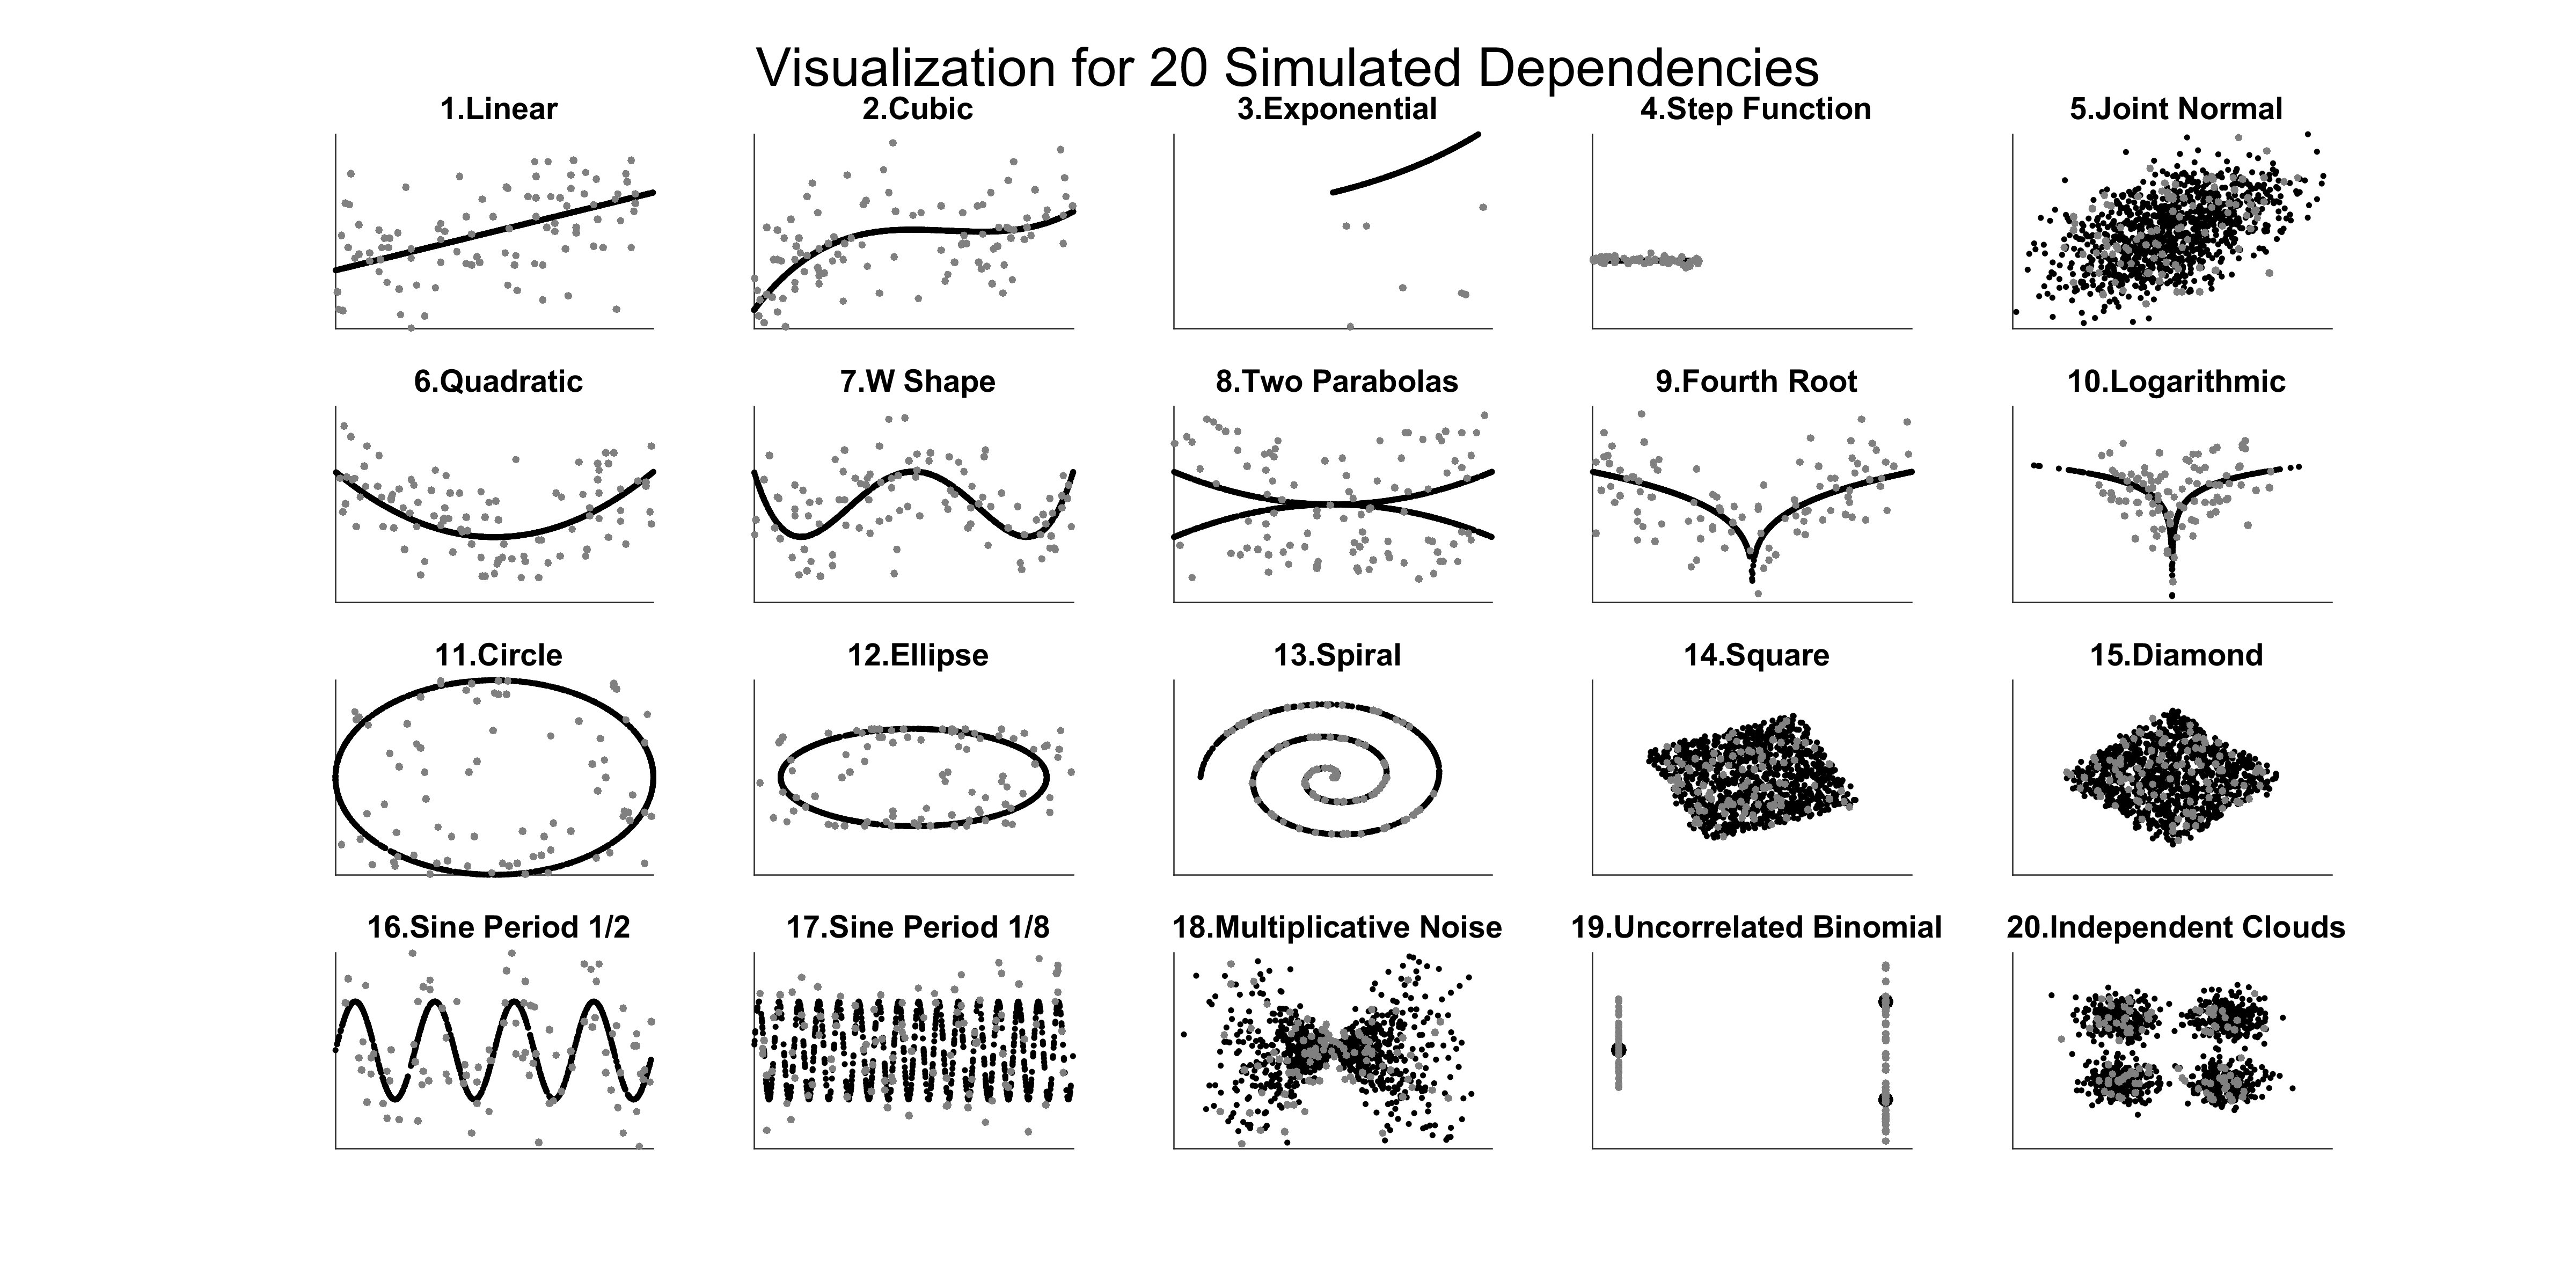
\includegraphics[trim={5cm 1.5cm 4cm 0.5cm},clip, width=1.0\textwidth]{Figures/FigSimVisual}
\caption{Visualization of the $20$ dependencies at $D=D_{y}=1$. For each, $n=100$ points are sampled with noise ($\kappa=1$) to show the actual sample data used for one-dimensional relationships (gray dots). For comparison purposes, $n=1000$ points are sampled without noise ($\kappa=0$) to highlight each underlying dependency (black dots). Note that only black points are plotted for type 19 and 20, as they do not have the noise parameter $\kappa$.
}
\label{f:dependencies}
\end{figure}

\begin{figure}[htbp]
\vspace{-50pt}
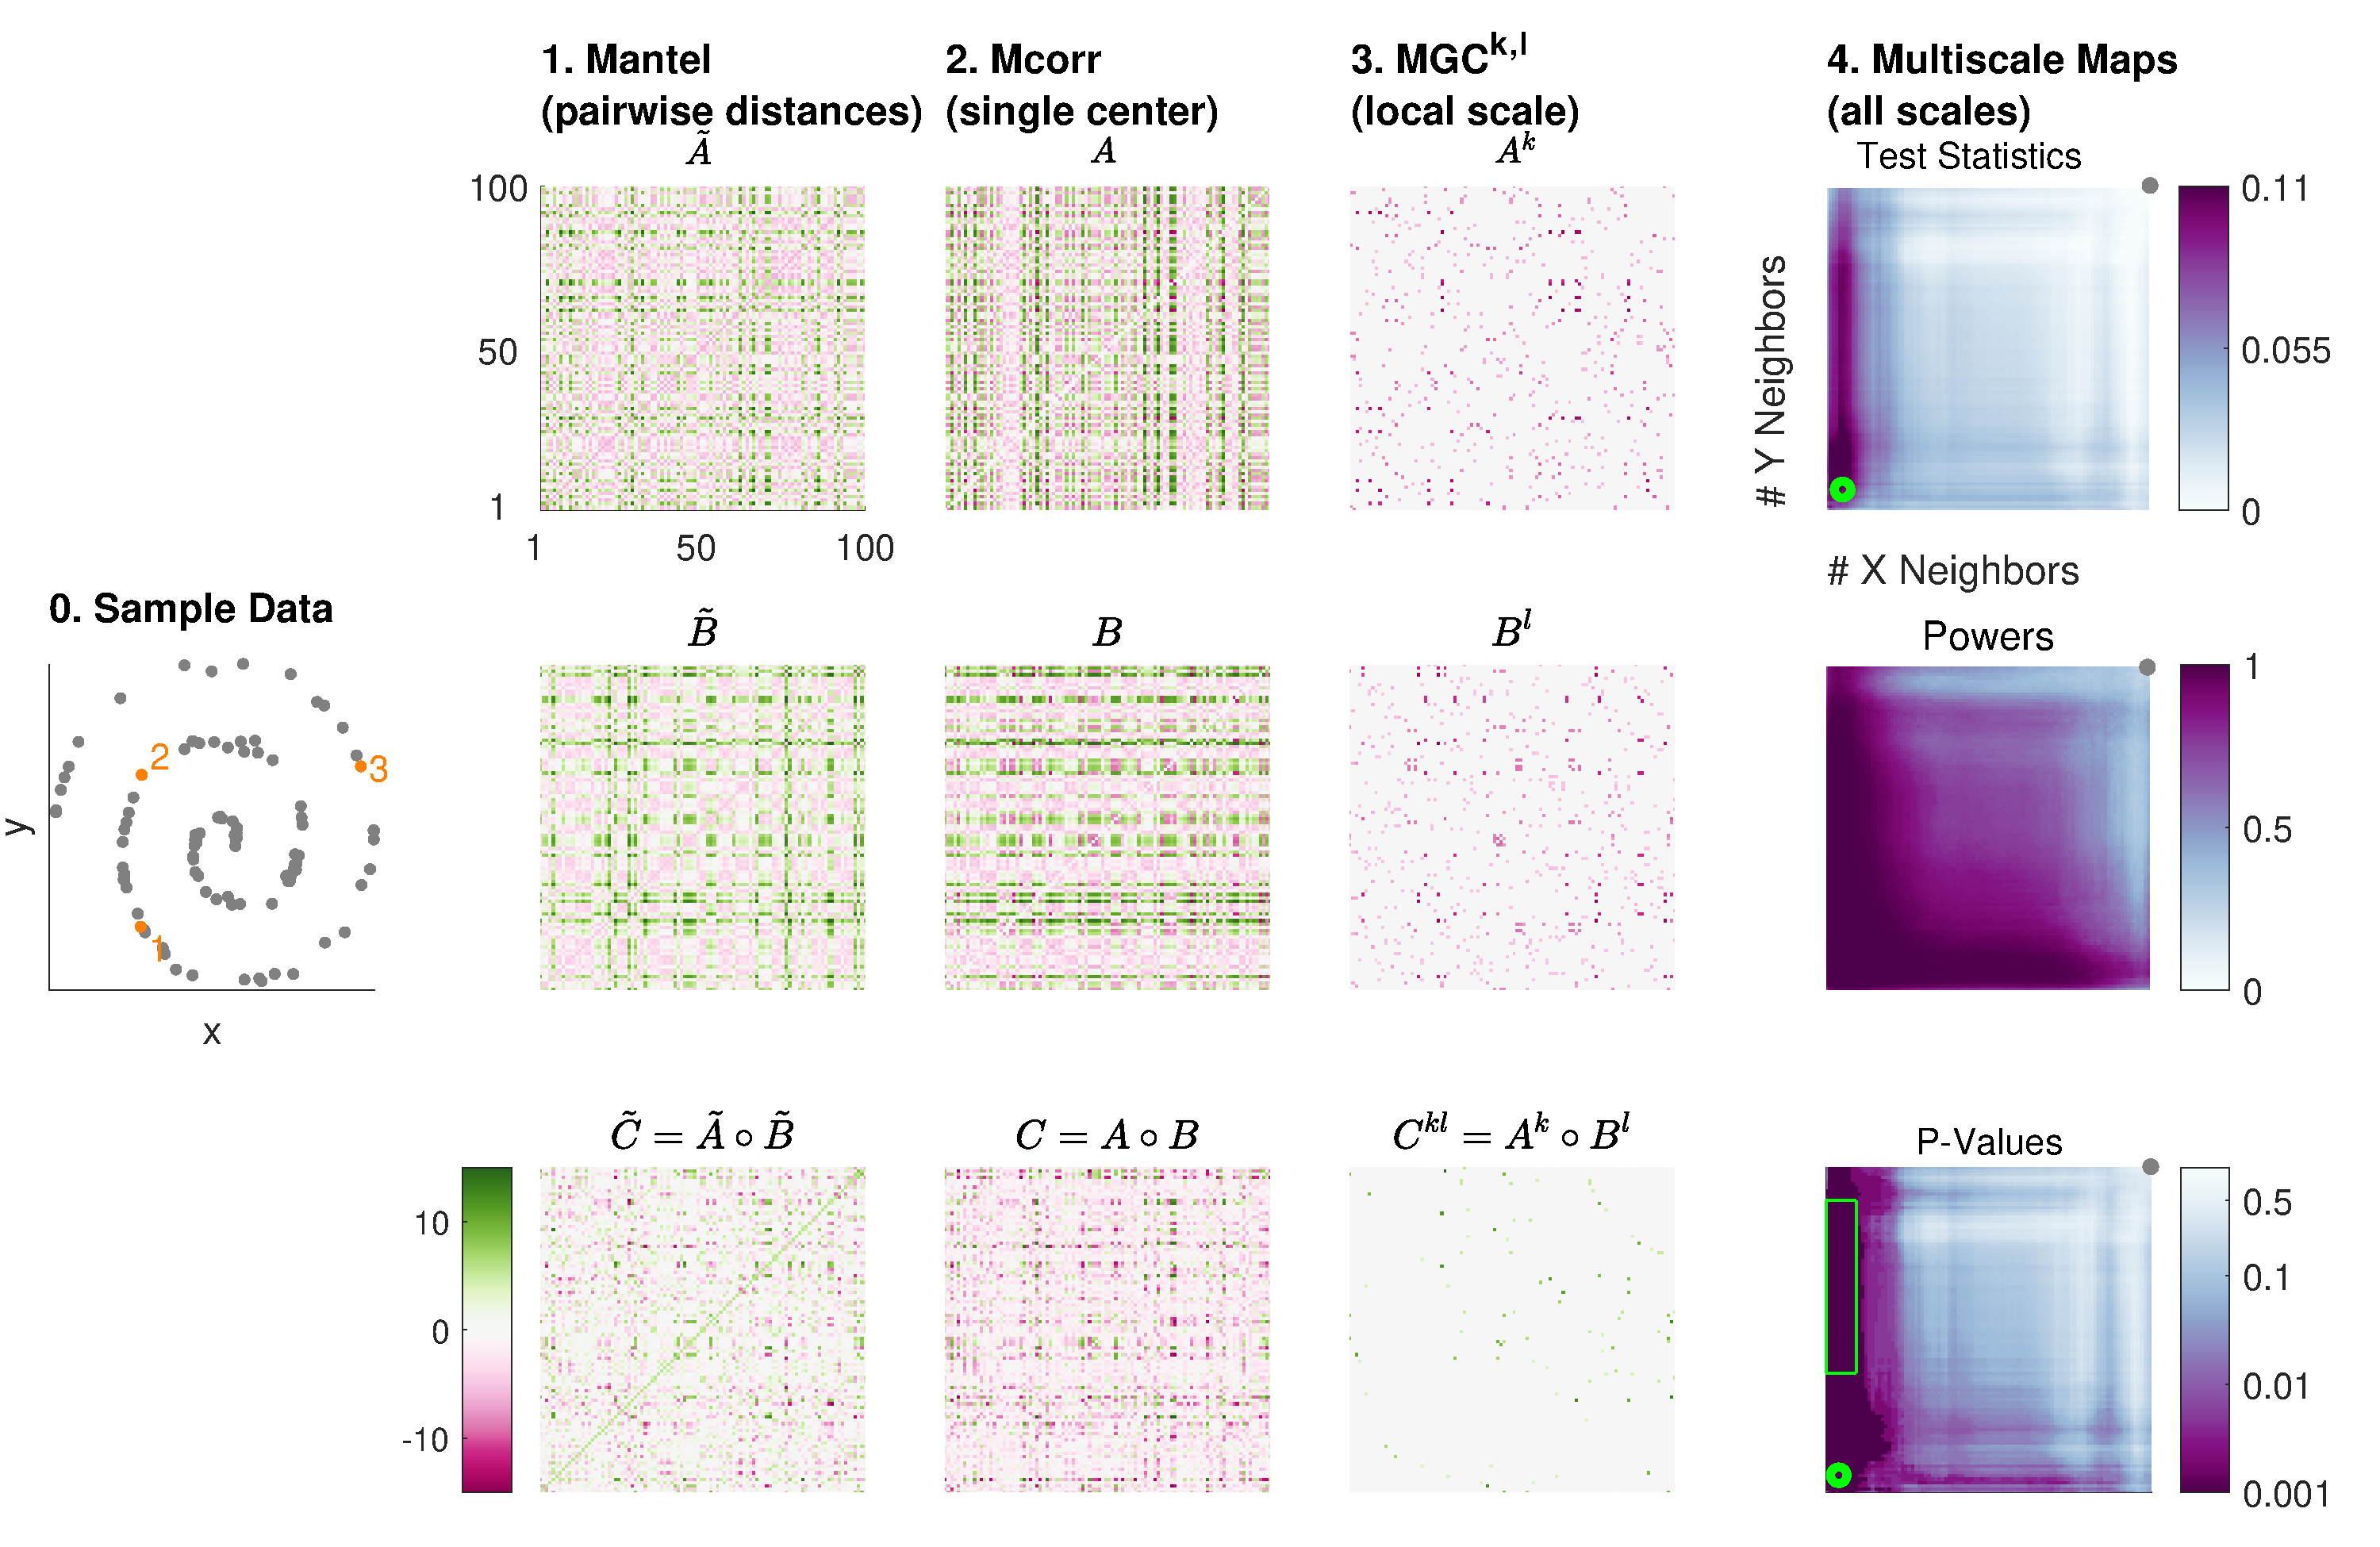
\includegraphics[width=1.0\textwidth,trim={0 0 0.75cm 0},clip]{Figures/FigA}
\setlength{\tabcolsep}{10pt} % Default value: 6pt
\begin{tabular}{r r r r}
\multicolumn{1}{l}{{\small \textbf{6. Table}}} & & & \\
$\delta_x$(1,2)   & \hspace{1.5em} \color{magenta}-2.03  & \hspace{3.5em} \color{magenta}-1.93  &  \hspace{3.0em} \color{magenta}-1.93  \\
 $\delta_y$(1,2) & \color{magenta}-2.30 & \color{magenta}-2.30 & \color{magenta}-2.30  \\
 $\delta_x \times \delta_y$ & \color{green}4.67 & \color{green}4.44 & \color{green}4.44  \\

\hline

 $\delta_x$(2,3) & \color{green}2.53 & \color{green}2.59 & 0.00  \\
 $\delta_y$(2,3) &  \color{magenta}-1.36 & \color{magenta}-2.03 & 0.00  \\
 $\delta_x \times \delta_y$ & \color{magenta}-3.43 & \color{magenta}-5.26 & 0.00  \\

\hline
 $\sum{\delta_x \times \delta_y}$ & \color{magenta}-502.61   & \color{green}92.95 & \color{green}301.33  \\
 test statistic &  \color{magenta}-0.02  & 0.00 & \color{green}0.10  \\
\end{tabular}

\begin{tikzpicture}[remember picture,overlay]
\node[xshift=-5cm,yshift=-5cm] at (current page.east){%
    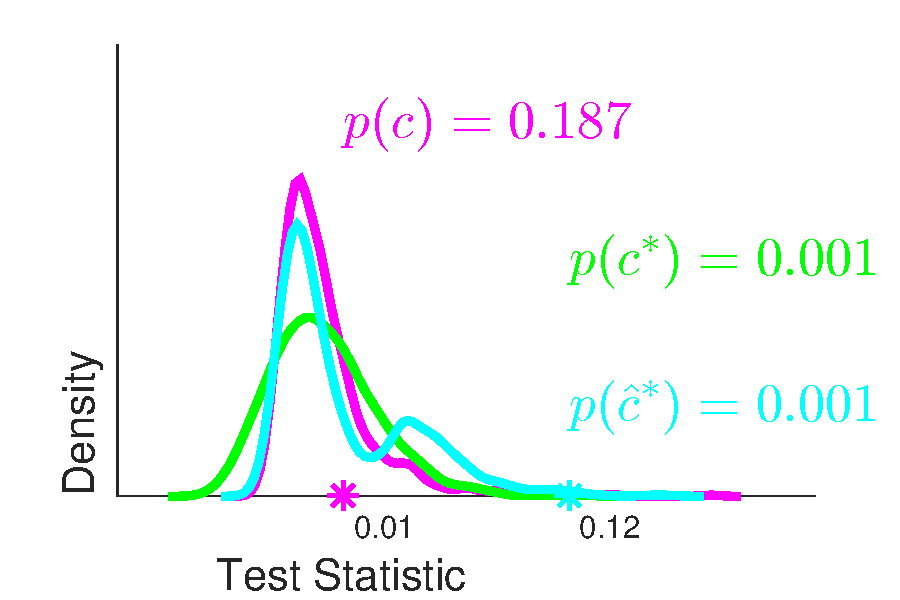
\includegraphics[width=0.35\textwidth,trim={1.5cm 0cm 1.8cm 0},clip]{Figures/FigB}};
  %\node[anchor=east,inner sep=0pt] at ($(current page.east)-(10cm,10cm)$) {
   %  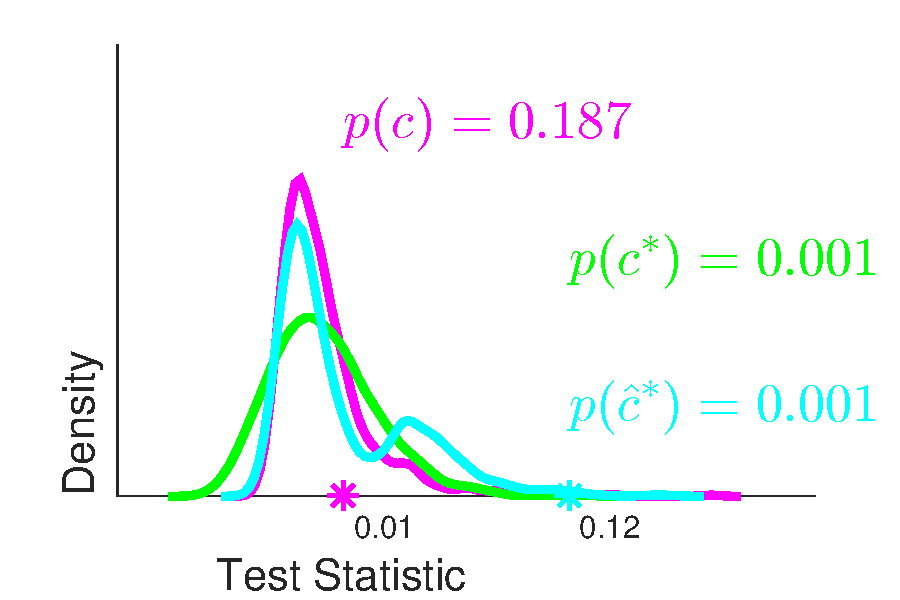
\includegraphics[width=0.3\textwidth]{Figures/FigB}
  %};
\end{tikzpicture}
\end{figure}
\clearpage
\captionof{figure}{
Schematic  and table demonstrating the ability of Multiscale Generalized Correlation (\Mgc) to detect dependence for any relationship.
\textbf{0.} 100 pairs of observations $(x_i,y_i)$ are nonlinearly (spirally) dependent on one another.
%
\textbf{1.} Choose a metric on $x$ and another on $y$, and compute all pairwise distances (centered by the overall means) for $x$ and $y$ yielding interpoint comparison matrices
 $\tilde{A}$ (top) and $\tilde{B}$ (middle),
and their joint distance matrix $\tilde{C}=\tilde{A} \circ \tilde{B}$ (bottom), whose normalized sum is the  \Mantel~statistic \cite{Mantel1967} (bottom row of table).
%
\textbf{2.} Single centering --- subtract the row-sums from $\tilde{A}$ and column-sums from $\tilde{B}$ to eliminate bias due to individual samples --- yields $A=\{a_{ij}\}$ and $B=\{b_{ij}\}$; the normalized sum of their  element-wise product  $C$ is equivalent to the  \Mcorr~statistic \cite{SzekelyRizzo2013a}.
%
\textbf{3.} Given a local scale, for example, $k=l=4$ here, yields $A^{k}$, $B^{l}$, and $C^{kl}$.  All these test statistics are normalized sums of the element-wise products. The fact that \Mgc~yields a $C^{kl}$ matrix that is all positive (green), whereas the others yield $C$ matrices with both positive and negative values (purple), suggest that \Mgc~will correctly report a large test statistic here, resulting in a small p-value.
\textbf{4.} Compute the test statistic (top), power (middle), and p-value (bottom) for all local scales, resulting in multiscale maps that reveal the scales of dependency. Green dots show the scale of estimated test statistic by Sample \Mgc, and the green box shows the estimated optimal scales.
\textbf{5.} Report the corresponding observed test statistics and p-values, and discover the optimal scales (green rectangle in  significance map) using Sample \Mgc.
Whereas \Mcorr, the global test, has very low power (gray dot in  significance map)
and therefore yields a small statistic and a non-significant p-value ($0.257$),  there are many local scales that achieve nearly perfect power, so both Oracle (green line) and Sample (cyan line) \Mgc~($\GG^{*}$ and $\hat{\GG}^{*}$) obtain large test statistics and highly significant p-values ($\approx 0.001$) and reveal the scales of dependency.
\textbf{6.} Numerical demonstration of how \Mgc~is able to detect dependence even in highly nonlinear and low-sample size settings. The three colored points in the scatter plot indicate the three points considered in this table.
The global methods fail to detect significant dependence since they consider all pairs, including the non-local ones, which \emph{negatively} impact the degree of dependence estimated.
\Mgc~only considers pairs that are jointly local (such as $(1,2)$), while discarding other pairs (such as $(2,3)$).
}
\label{f:schematic}


\begin{figure}[htbp]
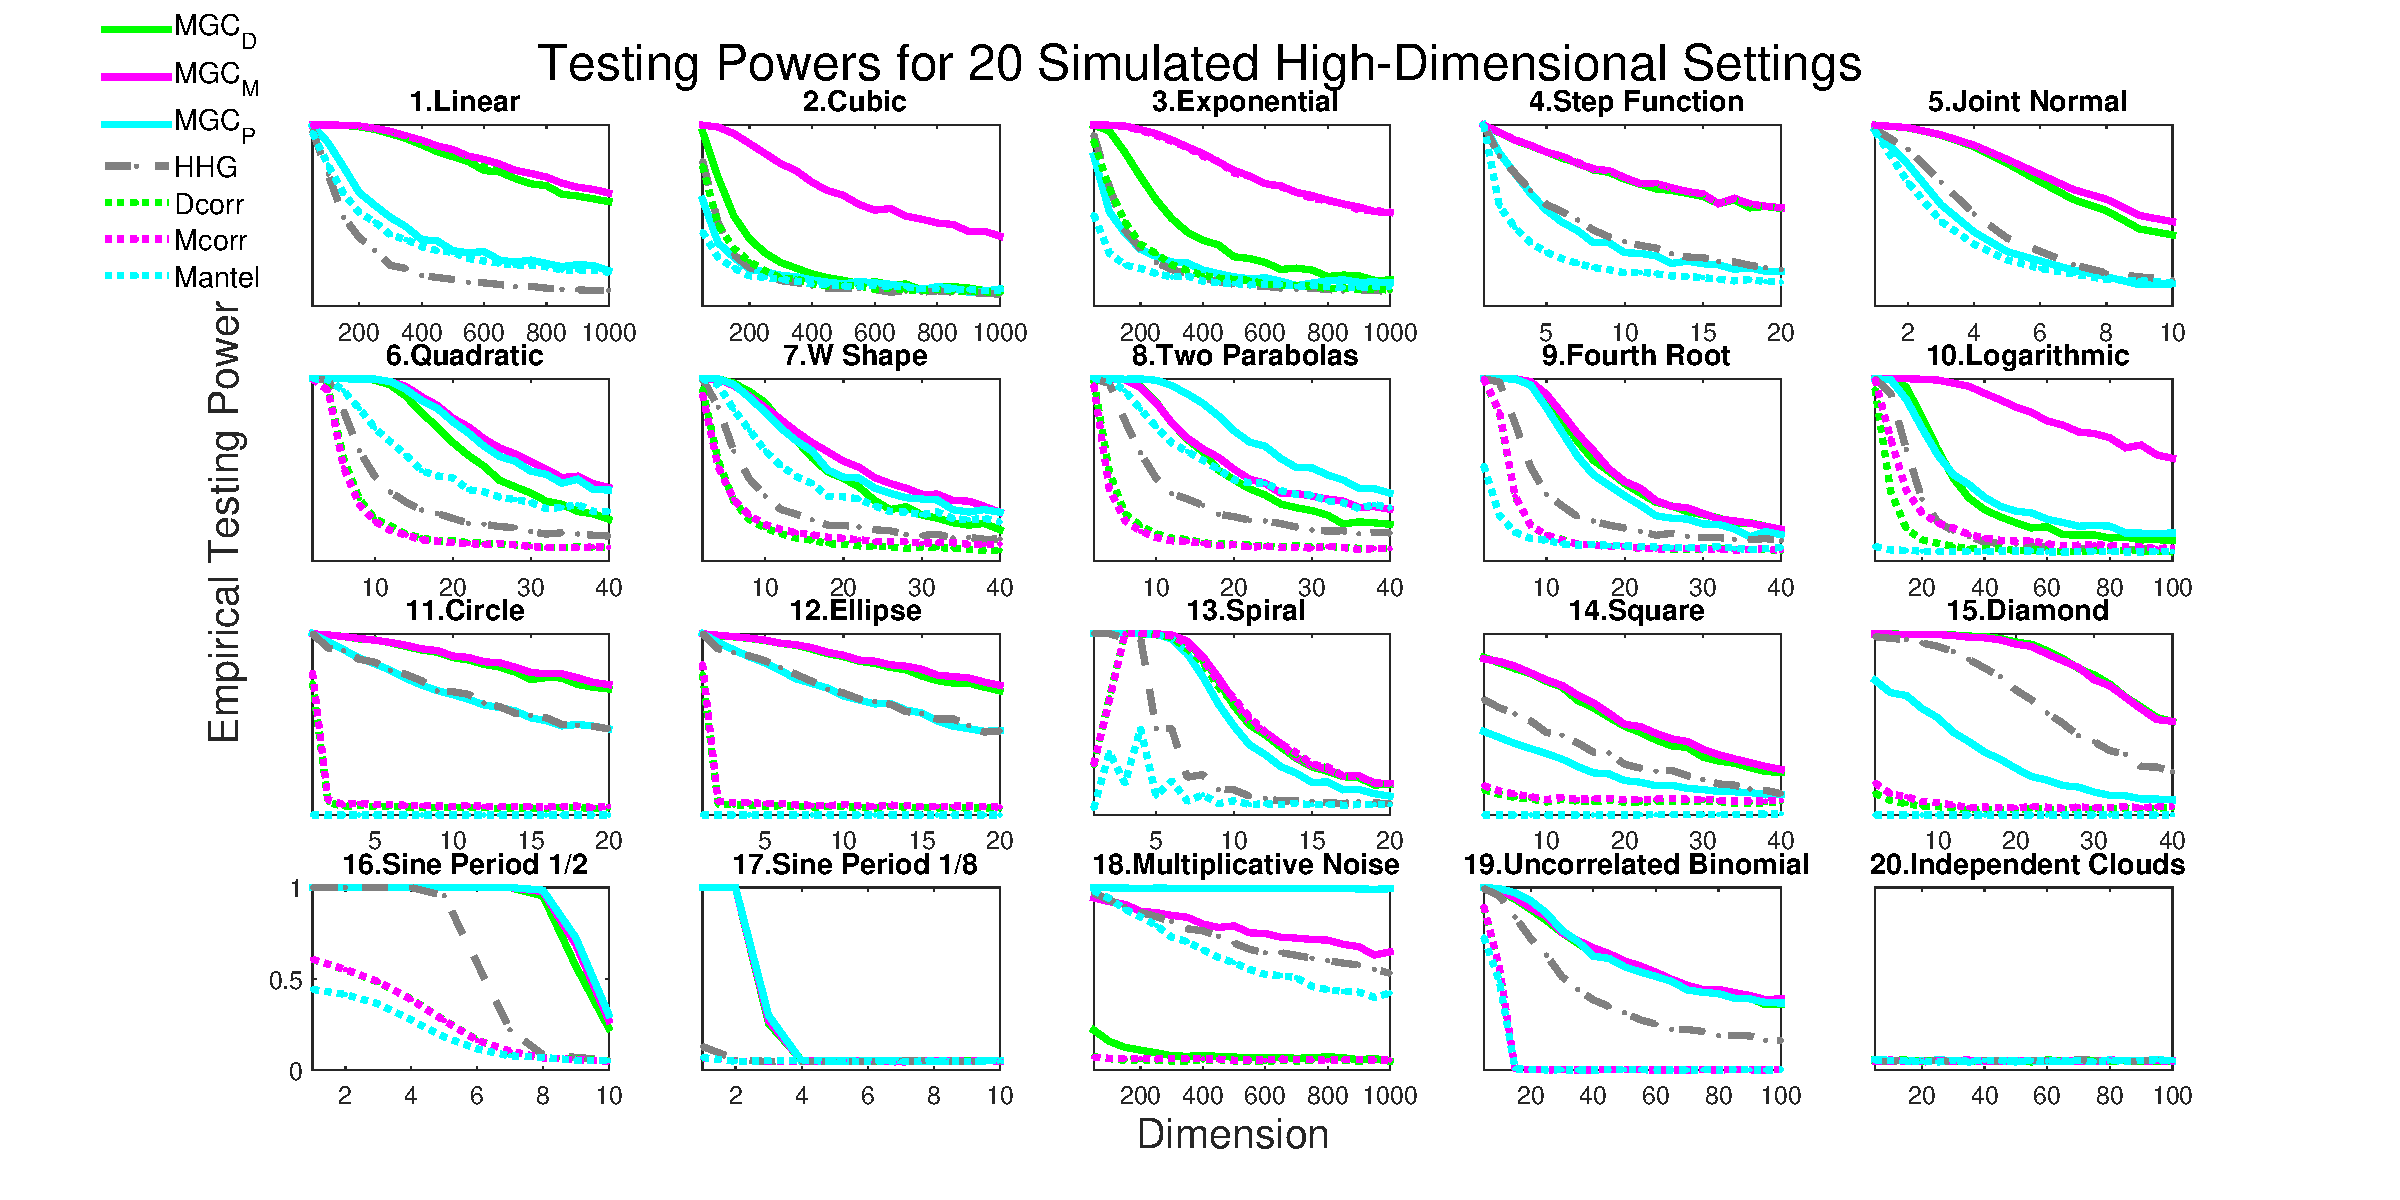
\includegraphics[width=1.0\textwidth,trim={0 0.5cm 3.2cm 0},clip]{Figures/FigHDPowerAll}
\caption{Power of different methods for $20$ different dependence relationships, estimated by Monte Carlo independence tests (see Algorithm \ref{alg:power} for details). It includes eight different tests: \Mcorr, \Dcorr, and \Mantel~(gray solid, dashed, and dashdot lines, respectively), their corresponding Oracle \Mgc~counterparts, \Mgcm, \Mgcd, \Mgcp~(green with same line styles), Sample \Mgc~applied to \Mcorr~(cyan solid), and \Hhg~(gray dotted line).
Each panel shows the testing power at significance level $\alpha=0.05$ versus the dimensionality of $\mb{x}$'s, for $n=100$ samples.
Excluding the independent relationship (\#20), for which all methods yield power $0.05$, as they should, Oracle \Mgc~empirically achieves similar or better power than its respective global counterpart. Moreover, Sample \Mgc~is very close to Oracle \Mgcm, and overall dominates existing approaches for almost all relationships and all dimensions, including \Hhg~\cite{HellerGorfine2013}, another state-of-the-art method. Note that \Mgc~is always plotted ``on top'' of the global variants if there is overlap, therefore, some of the global variants are not always visible from the display.}
\label{f:nDAll}
\end{figure}

\begin{figure}[htbp]
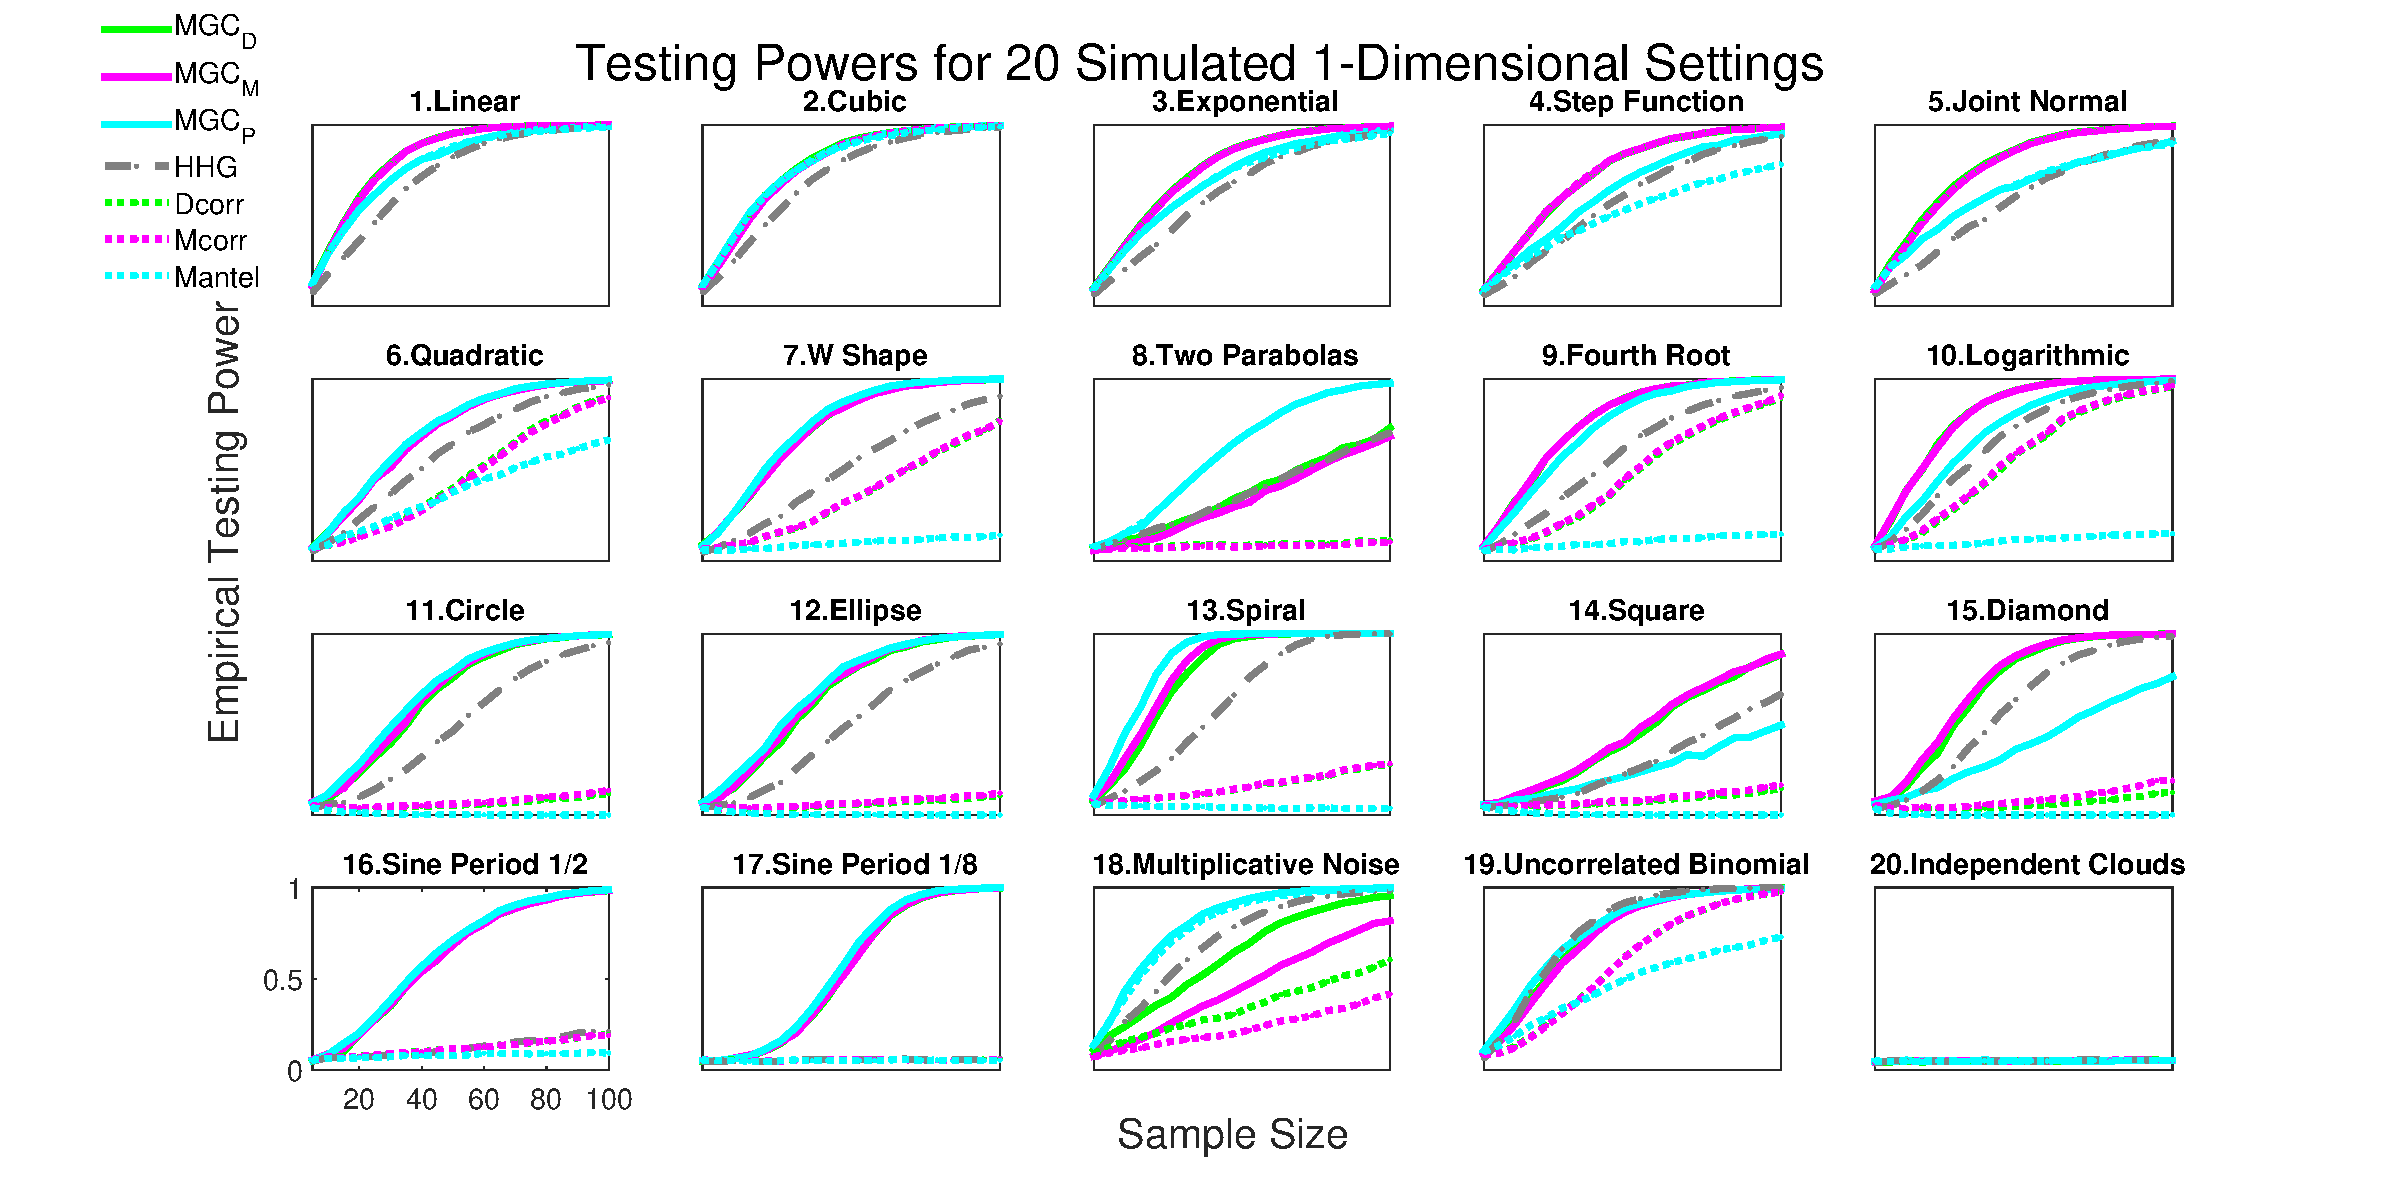
\includegraphics[width=1.0\textwidth,trim={0 0.5cm 3.2cm 0},clip]{Figures/Fig1DPowerAll}
\caption{
The same power plots as in Figure~\ref{f:nDAll}, except the $20$ dependence relationships are one-dimensional with noise, and the x-axis shows sample size increasing from $5$ to $100$.
Again, Oracle \Mgc~empirically achieves similar or better power than the previous state-of-the-art approaches for all sample sizes on almost all problems, with Sample \Mgc~being very close to Oracle \Mgc~and overall superior to other benchmarks for essentially all dependency structures and sample sizes.}
\label{f:1DAll}
\end{figure}

\begin{figure}[!ht]
\centering
% \subfigure{
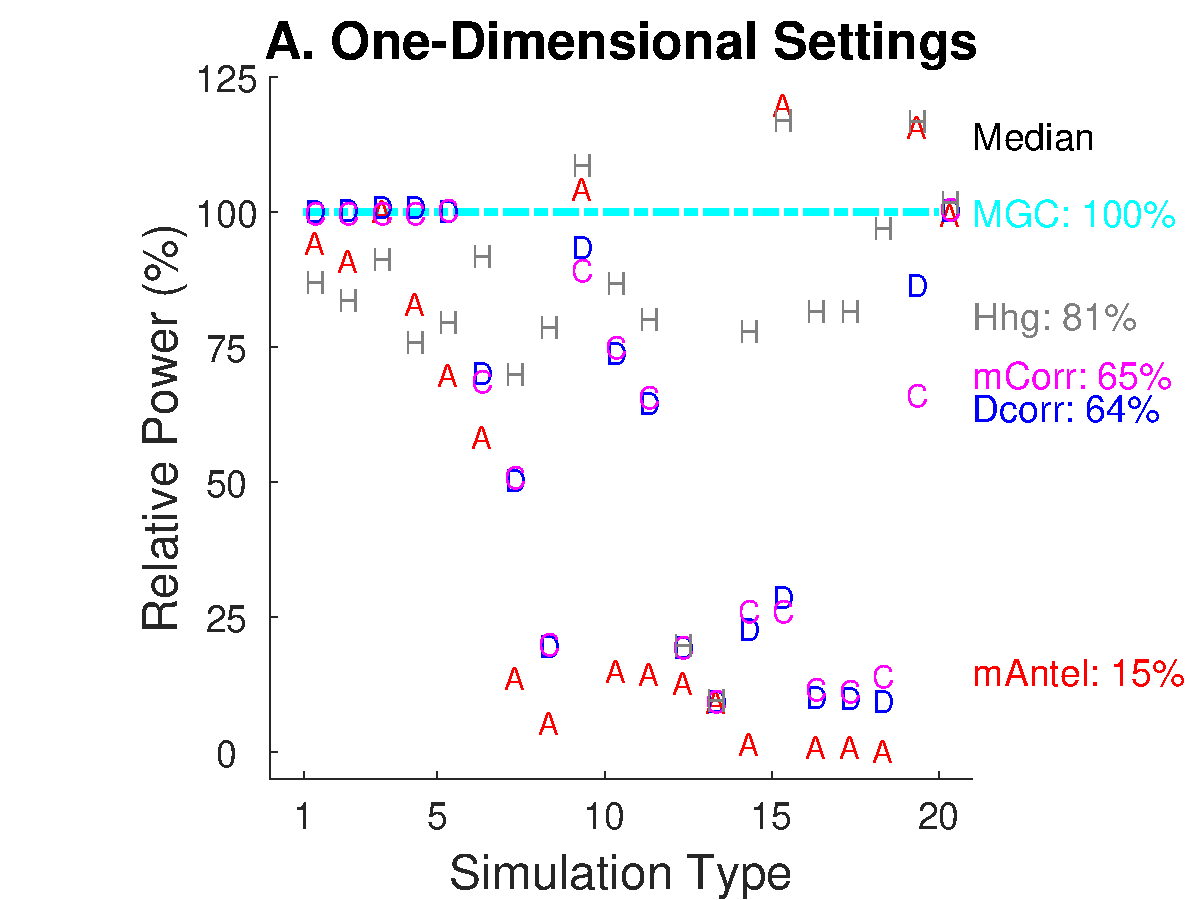
\includegraphics[width=0.48\textwidth,trim={1.5cm 0 0cm 0cm},clip]{Figures/Fig1DPowerSummary}
% }
% \subfigure{
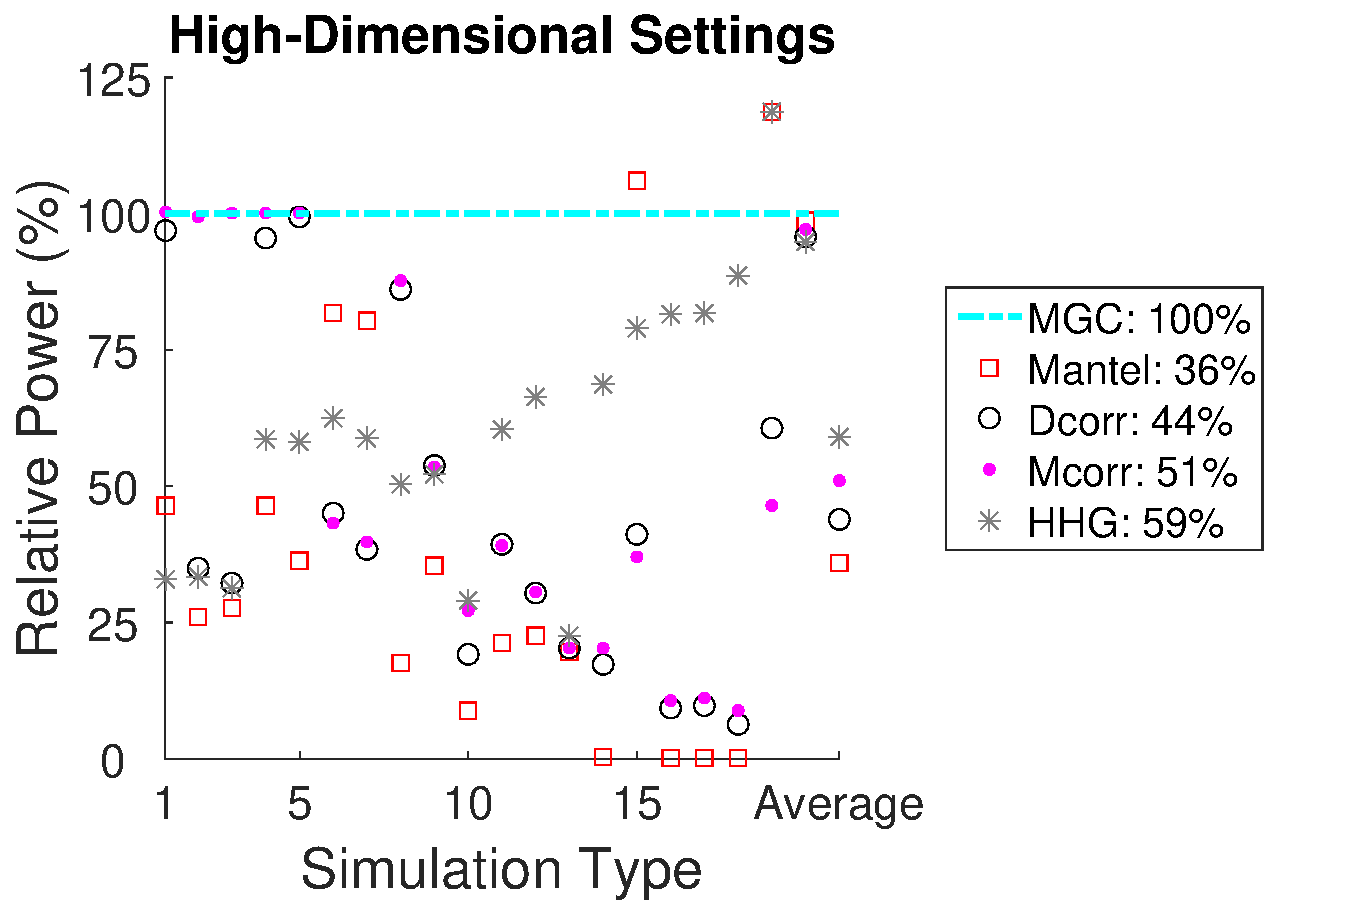
\includegraphics[width=0.48\textwidth,trim={1.5cm 0 0cm 0cm},clip]{Figures/FigHDPowerSummary}
% }
  \caption{Relative Power of  \Mgc~to four benchmark dependence tests, for the $20$ different relationships under high-dimensional and one-dimensional relationships.
Let $\bar{\beta}_s(\mathcal{A})$ denote the average power for a given problem setting $s$ and algorithm $\mc{A}$ in Figure~\ref{f:nDAll} and ~\ref{f:1DAll}, which averages over the sample size in case of the one-dimensional scenario and averages over the dimensional choice in case of the high-dimensional scenario. The x-axis is the simulation type, and y-axis shows the relative power of existing competitors to \Mgc~via $\bar{\beta}_s(\mathcal{A}) / \bar{\beta}_s(\Mgc)$. The last column shows the median relative power throughout all simulation types (excluding the independent relationship of type $20$). The percentages indicate that \Mgc~nearly dominates all benchmarks, exhibiting similar or better power for nearly all settings.
}
\label{f:Summary2}
\end{figure}


\begin{figure}[htbp]
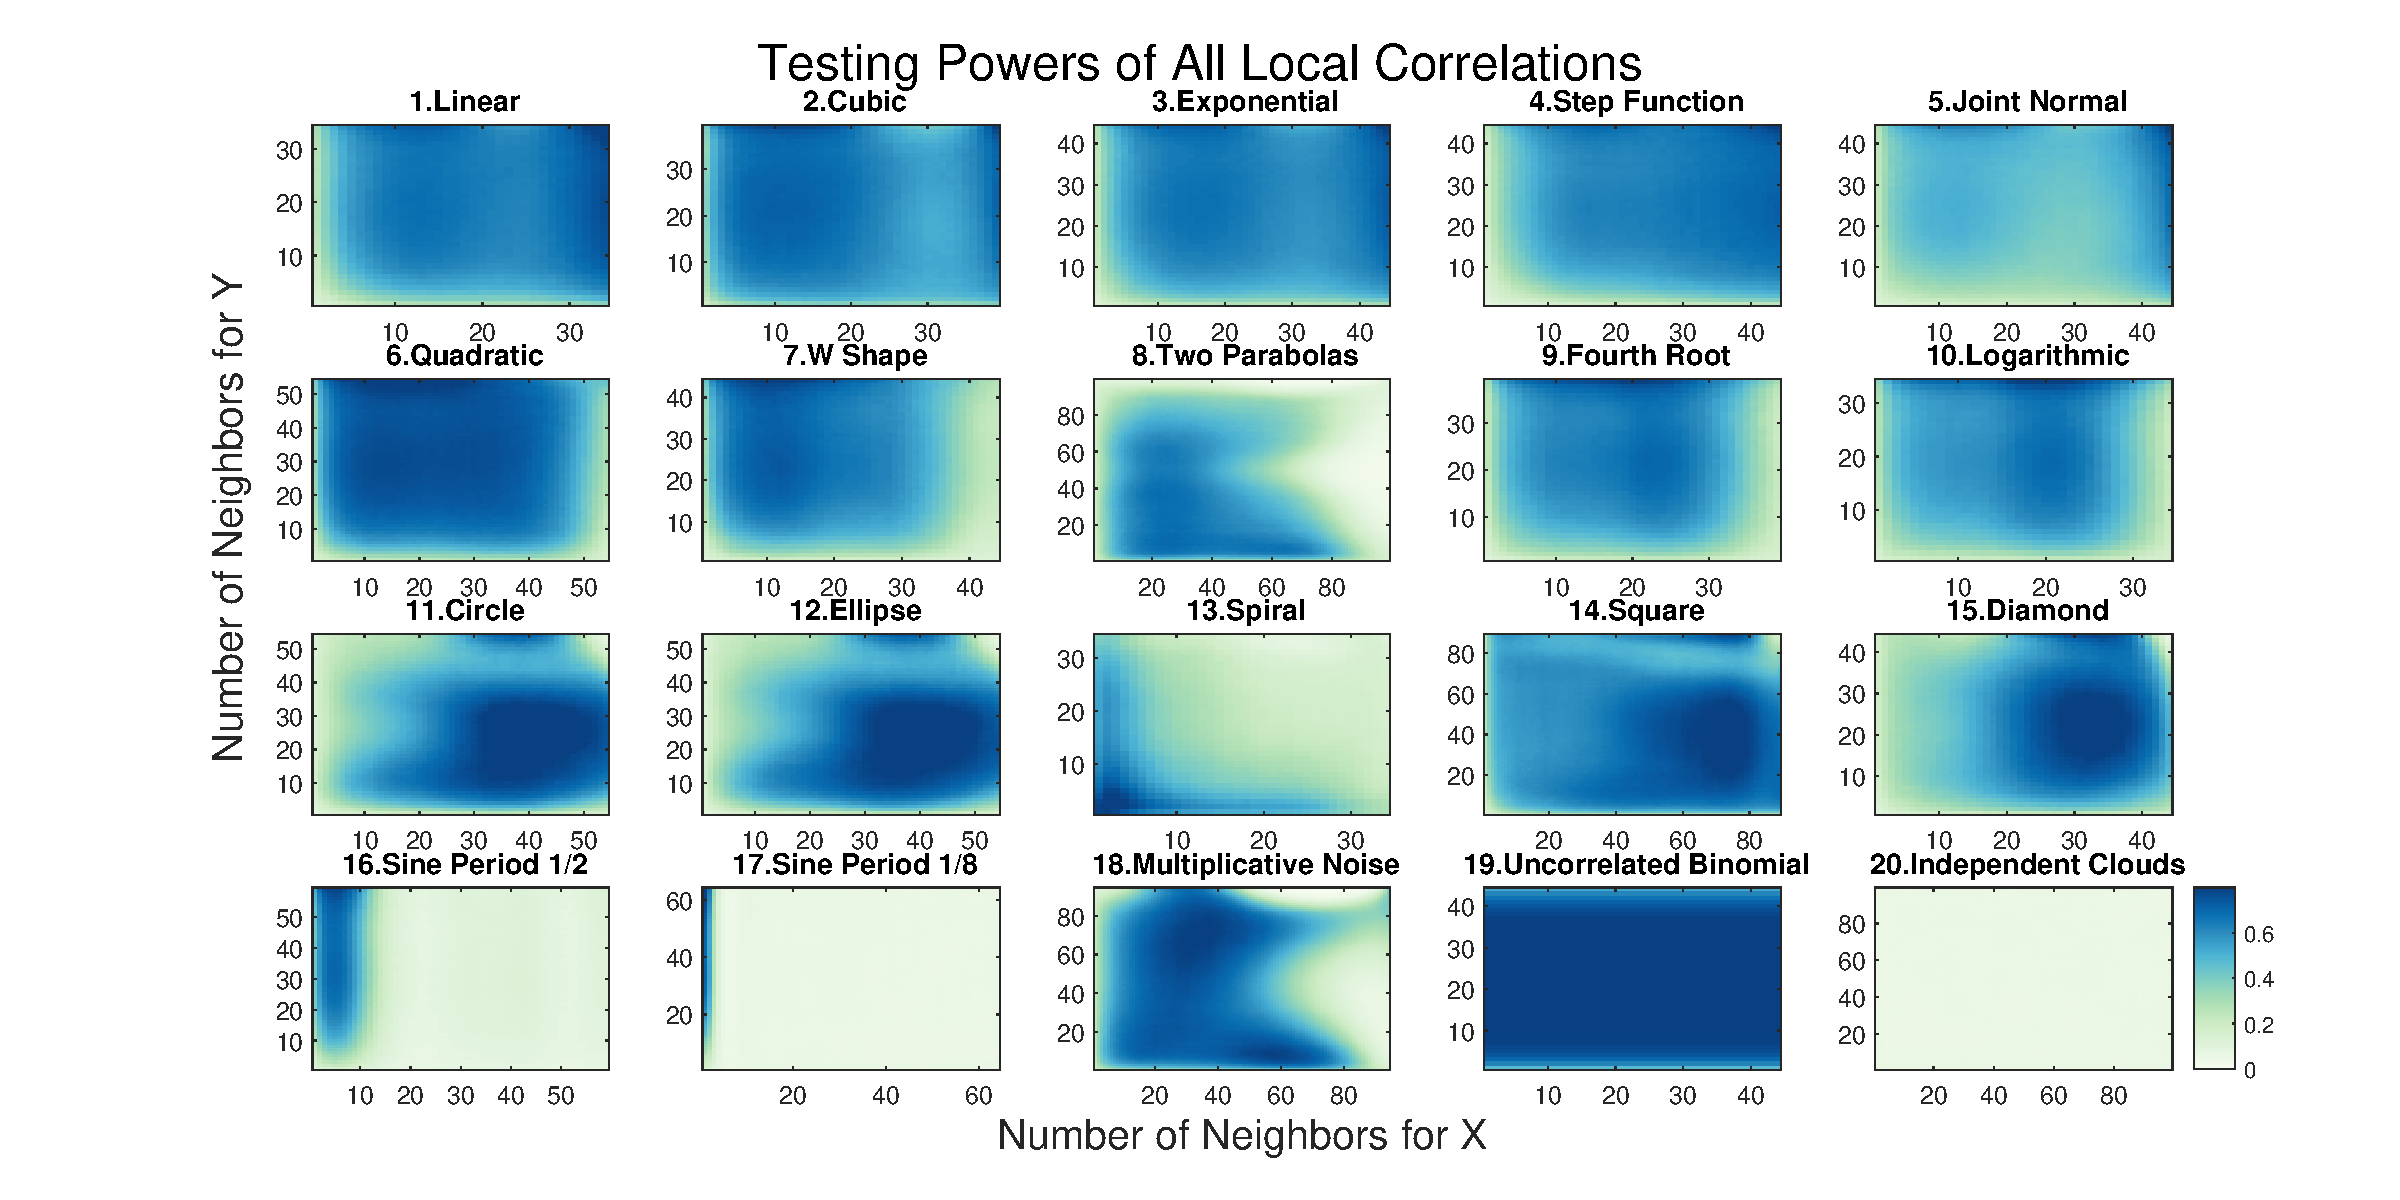
\includegraphics[width=1.0\textwidth,trim={3cm 0.5cm 1.8cm 0.5cm},clip]{Figures/Fig1DHeat}
\caption{Multiscale Power Maps indicating the influence of neighborhood size on \Mgc~testing power, for the one-dimensional simulations in Figure~\ref{f:1DAll}. For each simulation,  the sample size is $n=60$, and the significance level is $\alpha=0.05$. It has similar behavior and interpretation as the high-dimensional power maps in Figure~\ref{f:powermaps}.}
\label{f:powermaps1}
\end{figure}

\clearpage
\section{Real Data Processing}
\label{appen:real}

\subsection{Brain Activity vs Personality}
\label{app:personality}

This experiment investigates whether there is any dependency between resting brain activity and personality. Human personality has been intensively studied for many decades; the most widely used and studied approach is the NEO Personality Inventory-Revised the characterized personality along five dimensions \cite{Costa1992}.
%
This dataset consists of $42$ subjects, each with  $197$ time-steps of resting-state functional magnetic resonance activity (rs-fMRI) activity, as well as the subject's five-dimensional ``personality''. Adelstein et al. \cite{AdelsteinEtAl2011} were able to detect dependence between the activity of certain brain regions and dimensions of personality, but lacked the tools to test for dependence of whole brain activity against all five dimensions of personality.
%
For the five-factor personality modality, we  used the Euclidean distance. For the brain activity modality,
we derived the following comparison function. For each scan, (i) run Configurable Pipeline for the
 Analysis of Connectomes pipeline \cite{CPAC2015} to process the raw brain images yielding a parcellation into
197 regions of interest,
(ii) run a spectral analysis on each region and keep the power of band,
(iii) bandpass and normalize it to sum to one,
(iv) calculate the Kullback-Leibler divergence across regions to obtain a similarity matrix across comparing all regions.
Then, use the normalized Hellinger distance to compute distances between each subject.


\subsection{Brain Connectivity vs Creativity}
\label{app:creativity}

This experiment investigates whether there is any dependency between brain structural networks and creativity. Creativity has  been extensively studied in  psychology; the ``creativity composite index'' (CCI) is an index similar to an ``intelligence quotient'' but for creativity rather than intelligence \cite{Jung2009}.
%
This dataset consists of $109$ subjects, each with diffusion weighted MRI data as well as the subject's CCI.
Neural correlates of CCI have previously been investigated, though largely using structural MRI and cortical thickness \cite{Jung2009}.  Previously published results explored the relationship between graphs and  CCI \cite{Koutra15a}, but did not provide a valid test.
%
We used Euclidean distance to compare CCI values.
For the raw brain imaging data, we derived the following comparison function.  For each scan we estimated brain networks from diffusion and structural MRI data via  \Migraine, a pipeline for estimating brain networks from diffusion data \cite{GrayRoncal2013}.
We compute the distance between the graphs using the semi-parametric graph test statistic \cite{Sussman2013,ShenVogelsteinPriebe2016,Tang2016}, embedding each graph into two dimensions and aligning the embeddings via a Procrustes analysis.

\subsection{Brain Shape vs Depression}
\label{app:depression}

This experiment investigates whether there is any dependency between brain shape and depression.
This  dataset consists of $114$ subjects. Each subject has a structural MRI scan as well as a discrete variable indicating whether the subject is non-affected, high-risk, or clinically depressed.
Previous investigations have linked major depressive disorder to hippocampus shape \cite{ParkEtAl2008,PosenerEtAl2003}, though global tests were unable to detect a statistically significant dependence structure at the $\alpha=0.05$ level.
% From the MRI data, previous work extracted both the left and right hippocampi.
For the brain shape modality, we computed the distance utilizing  nonlinear landmark matching approach called Large Deformation Diffeomorphic Metric Mapping
 \cite{ParkEtAl2008,BegEtAl2005}.
For the depression variable, we used the Euclidean distance.



\subsection{Proteins vs Cancer}
\label{app:cancer}
%  method establishment and data analysis

This experiment investigated whether there is any dependency between abundance levels of peptides in human plasma and the presence of cancers.  Selected Reaction Monitoring (SRM) is a targeted quantitative proteomics technique for measuring protein and peptide abundance in complicated biological samples \cite{PMID21248225}. In a previous study, we used SRM to identify $318$ peptides from
$33$ normal, $12$ pancreatic cancer, $29$ colorectal cancer, and $24$ ovarian cancer samples \cite{Wang2017}. Then, using other methods, we identifed three peptides that were implicated in ovarian cancer, and validated them as legitimate biomarkers with a follow-up experiment.
%
% SRM transition parameters (precursor ion M/z, fragmented ion M/z, collision energy, and dwell time) were optimized through using synthetic peptides. 200 $\mu$l human plasma from each individual (healthy or cancer patient) were depleted to remove top 14 high abundance proteins using a Seppro IgY14 LC10 column system purchased from Sigma-Aldrich (St. Louis, Missouri). Depleted human plasma samples were denatured, reduced, alkylated, trypsin-digested, and cleaned through hydrophobic solid phase extraction methods as previously described \cite{PMID21248225, Wang2017}. Target peptide abundances in each sample were determined using a set of SRM methods established using synthetic target peptides. The abundance of a target peptide was represented by the total area under the curve (AUC) of all its SRM transitions normalized to the total AUC of all SRM transitions from a heavy isotope labeled internal control peptide spiked with the same amount (3 femtomole) before the assay.
% Normalized AUC values for all the peptides in each sample were calculated to represent the relative abundances of the target peptides.
% %
% $33$ normal, $12$ pancreatic cancer, $29$ colorectal cancer, and $24$ ovarian cancer plasma samples were analyzed for the abundances of a panel of $318$ peptides. %, so the protein data is of size $318 \times 98$.

In this study, we performed the following five sets of tests on those data:
\begin{compactenum}
\item  ovarian vs.~normal for all proteins,
\item ovarian vs.~normal for each individual protein,
\item  pancreas vs.~normal for all proteins,
\item  pancreas vs.~all others for each individual protein,
\item pancreas vs.~normal for each individual protein.
\end{compactenum}
%
These tests are designed to first validate the \Mgc~method from ovarian cancer, then identify biomarkers unique to pancreatic cancer, that is, find a protein that is able to tell the difference between pancreas and normals, as well as pancreas vs all other cancers.
%
For each of the five tests, we create a binary label vector, with $1$ indicating the cancer type of interest for the corresponding subject, and $0$ otherwise. Then each algorithm is applied to each task.
For all tests we used Euclidean distances and the type $1$ error level is set to $\alpha=0.05$
The three test sets assessing individual proteins provide $318$ p-values; we used
% For the first two tests, the Euclidean distance of the peptides data is based on all proteins; for the last three screening tasks, the Euclidean distance matrix is based on each peptide, such that $318$ tests and p-values are reported. The type $1$ error level is set to $\alpha=0.05$, with
the Benjamini-Hochberg procedure \cite{Benjamini1995}  to control the false discovery rate. A summary of the results are reported in Table~\ref{t:real2}.



% For the first two tests, \Mgc~reports as low or lower p-value than others.
% %
% % For the, and is the only method other than \Hhg~that can reveal useful proteins for pancreas versus normal persons and also pancreas versus all other cancer types.
% %
% For the third test, i.e., feature screening for ovarian vs. normal, previously we validated three peptides by other techniques: peptidyl-prolyl cis-trans isomerase A, dynamin-3 isoform b, peptidyl-prolyl cis-trans isomerase A. It turns out that all three peptides have p-value $0$ for all methods including \Mgc, that is, they are all correctly identified as significant. However, there are a large number of significant peptides identified for each method as shown in Table~\ref{t:real2} third column. By ranking the peptides based on the actual test statistic of each peptide, the three peptides have rank $9,118,44$ by \Mgc, $143,92,33$ by \Mantel, $178,95,36$ by \Dcorr~and \Mcorr, $88,111,12$ by \Hhg. \Mgc~is the method that rank the three known biomarkers the best.
%
% For the last two tests exploring pancreatic, both \Mgc~and \Hhg~reveal the same unique protein for pancreas: neurogranin. \Hhg~also identifies another peptide (tropomyosin alpha-3 chain isoform 4). However, tropomyosin is a ubiquitously expressed protein, since normal tissues and other cancers will also express tropomyosin and leak it into blood, whereas neurogranin is exclusively expressed only in brain tissues. Moreover, there exists strong evidence of tropomyosin 3 upregulated in other cancers \cite{TPM1,TPM2,TPM3,TPM4}. Therefore, initial literature search suggests that tropomyosin is likely falsely identified by \Hhg~and less useful for pancreas, whereas neurogranin is a more promising protein for follow-ups that is uniquely identified by \Mgc.


\begin{table*}[!ht]
\centering
\caption{Results for cancer peptide screening. The first two rows report the p-values for the tests of interest based on all peptides. The next four rows report the number of significant proteins from individual peptide tests; the Benjamini-Hochberg procedure is used to locate the significant peptides by controlling the false discovery rate at $0.05$.}
\label{t:real2}%
\begin{tabular}{|l|l||c|c|c|c|c|}
\hline
& Testing Pairs / Methods & Sample \Mgc & \Mantel & \Dcorr & \Mcorr & \Hhg \\
\hline
1 & Ovar vs. Norm: p-value & $\textbf{0.0001}$  & $\textbf{0.0001}$ & $\textbf{0.0001}$ & $\textbf{0.0001}$ & $\textbf{0.0001}$ \\
\hline
2 & Ovar vs. Norm: \# peptides  & $218$  & $190$ & $186$ & $178$ & $225$ \\
\hline \hline
3 & Pancr vs. Norm: p-value & $\mathbf{0.0082}$  & ${0.0685}$ & $0.0669$ & $0.0192$ & ${0.0328}$ \\
\hline
4 & Panc vs. Norm: \# peptides & $9$  & $7$ & $6$ & $7$ & $11$ \\
\hline
5 & Panc vs. All: \# peptides & $1$  & $0$ & $0$ & $0$ & $3$ \\
\hline
6 & \# peptides unique to Panc & $1$  & $0$ & $0$ & $0$ & $2$ \\
\hline
7 & \# false positives for Panc & $\mathbf{0}$  & n/a & n/a & n/a & $1$ \\
\hline
\end{tabular}
\end{table*}

All methods are able to successfully detect a dependence between peptide abundances in ovarian cancer samples versus normal samples (Table \ref{t:real2}, line 1). This is likely because there are so many individual peptides that have different abundance distributions between ovarian and normal samples (Table \ref{t:real2}, line 2).  Nonetheless, \Mgc~identified more putative biomarkers than any of the other methods.  While we have not checked all of them with subsequent experiments to identify potential false positives, we do know from previous experiments that three peptides in particular are effective biomarkers.
%
% For the first two tests, \Mgc~reports as low or lower p-value than others.
%
% For the, and is the only method other than \Hhg~that can reveal useful proteins for pancreas versus normal persons and also pancreas versus all other cancer types.
%
% For the third test, i.e., feature screening for ovarian vs. normal, previously we validated three peptides by other techniques: peptidyl-prolyl cis-trans isomerase A, dynamin-3 isoform b, peptidyl-prolyl cis-trans isomerase A.
% It turns out that
All three peptides have p-value $\approx 0$ for all methods including \Mgc, that is, they are all correctly identified as significant.
% However, there are a large number of significant peptides identified for each method as shown in Table~\ref{t:real2} third column.
However, by ranking the peptides based on the actual test statistic of each peptide,
% the three peptides have rank $101,69,15$ by \Mgc, $143,92,33$ by \Mantel, $178,95,36$ by \Dcorr~and \Mcorr, $88,111,12$ by \Hhg.
\Mgc~is the method that ranks the three known biomarkers the lowest, suggesting that it is the least likely to falsely identify peptides.

We then investigated the pancreatic samples in an effort to identify biomarkers that are unique to pancreas. We first checked whether the methods could identify a difference using all the peptides.  Indeed, three of the five methods found a dependence at the $0.05$ level, with Sample \Mgc~obtaining the lowest p-value (Table \ref{t:real2}, line 3).  We then investigated how many individual peptides the methods identified; all of them found 6 to 11 peptides with a significant difference between pancreatic and normal samples (Table \ref{t:real2}, line 4).  Because we were interested in identifying peptides that were uniquely useful for pancreatic cancer, we then compared pancreatic samples to all others.  Only \Mgc~and \Hhg~identified any peptides that expressed different abundances in this more challenging case (Table \ref{t:real2}, line 5).  To identify peptides that are unique to pancreatic cancer, we looked at the set of peptides that were both different from normals and different from all non-pancreatic cancer samples (Table \ref{t:real2}, line 6).  
%\Mgc~and \Hhg~found $1$ and $2$ peptides satisfying those conditions, respectively (Table \ref{t:real2}, line 6).  
%For the last two tests exploring pancreatic, b
Both \Mgc~and \Hhg~reveal the same unique protein for pancreas: neurogranin. \Hhg~also identifies another peptide (tropomyosin alpha-3 chain isoform 4). However, tropomyosin is a ubiquitously expressed protein, since normal tissues and other cancers will also express tropomyosin and leak it into blood, whereas neurogranin is exclusively expressed only in brain tissues. Moreover, there exists strong evidence of tropomyosin 3 upregulated in other cancers \cite{TPM1,TPM2,TPM3,TPM4}. Therefore, initial literature search suggests that tropomyosin is likely falsely identified by \Hhg~and less useful as a  pancreatic cancer marker, meaning that only \Mgc~identified putative pancreatic cancer biomarkers without also identifying likely false positives.



\subsection{Brain Activity vs Noise}
\label{app:noise}

For the brain region activity, we used C-PAC to estimate regional time-series, in particular, using the sequence of pre-processing decisions determined to optimize discriminability \cite{Wang2016}.  The output for each scan is the resting state fMRI time series data containing $197$ regions of interest for $200$ time-steps.
We compare rs-fMRI with independent random numbers that are generated by sampling from a standard normal distribution at each time step; the brain activity data and the random numbers are independent by construction. We pool brain activity over all of the samples from an experiment.

For each region, the Euclidean distance pairs between time steps are computed, i.e., $\|\mb{x}_{\cdot i}-\mb{x}_{\cdot j}\|_2$,  where $\mb{x}_{\cdot i}$ denotes the population vector of activity of the region at time-step $i$ for all subjects.
For the one-dimensional stimulus, we similarly compute the Euclidean distance between the stimulus values at each pair of time-steps: $\|\mb{y}_i - \mb{y}_j\|_2$.
Note that the distance matrices at different brain regions are distinct, but the stimulus is the same for all brain regions during the same experiment.

\end{document}


% MGC: 17,70,102
% Mcorr: 34, 93, 144
% Dcorr: 37, 96, 179
% HHG: 13, 89, 112


















